% Core content: single source of truth for JEIC full/blind builds.
% Wrappers set \ifjeicblind before \input'ing this file.

\usepackage[utf8]{inputenc}
\usepackage[T1]{fontenc}
\usepackage{graphicx}
\usepackage{amsmath, amssymb, amsthm}
\usepackage{booktabs}
\usepackage{algorithm}
\usepackage{algorithmic}
\usepackage{enumitem}
\usepackage{url}
\usepackage[round,authoryear]{natbib}
\usepackage[hmargin=2.5cm,vmargin=3cm]{geometry}
\usepackage{hyperref}

\graphicspath{{../paper_artifacts/figures/}{../}}

% JEIC double-blind: clear author/keywords in PDF metadata; wrap acknowledgments and data-availability in \jeicAck{...} and \jeicDataAvailability{...}
\ifjeicblind
  \hypersetup{pdfauthor={},pdfkeywords={}}
\fi

% Springer-like keywords (simple paragraph)
\newcommand{\keywords}[1]{\par\noindent\textbf{Keywords:} #1}

% Theorem-like environments
\theoremstyle{plain}
\newtheorem{theorem}{Theorem}[section]
\newtheorem{lemma}[theorem]{Lemma}
\newtheorem{proposition}[theorem]{Proposition}
\newtheorem{corollary}[theorem]{Corollary}

\theoremstyle{definition}
\newtheorem{definition}[theorem]{Definition}
\newtheorem{assumption}[theorem]{Assumption}

\theoremstyle{remark}
\newtheorem{remark}[theorem]{Remark}
\newtheorem{example}[theorem]{Example}

% Compact notation
\newcommand{\R}{\mathbb{R}}
\newcommand{\N}{\mathbb{N}}
\newcommand{\E}{\mathbb{E}}
\newcommand{\Prob}{\mathbb{P}}
\newcommand{\Var}{\text{Var}}
\newcommand{\Cov}{\text{Cov}}
\newcommand{\Law}{\mathcal{L}}
\newcommand{\ind}{\mathbf{1}}
\newcommand{\norm}[1]{\left\|#1\right\|}
\newcommand{\abs}[1]{\left|#1\right|}
\newcommand{\inner}[2]{\left\langle#1,#2\right\rangle}
\newcommand{\argmin}{\operatorname{argmin}}
\newcommand{\argmax}{\operatorname{argmax}}
\newcommand{\diag}{\operatorname{diag}}
\newcommand{\trace}{\operatorname{tr}}
\newcommand{\rank}{\operatorname{rank}}
\newcommand{\sign}{\operatorname{sign}}
\newcommand{\supp}{\operatorname{supp}}
\newcommand{\sigeta}{\sigma_\eta}

\newcommand{\MFG}{\text{MFG}}
\newcommand{\HJB}{\text{HJB}}
\newcommand{\FPK}{\text{FPK}}
\newcommand{\CARA}{\text{CARA}}
\newcommand{\LQG}{\text{LQG}}
\newcommand{\REE}{\text{REE}}

% Acknowledgments: wrap in \jeicAck{...} so omitted in blind mode.
\newcommand{\jeicAck}[1]{\ifjeicblind\else #1\fi}
% Data/code availability in front matter: use \jeicDataAvailability{...}; in blind mode it is replaced by the standard phrase.
\newcommand{\jeicDataAvailability}[1]{\ifjeicblind Replication package will be provided upon acceptance.\else #1\fi}

\title{Mean Field Game Modeling of Overconfidence in Financial Markets}
\ifjeicblind
  \author{Anonymous Author(s)}
\else
  \author{Lucas~Sneller\\[0.5em]\normalsize Miami University, Oxford, OH 45056, USA}
\fi
\date{}

\begin{document}
\maketitle
\thispagestyle{empty}

\begin{abstract}
This paper develops a mean field model of overconfidence in a market with flow-driven price impact and inventory carryover. A continuum of investors filters an unobserved fundamental from noisy private signals and trades against an endogenous price that mean-reverts toward fundamentals and responds to aggregate order flow; overconfidence enters as misperceived private-signal precision, generating heterogeneous filtered beliefs. Our main equilibrium object is a discrete-time \emph{myopic mean-field equilibrium}: given a conjectured mean trading rate, each agent chooses next-step inventory to maximize one-step \CARA utility under conditionally Gaussian price increments. This yields a linear feedback rule and reduces mean-field consistency to a scalar stock--flow fixed point at each time step. We provide an explicit per-step contraction condition guaranteeing existence, uniqueness, and stability of the resulting discrete-time dynamics and particle approximation. In simulations across bull/bear regimes and a targeted joint grid over anchoring, impact, and noise trading, microstructure parameters govern mispricing levels, whereas overconfidence primarily increases disagreement and trading intensity with limited effect on price-level mispricing in the baseline anchored-impact regime. A finite-horizon continuous-time \CARA/\LQG\ solution is reported as a benchmark, and an identification/moment-matching vignette connects the model's parameters to price and volume moments.
\end{abstract}

\keywords{Mean field games; Overconfidence; Behavioral finance; Mispricing; Heterogeneous beliefs; Endogenous price formation.}

\noindent\textbf{JEL classification:} G12, G14, D83, C73, C63

\section{Introduction}
\label{sec:introduction}
% Section 1: Introduction

Overconfidence---the tendency to overestimate the precision of one's information---is a well-documented behavioral bias in financial markets and is empirically associated with excessive trading and episodes of mispricing \cite{Odean1998,BarberOdean2001}. A central modeling challenge is to combine heterogeneous (and potentially biased) beliefs formed from private information with endogenous price formation, while retaining an equilibrium concept that is mathematically well-posed, computable, and connectable to data. This paper develops a mean field game (MFG) framework for a market populated by a continuum of investors who filter an unobserved fundamental from noisy private signals and trade against an endogenous price impacted by mean trading rate (order flow).

The model keeps a clean stock--flow separation. Inventory $x_{i,t}$ (shares) carries over between decision times, trading rate $u_{i,t}$ (shares per unit time) satisfies $x_{i,t+\Delta t}=x_{i,t}+u_{i,t}\Delta t$, and the price equation loads on the mean flow $\bar u_t$ rather than on mean inventory. Overconfidence enters only through \emph{filtering}: agents treat their private signal as more precise than it truly is, which changes posterior uncertainty and therefore trading intensity and disagreement, not through an ad hoc demand multiplier.

Early behavioral models introduced stylized agent types (noise traders, momentum traders) to demonstrate how bounded rationality can drive prices away from fundamentals \cite{DeLong1990,Hong1999,DanielHirshleiferSubrahmanyam1998,GervaisOdean2001}, but typically rely on a small number of types rather than a full distribution of beliefs. Mean field games have been applied to financial markets in several contexts: Gu\'eant, Lasry, and Lions \cite{GueantLasryLions2010} developed MFG frameworks for execution and portfolio problems; Carmona, Fouque, and Sun \cite{CarmonaFouqueSun2015} studied systemic risk; Lachapelle \emph{et al.} \cite{LachapelleLasryLehalleLions2016} applied MFG ideas to high-frequency trading and price formation; and Cardaliaguet and Lehalle \cite{CardaliaguetLehalle2018} analyzed trade crowding effects.

Our contribution relative to existing MFG finance literature is to provide a bounded-rational equilibrium concept that is both economically interpretable and mathematically checkable in a stock--flow microstructure setting. In the dynamic baseline, we study a discrete-time \emph{myopic mean-field equilibrium}: given a conjectured common-noise adapted mean trading rate $(\bar u_t)$, each agent applies a one-step \CARA best response under conditionally Gaussian price increments (using their filtered belief), and mean-field consistency closes the dynamics by requiring $\bar u_t$ to equal the conditional population mean of these best responses. Because the best response is linear in $(\hat v_{i,t}-p_t)$ and in $\bar u_t$, the closure reduces each time step to a scalar stock--flow fixed point. A per-step contraction condition guarantees uniqueness and well-posedness of the induced discrete-time dynamics and particle approximation (Theorem~\ref{thm:contraction}).

The simulations distinguish \emph{level amplification} (large mispricing/volatility levels driven by weak anchoring and high noise trading) from \emph{overconfidence effects} (incremental differences when increasing $k$). Across a targeted joint grid over anchoring, impact, and noise trading, we find a robust mechanism separation in the baseline anchored-impact regime: microstructure parameters govern mispricing levels, while overconfidence strongly increases disagreement and trading intensity with economically small effects on price-level mispricing (Subsection~\ref{subsec:joint_grid}). To make the model empirically usable, Section~\ref{sec:param_identification} provides an identification argument linking key parameters to observable price and volume moments, and a moment-match vignette illustrates the calibration bridge on a liquid ETF.

The paper's dynamic analysis has a deliberate two-model structure. (A) The object we compute and simulate is the discrete-time stock--flow myopic equilibrium described above. (B) As a theoretical benchmark, Subsection~\ref{subsec:ct_cara_lqg} derives an exact finite-horizon continuous-time \CARA/\LQG\ best response under partial information; this analytic extension clarifies how the full intertemporal solution adds a hedging correction to the myopic rule, and we compare the myopic and intertemporal policies in Subsection~\ref{subsec:extensions}.

The main contributions of this paper are:
\begin{itemize}
    \item We formulate a mean field game with overconfident Bayesian filtering and an explicit stochastic price equation with endogenous flow impact, under a stock--flow timing that separates inventory and trading rate (Subsubsection~\ref{subsubsec:timing_stock_flow}).
    \item We provide a clean static benchmark with a closed-form linear price \eqref{eq:static_price} and explicit comparative statics in the overconfidence parameter $k$.
    \item In the dynamic setting, we derive a checkable myopic \CARA inventory rule under conditionally Gaussian price increments (with holding cost) and obtain a per-step stock--flow mean-field closure; an explicit contraction condition guarantees uniqueness and discrete-time well-posedness (Theorem~\ref{thm:contraction}).
    \item We report particle-based numerical experiments (large-$N$ simulations) across bull/bear regimes and microstructure regimes, including mechanism diagnostics (belief dispersion and perceived uncertainty), validation checks, and extensions (Section~\ref{sec:numerical}).
    \item We provide a minimal identification/calibration bridge: Section~\ref{sec:param_identification} links key parameters to observable price and volume moments and illustrates the mapping with a moment-match vignette.
\end{itemize}

The remainder of this paper is organized as follows. Section~\ref{sec:model} presents the model, including the static benchmark and the dynamic price/belief dynamics. Section~\ref{sec:meanfield} discusses the mean-field object in the presence of common noise and the fixed-point notion of (myopic) equilibrium. Section~\ref{sec:results} states the main analytic results, including the myopic rule and the continuous-time \CARA/\LQG\ benchmark. Section~\ref{sec:proofs} collects proofs. Section~\ref{sec:numerical} presents numerical experiments, the empirical bridge, and the joint-grid analysis. Section~\ref{sec:conclusion} concludes.


\section{Problem Statement and Model}
\label{sec:model}
% Section 2: Problem Statement and Model

\subsection{Setup and Notation}

We consider a financial market with a continuum of investors indexed by $i \in [0,1]$ over a horizon $[0,T]$. Let $(\Omega,\mathcal{F},\{\mathcal{F}_t\}_{t\ge 0},\Prob)$ support independent Brownian motions $W_t$ (fundamental shock), $Z_t$ (aggregate price/noise-trading shock), $U_t$ (common signal component), and $\{B_{i,t}\}_{i\in[0,1]}$ (idiosyncratic signal noise). We write $\E[\cdot]$ for expectation and $\tau = 1/\sigma^2$ for precision.

Model parameters: $\gamma>0$ (absolute risk aversion), $\kappa>0$ (fundamental anchoring strength), $\lambda>0$ (impact strength), $k\ge 1$ (overconfidence), and volatilities $\sigma_v,\sigma_c,\sigma_\epsilon,\sigma_\eta,\phi>0$ (fundamental shock, common signal component, idiosyncratic signal noise, order-flow noise scale, and reduced-form price/noise-trading volatility). In the microstructure sketch below, $\sigma_\eta$ induces price noise via $\phi:=\lambda\sigma_\eta$. Overconfidence is modeled as a misperception of private-signal precision: an agent with parameter $k$ uses perceived idiosyncratic variance $\sigma_\epsilon^2/k$ in belief updating (equivalently, perceived precision $k/\sigma_\epsilon^2$).

\subsection{Static Benchmark}

In this static benchmark, $\nu\sim \mathcal{N}(0,\sigma_\nu^2)$ is an exogenous noise-demand shock (price level), distinct from the order-flow noise scale $\sigma_\eta$ used in the microstructure sketch (whose induced price-noise volatility is $\phi=\lambda\sigma_\eta$).

As a baseline, consider a static market with fundamental value $v \sim \mathcal{N}(\mu_{v,0},\sigma_{v,0}^2)$. Each investor receives a private signal
\begin{equation}
s_i = v + \epsilon_i, \quad \epsilon_i \sim \mathcal{N}(0, \sigma_{\epsilon,0}^2),
\end{equation}
and chooses demand $x_i$ for a single risky asset with payoff $v$ at settlement. Investors have \CARA utility
\begin{equation}
U_i = -\E\!\left[e^{-\gamma W_i}\mid s_i\right], \quad W_i = w_0 + x_i(v-p),
\end{equation}
and take the price impact rule (instantaneous clearing with noise demand)
\begin{equation}
p = \lambda \int_0^1 x_i\,di + \nu,\quad \nu \sim \mathcal{N}(0,\sigma_\nu^2).
\end{equation}
Under Gaussian beliefs, maximizing \CARA utility is equivalent to maximizing mean minus $(\gamma/2)$ times variance. Let $\tau_{v,0}:=1/\sigma_{v,0}^2$ and let $\tau'_{\epsilon,0}:=k/\sigma_{\epsilon,0}^2$ denote the perceived private-signal precision. Then the (perceived) posterior variance is $\sigma^2_{\text{post}} = 1/(\tau_{v,0}+\tau'_{\epsilon,0})$ and the posterior mean is $\hat v_i = (\tau_{v,0}\mu_{v,0} + \tau'_{\epsilon,0} s_i)/(\tau_{v,0}+\tau'_{\epsilon,0})$. The optimal demand is therefore
\begin{equation}
x_i^* = \frac{\hat v_i - p}{\gamma\,\sigma^2_{\text{post}}}.
\end{equation}
To make the aggregation step explicit, consider first a finite population of size $N$, with signals $s_i=v+\epsilon_i$ for $i=1,\dots,N$, where $\{\epsilon_i\}_{i=1}^N$ are i.i.d., independent of $v$, with $\E[\epsilon_i]=0$ and $\E[\epsilon_i^2]=\sigma_{\epsilon,0}^2<\infty$, and define the sample average $\bar s_N := \frac{1}{N}\sum_{i=1}^N s_i$.
Since $\hat v_i$ is affine in $s_i$, the cross-sectional mean belief satisfies
$
\frac{1}{N}\sum_{i=1}^N \hat v_i
=\frac{\tau_{v,0}\mu_{v,0}+\tau'_{\epsilon,0} \bar s_N}{\tau_{v,0}+\tau'_{\epsilon,0}}.
$
Under the finite-$N$ clearing rule $p^N=\lambda\big(\frac1N\sum_{i=1}^N x_i\big)+\nu$, the same algebra yields
\[
p^N
= \frac{\lambda \tau'_{\epsilon,0}}{\gamma + \lambda(\tau_{v,0}+\tau'_{\epsilon,0})}\,\bar s_N
 + \frac{\gamma}{\gamma + \lambda(\tau_{v,0}+\tau'_{\epsilon,0})}\,\nu
 + \frac{\lambda\tau_{v,0}}{\gamma + \lambda(\tau_{v,0}+\tau'_{\epsilon,0})}\,\mu_{v,0}.
\]
Since $\bar s_N=v+\frac1N\sum_{i=1}^N \epsilon_i$, the strong law of large numbers implies $\bar s_N\to v$ almost surely (conditional on $v$, hence also unconditionally) as $N\to\infty$, yielding the mean-field limit price\footnote{A literal continuum model with $\int_0^1 s_i\,di=v$ can be formalized under an ``exact law of large numbers'' framework for a continuum of independent shocks (e.g., via a Fubini extension/Loeb space). We avoid this measure-theoretic detour and adopt the large-$N$ interpretation, consistent with the finite-$N$ particle/limit perspective used later.}
\begin{equation}
\begin{aligned}
p
&= \frac{\lambda \tau'_{\epsilon,0}}{\gamma + \lambda(\tau_{v,0}+\tau'_{\epsilon,0})}\,v
 + \frac{\gamma}{\gamma + \lambda(\tau_{v,0}+\tau'_{\epsilon,0})}\,\nu\\
&\quad + \frac{\lambda\tau_{v,0}}{\gamma + \lambda(\tau_{v,0}+\tau'_{\epsilon,0})}\,\mu_{v,0}.
\end{aligned}
\label{eq:static_price}
\end{equation}
Equation \eqref{eq:static_price} makes the channel explicit: higher $k$ increases perceived precision $\tau'_{\epsilon,0}$ and therefore strengthens the price response to $v$ while also increasing demand magnitude for a given mispricing.

\paragraph{Notation note.}
In the static benchmark (Sec.~2.2), $(\mu_{v,0},\sigma_{v,0})$ parameterize the one-shot prior $v\sim\mathcal N(\mu_{v,0},\sigma_{v,0}^2)$ and $\sigma_{\epsilon,0}$ is the one-shot private-signal noise standard deviation in $s_i=v+\epsilon_i$. We retain the ``,0'' subscripts throughout Section~2.2 and its proofs; unsubscripted $(\mu_v,\sigma_v,\sigma_\epsilon,\ldots)$ are reserved for the dynamic model. In the dynamic model (Sec.~2.3), $(\mu_v,\sigma_v)$ denote the drift and instantaneous diffusion volatility of $v_t$ in $dv_t=\mu_v\,dt+\sigma_v\,dW_t$, and $\sigma_\epsilon$ is the diffusion loading on idiosyncratic signal noise in $d\xi_{i,t}=v_t\,dt+\sigma_c\,dU_t+\sigma_\epsilon\,dB_{i,t}$. The benchmarks are comparable but the parameters have different time-aggregation interpretations.

\subsection{Dynamic Mean Field Game Formulation}

\subsubsection{State Dynamics and Mean-Field Coupling}

The fundamental value follows a diffusion
\begin{equation}
dv_t = \mu_v\,dt + \sigma_v\,dW_t,
\end{equation}
and each investor observes a private signal process
 \begin{equation}
 d\xi_{i,t} = v_t dt + \sigma_c\,dU_t + \sigma_\epsilon\,dB_{i,t},
 \end{equation}
 where $\{B_{i,t}\}$ are independent across $i$.
 In the discrete-time implementation on a grid with step size $\Delta t$, we work with the normalized signal increment (we reserve $y_{i,t}$ below for mispricing $\hat v_{i,t}-p_t$):
 \[
 z_{i,t}:=\frac{\xi_{i,t+\Delta t}-\xi_{i,t}}{\Delta t}
 = v_t+\frac{\sigma_c}{\sqrt{\Delta t}}\,\varepsilon^c_t+\frac{\sigma_\epsilon}{\sqrt{\Delta t}}\,\varepsilon^i_{i,t},
 \qquad \varepsilon^c_t,\varepsilon^i_{i,t}\sim\mathcal N(0,1),
 \]
 so $\Var(z_{i,t}\mid v_t)=(\sigma_c^2+\sigma_\epsilon^2)/\Delta t$ and the perceived measurement variance is
 $R'_i(\Delta t)=(\sigma_c^2+\sigma_\epsilon^2/k_i)/\Delta t$ (Appendix~A). (For $\Delta t=1$, this reduces to
 $z_{i,t}=v_t+\sigma_c\varepsilon^c_t+\sigma_\epsilon\varepsilon^i_{i,t}$.)
The market price evolves endogenously through an anchored impact rule:
\begin{equation}
dp_t = \kappa (v_t - p_t)\,dt + \lambda \bar u_t\,dt + \phi\,dZ_t,\qquad \bar u_t := \int_0^1 u_{i,t}\,di.
\label{eq:anchored_impact}
\end{equation}
Equation \eqref{eq:anchored_impact} is a reduced-form microstructure: prices mean-revert to fundamentals at rate $\kappa$ (arbitrage/fundamental anchoring), respond to aggregate net trading flow with strength $\lambda$, and are perturbed by aggregate noise $Z_t$ with volatility $\phi$.
The anchoring term $\kappa(v_t-p_t)$ should be interpreted as reduced-form arbitrage pressure toward the (latent) fundamental $v_t$; it is not assumed that a market maker directly observes $v_t$.
The mean-field coupling enters through $\bar u_t$.
In the discrete-time implementation, $u_{i,t}$ is the trading rate induced by inventory adjustments over a decision interval $\Delta t$ (Subsubsection~\ref{subsubsec:timing_stock_flow}).

\paragraph{Microstructure sketch for the anchored impact rule.}
Equation~\eqref{eq:anchored_impact} can be viewed as a reduced-form limit of competitive
risk-neutral market making with inventory costs, plus an (exogenous) arbitrage/anchoring flow.

\emph{Linear impact from inventory-averse competitive market makers.}
Let $Q_t$ denote aggregate net order flow hitting dealers (positive when the public buys),
and let the representative dealer's inventory be $q_t$, with
\[
dq_t = -\,dQ_t, \qquad \text{(dealers take the opposite side of net flow).}
\]
Assume dealers are risk-neutral and competitive (zero expected profit), but face a quadratic
inventory holding cost $\frac{\lambda}{2}q_t^2$.
A standard myopic quoting / LQ argument implies the midprice is shifted linearly by inventory,
\[
p_t \approx \tilde m_t - \lambda q_t,
\]
where $\tilde m_t$ is the dealer's ``efficient'' benchmark (e.g., a fast-moving reference level).
Differentiating and substituting $dq_t=-dQ_t$ gives
\[
dp_t \approx d\tilde m_t + \lambda\, dQ_t,
\]
so that (in drift form) price changes are \emph{linear} in contemporaneous net flow. Writing
$dQ_t = \bar u_t\,dt + \sigma_\eta\,dZ_t$ (where $\bar u_t$ is the net order-flow intensity hitting dealers) yields the impact and noise terms
\[
dp_t-d\tilde m_t \approx \lambda \bar u_t\,dt + (\lambda\sigma_\eta)\, dZ_t,
\qquad \phi := \lambda\sigma_\eta.
\]
Here $\tilde m_t$ is the dealer's efficient benchmark, $\bar u_t$ is the net order-flow intensity hitting dealers, and $Z_t$ is a Brownian motion; $\sigma_\eta$ is the corresponding order-flow noise scale.
In the baseline below we explicitly distinguish inventory $x_{i,t}$ from trading rate $u_{i,t}$ (Subsubsection~\ref{subsubsec:timing_stock_flow}); impact in \eqref{eq:anchored_impact} depends on the mean trading rate $\bar u_t$ (equivalently $\lambda\,\Delta\bar x_t$ over a decision interval).

\emph{Anchoring as reduced-form arbitrage pressure.}
To capture fast arbitrage / fundamental-anchoring, posit an additional ``arbitrage'' flow that
leans against mispricing,
\[
u^{\mathrm{arb}}_t = a\,(v_t - p_t),
\]
so total net flow is $\bar u_t + u^{\mathrm{arb}}_t$ at the same impact slope $\lambda$.
Then
\[
dp_t \approx \lambda\big(\bar u_t + a(v_t-p_t)\big)\,dt + (\lambda\sigma_\eta)\,dZ_t
= \kappa(v_t-p_t)\,dt + \lambda \bar u_t\,dt + \phi\,dZ_t,
\quad \kappa := \lambda a,
\]
which matches the anchored impact specification.

\subsubsection{Equilibrium Price Formation}

We focus on feedback strategies where demand depends on perceived mispricing. Let $\hat v_{i,t}$ denote investor $i$'s Kalman--Bucy estimate of $v_t$ under the \emph{perceived} measurement-noise variance $R'(k)$ (Appendix~A). When $k=1$ this coincides with the true conditional mean $\E[v_t\mid \mathcal F^i_t]$; when $k\ne 1$ it should be interpreted as a \emph{subjective} filter state computed under the investor's misperceived signal precision. Define the mean belief $m_t := \int_0^1 \hat v_{i,t}\,di$. A broad class of (best-response and learning-based) specifications take the form
\begin{equation}
x_{i,t} = \Theta_t(\Sigma_{i,t})\bigl(\hat v_{i,t}-p_t\bigr),
\label{eq:lin_policy}
\end{equation}
where $\Sigma_{i,t}$ is the agent's perceived posterior variance.
\emph{Definition (gain).} For each $t$, $\Theta_t:(0,\infty)\to[0,\infty)$ maps perceived posterior variance to the (shares/\$) sensitivity of demand to mispricing and is weakly decreasing in $\Sigma$ (equivalently increasing in precision $1/\Sigma$). In the myopic \CARA best response, $\Theta_t$ is derived explicitly in Eq.~\eqref{eq:theta_def} and is nonnegative under $\gamma>0$, $\chi\ge0$, and $\sigma^2_{p,i,t}(\Sigma)>0$.

\subsubsection{Timing and stock--flow separation (inventory vs.\ trading rate)}
\label{subsubsec:timing_stock_flow}

\paragraph{Timing and objects (discrete decision interval $\Delta t$).}
At each decision date $t$ agents enter with a \emph{pre-trade inventory} $x_{i,t^-}$ (shares) and choose a \emph{post-trade inventory} $x_{i,t}$ (shares). The executed order and trading rate are
\[
\Delta x_{i,t} := x_{i,t}-x_{i,t^-},\qquad
u_{i,t} := \frac{\Delta x_{i,t}}{\Delta t}\quad (\text{shares/time}),\qquad
\bar u_t := \int_0^1 u_{i,t}\,di.
\]
Price changes over $[t,t+\Delta t]$ via \emph{flow-based} impact,
\[
\Delta p_{t+\Delta t}
= \kappa (v_t-p_t)\,\Delta t + \lambda\,\bar u_t\,\Delta t + \phi\sqrt{\Delta t}\,\varepsilon_{t+\Delta t},
\qquad \varepsilon_{t+\Delta t}\sim\mathcal N(0,1).
\]
Equivalently, since $\bar u_t\Delta t = \Delta\bar x_t$ with $\bar x_t:=\int_0^1 x_{i,t}\,di$, the impact term can be written $\lambda\,\Delta\bar x_t$.
This timing makes explicit that $x$ is a stock (shares) while $u$ is a flow (shares/time), resolving the unit ambiguity when a single symbol is used for both.

\subsubsection{Belief Updating via Kalman Filtering}

Each investor maintains a belief state $(\hat v_{i,t},\Sigma_{i,t})$ where $\hat v_{i,t}$ is the posterior mean of $v_t$ and $\Sigma_{i,t}$ is the perceived posterior variance. In the linear-Gaussian setting above, $(\hat v_{i,t},\Sigma_{i,t})$ satisfy Kalman--Bucy equations driven by the private signal $\xi_{i,t}$. Overconfidence enters by replacing $\sigma_\epsilon^2$ with $\sigma_\epsilon^2/k$ in the perceived filter. We summarize the resulting filter in Appendix~A.

\subsubsection{Objective Functional}

Investor $i$ chooses a post-trade inventory process $(x_{i,t})_{t}$ (shares) on the discrete decision grid.
Over one step, wealth evolves as
\[
W_{i,t+\Delta t} = W_{i,t} + x_{i,t}\,\Delta p_{t+\Delta t} - \frac{\chi}{2}x_{i,t}^2\,\Delta t,
\qquad \chi>0,
\]
where the quadratic term penalizes inventory holding/risk over the interval.
Rather than solving the full intertemporal exponential-utility control problem, we adopt a bounded-rational \emph{myopic} approximation: at each decision date, the investor solves the one-step certainty-equivalent problem
\[
\max_{x_{i,t}}\;
x_{i,t}\,\mu_{i,t}
- \frac12\big(\gamma\,\sigma^2_{p,i,t}+\chi\big)x_{i,t}^2\,\Delta t,
\]
where
$\mu_{i,t}:=\E_i[\Delta p_{t+\Delta t}\mid\mathcal F^i_t]=\big(\kappa(\hat v_{i,t}-p_t)+\lambda\bar u_t\big)\Delta t$
and $\Var_i(\Delta p_{t+\Delta t}\mid\mathcal F^i_t)=\sigma^2_{p,i,t}\Delta t$.
We treat $\sigma^2_{p,i,t}$ as computed from primitives; in the discrete implementation it includes belief uncertainty through the effective variance term in Section~IV.

\subsubsection{Mean-Field Consistency (Myopic)}

Let $\mu_t$ denote the (possibly random) law of $(\hat v_{i,t},\Sigma_{i,t})$ across agents. Together with \eqref{eq:anchored_impact}, we study a \emph{myopic mean-field consistent} fixed point: (i) given a conjectured mean-field flow $\{\mu_t\}$ (equivalently, moments such as $m_t$), each agent applies the myopic \CARA rule in Section~IV; and (ii) the resulting population law induced by the controlled belief dynamics is consistent with $\{\mu_t\}$. Section~III formalizes the mean-field object and discusses the common-noise aspect induced by $W_t$ and $Z_t$.


\section{Mean-Field Approximation and Limiting Equations}
\label{sec:meanfield}
% Section 3: Mean-Field Approximation and Limiting Equations

\subsection{Mean-Field Object Under Common Noise}

Because the model includes common shocks $(W_t,U_t,Z_t)$ through the fundamental, correlated signals, and price noise, the appropriate mean-field object is the \emph{conditional} population law given the common filtration $\mathcal{F}^0_t := \sigma(W_s,U_s,Z_s: s\le t)$. Concretely, let $X_{i,t}:=(\hat v_{i,t},\Sigma_{i,t},k_i)$ denote investor $i$'s internal state (belief, perceived uncertainty, and overconfidence type), and define the mean-field flow
\begin{equation}
\mu_t := \Law(X_{i,t}\mid \mathcal{F}^0_t).
\end{equation}
The conditional mean belief $m_t := \int \hat v\,\mu_t(d\hat v\,d\Sigma\,dk)$ enters the price dynamics through the mean trading rate $\bar u_t$ appearing in \eqref{eq:anchored_impact}; inventories and trading rates are linked by the stock--flow timing in Subsubsection~\ref{subsubsec:timing_stock_flow}.

\subsection{Mean-Field Equilibrium (Common-Noise Formulation)}

Fix a candidate flow $\{\mu_t\}_{t\in[0,T]}$ and the resulting price process $\{p_t\}$ from \eqref{eq:anchored_impact}. In the bounded-rational formulation of this paper, the representative agent does not solve a full intertemporal control problem; instead, given $\{\mu_t\}$ and $\{p_t\}$ the agent applies the myopic rule from Section~IV, yielding a feedback $x_{i,t} = x^{\mathrm{myopic}}(t,X_{i,t},p_t,\mu_t)$. The induced controlled state process generates a new conditional flow $\{\tilde\mu_t\}$. A myopic mean-field equilibrium is a fixed point $\mu=\tilde\mu$.

In common-noise settings, $\mu_t$ is random and its evolution is governed by a stochastic Kolmogorov forward equation (stochastic Fokker--Planck / SPDE) for the conditional law; see, e.g., \cite{CarmonaDelarueMFGVol1,Lacker2016}. In Section~VI we compute equilibrium statistics using a particle approximation: simulate a large $N$-agent system driven by shared $(W,Z)$ and independent $\{B_i\}$ and estimate $\mu_t$ via the empirical measure.

\paragraph{Scope of theoretical results.}
To avoid confusion, we explicitly state what this paper establishes and what it does not claim.
\textbf{Baseline object (what we compute and simulate):} a discrete-time, stock--flow myopic equilibrium with inventory carryover and flow-based impact. The per-step mean-field fixed point is scalar and has a unique solution when $0\le B_t<\Delta t$ (Theorem~\ref{thm:contraction}); under this condition the full discrete-time particle system is well-posed (Theorem~\ref{thm:well_posed}).
\textbf{Benchmarks (for comparison only):} we also record a continuous-time position-impact benchmark (which collapses stock and flow) where the mean-field closure becomes algebraic and admits an explicit closed form and condition (Theorem~\ref{thm:cn_fp}); this benchmark is not used in the baseline simulations.
\textbf{What we do not claim:} This paper does not establish existence or uniqueness of a full optimal-control MFG equilibrium under intertemporal exponential utility maximization with endogenous filtering on prices. The myopic rule \eqref{eq:myopic_policy} is a bounded-rational approximation; Subsection~\ref{subsec:ct_cara_lqg} and Subsection~\ref{subsec:ct_flow_control_extension} provide constructive continuous-time comparisons, but a complete verification of existence/uniqueness conditions for those intertemporal MFG couplings would strengthen the theoretical foundation.

\subsection{Discrete-Time Myopic Mean-Field Equilibrium (What We Compute)}

The numerical experiments in Section~VI implement a discrete-time, bounded-rational equilibrium concept consistent with the myopic rule in Section~IV. Fix a time grid $t=0,1,\dots,T$ (step size $\Delta t=1$ in the implementation) and consider the $N$-agent system induced by:
(i) fundamental and price updates (Euler discretization of \eqref{eq:anchored_impact}),
(ii) private-signal observations (normalized increments $z_{i,t}=(\xi_{i,t+\Delta t}-\xi_{i,t})/\Delta t$) and Kalman belief updates (Appendix~A), and
(iii) the myopic inventory rule \eqref{eq:myopic_policy} with the per-step stock--flow fixed point (Proposition~\ref{prop:step_fixed_point}).

\textbf{Definition (myopic mean-field equilibrium, discrete time).}
Given a pre-trade mean inventory $\bar x_{t^-}$ and public price $p_t$, agent $i$ computes a belief state $(\hat v_{i,t},\Sigma_{i,t})$ and chooses a post-trade inventory $x_{i,t}$ according to the myopic rule, which depends on the mean trading rate $\bar u_t$. A discrete-time myopic mean-field equilibrium at time $t$ is a pair $(\bar x_t,\bar u_t)$ such that
\[
\bar x_t = \frac{1}{N}\sum_{i=1}^N x_{i,t},
\qquad
\bar u_t=\frac{\bar x_t-\bar x_{t^-}}{\Delta t},
\]
with individual choices consistent with $\bar u_t$. In the implementation the rule is linear in $\bar u_t$ and the scalar fixed point is computed in closed form (Proposition~\ref{prop:step_fixed_point}).

\subsection{Discrete-Time Well-Posedness (Existence and Uniqueness of Paths)}

We formalize the particle implementation as a coupled discrete-time dynamical system on a fixed time grid.

\textbf{Assumptions.}
Fix $T\in\mathbb N$ and $\Delta t>0$ and assume:
(A1) parameters satisfy $\kappa>0$, $\phi>0$, $\gamma>0$, $\alpha_0>0$ and initial conditions $(v_0,p_0,\{\hat v_{i,0},\Sigma_{i,0}\}_{i=1}^N)$ are finite with $\Sigma_{i,0}\ge 0$;
(A2) beliefs evolve via the discrete-time Kalman recursion in Appendix~A (so $(\hat v_{i,t},\Sigma_{i,t})$ is uniquely defined given $(\hat v_{i,t-1},\Sigma_{i,t-1})$ and the signal);
(A3) for each $t$, the per-step stock--flow map admits a unique fixed point $\bar x_t$ (and hence $\bar u_t$), e.g., the contraction condition $0\le B_t<\Delta t$ in Theorem~\ref{thm:contraction} holds;
(A4) price and fundamental updates are given by the Euler discretizations of their SDEs driven by specified shock sequences.

\begin{theorem}[Well-posedness of the discrete-time particle system]
\label{thm:well_posed}
Under (A1)--(A4), for any realization of the common and idiosyncratic shock sequences, the discrete-time system defined by: (i) belief update (Appendix~A), (ii) per-step myopic mean-field fixed point (Proposition~\ref{prop:step_fixed_point}), and (iii) Euler updates for $(v_t,p_t)$, admits a unique adapted solution path
\[
(v_t,p_t,\{\hat v_{i,t},\Sigma_{i,t}\}_{i=1}^N,\bar x_t,\bar u_t)_{t=0}^T.
\]
\end{theorem}

\subsection{Position-impact benchmark: common-noise fixed-point verification (continuous time)}\label{sec:cn_fp_verification}

This section is a diagnostic benchmark using the legacy position-impact closure; the baseline simulations use the discrete-time stock--flow equilibrium with uniqueness condition $0\le B_t<\Delta t$ (Proposition~\ref{prop:step_fixed_point}, Theorem~\ref{thm:contraction}).

This subsection records a self-contained fixed-point verification for a continuous-time \emph{position-impact} benchmark (which collapses stock and flow so that $\bar u_t\equiv \bar x_t$).
It is included for comparison and is not used in the baseline simulations, which use the discrete-time stock--flow closure above.
The key point is that, in our information simplification (filtering on $\xi^i$ only),
the belief state dynamics are \emph{conditionally i.i.d.} given the common filtration, so the mean-field
object is the conditional law and the equilibrium closure reduces to an explicit algebraic fixed point.

\paragraph{Common and idiosyncratic noises.}
Recall the common filtration
\[
\mathcal F^0_t := \sigma(W_s,U_s,Z_s:\; s\le t),
\]
and idiosyncratic signal noises $\{B^i\}_{i\ge 1}$ independent across $i$ and independent of $(W,U,Z)$.

\paragraph{Finite-$N$ (continuous-time) price-taking system.}
Consider the $N$-agent system (continuous time) with a \emph{price-taking} interaction through the
average demand $\bar x^N_t := \frac1N\sum_{j=1}^N x^{j,N}_t$:
\begin{align}
dv_t &= \mu_v\,dt + \sigma_v\,dW_t, \label{eq:cn_v}\\
d\xi^i_t &= v_t\,dt + \sigma_c\,dU_t + \sigma_\epsilon\,dB^i_t,\qquad i=1,\dots,N, \label{eq:cn_signal}\\
dp^N_t &= \kappa(v_t-p^N_t)\,dt + \lambda \bar x^N_t\,dt + \phi\,dZ_t. \label{eq:cn_priceN}
\end{align}
Agents compute the subjective Kalman--Bucy filter (Appendix~A) from \eqref{eq:cn_signal}:
\begin{equation}\label{eq:cn_filter}
\begin{split}
d\hat v^{i}_t &= \mu_v\,dt + K_t^{(i)}\bigl(d\xi^i_t - \hat v^{i}_t\,dt\bigr),\\
K_t^{(i)} &:= \frac{\Sigma_t^{(i)}}{R^{\prime}_i},\quad R^{\prime}_i:=\sigma_c^2+\sigma_\epsilon^2/k_i.
\end{split}
\end{equation}
with Riccati $\dot\Sigma_t^{(i)}=\sigma_v^2-(\Sigma_t^{(i)})^2/R_i'$ and $\Sigma_0^{(i)}\ge 0$.
(For a homogeneous population, $k_i\equiv k$ and hence $K_t^{(i)}\equiv K_t$ and $\Sigma_t^{(i)}\equiv \Sigma_t$
are deterministic.)

Given $(p^N_t,\bar x^N_t)$, the (benchmark) myopic CARA rule under Gaussian price increments (with $\chi=0$ and $\Var(dp_t\mid\mathcal F_t^i)/dt=\phi^2$) prescribes the pointwise best response
\begin{equation}\label{eq:cn_myopic_BR}
x^{i,N}_t
= \frac{\kappa(\hat v^i_t-p^N_t)+\lambda \bar x^N_t}{\gamma\phi^2},
\qquad i=1,\dots,N.
\end{equation}
Averaging \eqref{eq:cn_myopic_BR} yields the \emph{per-time} fixed point
\begin{equation}\label{eq:cn_fpN}
(\gamma\phi^2-\lambda)\,\bar x^N_t = \kappa(\hat m^N_t-p^N_t),
\qquad
\hat m^N_t:=\frac1N\sum_{i=1}^N \hat v^i_t,
\end{equation}
so whenever $\gamma\phi^2>\lambda$,
\begin{equation}\label{eq:cn_barxN_closed}
\bar x^N_t = \frac{\kappa}{\gamma\phi^2-\lambda}\,(\hat m^N_t-p^N_t).
\end{equation}

\paragraph{Mean-field (conditional-law) system.}
Define the representative-agent belief state $\hat v_t$ solving \eqref{eq:cn_filter} with an independent copy
$B$ (and the same common noises $(W,U,Z)$), and define the conditional flow
\[
\begin{aligned}
\mu_t &:= \mathcal L\bigl(\hat v_t,\Sigma_t,k \,\big|\, \mathcal F^0_t\bigr),\\
m_t &:= \int \hat v\,\mu_t(d\hat v\,d\Sigma\,dk)=\mathbb E[\hat v_t\mid \mathcal F^0_t].
\end{aligned}
\]
The mean-field price satisfies
\begin{equation}\label{eq:cn_price_limit}
dp_t = \kappa(v_t-p_t)\,dt + \lambda \bar x_t\,dt + \phi\,dZ_t,
\end{equation}
where $\bar x_t$ is required to satisfy the mean-field consistency condition
\begin{equation}\label{eq:cn_mf_consistency}
\bar x_t
= \int \frac{\kappa(\hat v-p_t)+\lambda \bar x_t}{\gamma\phi^2}\ \mu_t(d\hat v\,d\Sigma\,dk).
\end{equation}
Since only the mean of $\hat v$ enters \eqref{eq:cn_mf_consistency}, the fixed point reduces to
\begin{equation}\label{eq:cn_barx_closed}
\bar x_t = \frac{\kappa}{\gamma\phi^2-\lambda}\,(m_t-p_t), \qquad \text{assuming }\gamma\phi^2>\lambda.
\end{equation}

\begin{theorem}[Common-noise fixed point]\label{thm:cn_fp}
Assume $\gamma\phi^2>\lambda$ and $\sup_{i\le N}\mathbb E[|\hat v^i_0|^2]<\infty$ with
$\sup_{i\le N}\Sigma^{(i)}_0<\infty$.
For simplicity, assume initial belief states are i.i.d.\ across $i$ conditional on $\mathcal F^0_0$.
Then:

\smallskip
\noindent\textup{(i) (Well-posedness.)} The $N$-agent system \eqref{eq:cn_v}--\eqref{eq:cn_priceN} with
controls given by the myopic fixed point \eqref{eq:cn_myopic_BR} admits a unique strong solution, and the limiting
mean-field (conditional-law) system consisting of \eqref{eq:cn_v}, a representative signal equation of the form \eqref{eq:cn_signal} (with an independent idiosyncratic Brownian motion), the representative filter \eqref{eq:cn_filter}, and the price equation \eqref{eq:cn_price_limit} with $\bar x$ given by \eqref{eq:cn_barx_closed} admits a unique strong solution.

\smallskip
\noindent\textup{(ii) (Fixed-point verification.)} The process $\bar x$ defined by \eqref{eq:cn_barx_closed} is the unique solution
to the mean-field consistency equation \eqref{eq:cn_mf_consistency} (i.e., a unique myopic common-noise MFG fixed point).

\smallskip
\noindent\textup{(iii) (Conditional propagation of chaos / LLN.)} Let the empirical measure of belief states be
$\mu^N_t := \frac1N\sum_{i=1}^N \delta_{(\hat v^i_t,\Sigma^{(i)}_t,k_i)}$. Then for each fixed $t$,
\[
\mu^N_t \xrightarrow[N\to\infty]{} \mu_t
\quad\text{in probability, and}\quad
\hat m^N_t \to m_t \ \text{in }L^2.
\]
Consequently, $\bar x^N_t\to \bar x_t$ in $L^2$ and $p^N_t\to p_t$ in $L^2$ uniformly on $[0,T]$.

\end{theorem}

\begin{proof}
\emph{Step 1 (Well-posedness).}
For each $i$, the filter SDE \eqref{eq:cn_filter} is linear with adapted coefficients and admits a unique strong solution
with finite second moments; the Riccati equation is a scalar ODE with global solution (Appendix~A).
Given $\bar x^N$ and $p^N$, the control \eqref{eq:cn_myopic_BR} is affine in $(\hat v^i,p^N,\bar x^N)$.
The averaging identity \eqref{eq:cn_fpN} yields the explicit closure \eqref{eq:cn_barxN_closed} when
$\gamma\phi^2>\lambda$. Substituting \eqref{eq:cn_barxN_closed} into \eqref{eq:cn_priceN} gives a linear SDE for $p^N$
driven by $(W,U,Z)$ and the averaged belief $\hat m^N$, hence a unique strong solution. Likewise, substituting
\eqref{eq:cn_barx_closed} into \eqref{eq:cn_price_limit} gives a linear SDE for $p$ driven by $(W,U,Z)$ and $m$.

\emph{Step 2 (Fixed point).}
Equation \eqref{eq:cn_mf_consistency} is affine in $\bar x_t$:
\[
\bar x_t = \frac{\kappa(m_t-p_t)+\lambda \bar x_t}{\gamma\phi^2}.
\]
Rearranging gives $(\gamma\phi^2-\lambda)\bar x_t=\kappa(m_t-p_t)$ and thus \eqref{eq:cn_barx_closed}.
Uniqueness follows since $\gamma\phi^2-\lambda>0$.

\emph{Step 3 (Conditional LLN / propagation of chaos).}
Conditional on $\mathcal F^0_t$, the idiosyncratic noises $\{B^i\}$ are independent and the filter equations
\eqref{eq:cn_filter} are driven by independent Brownian motions with the \emph{same} common coefficients and common path
$(W,U,Z)$. Hence the collection $\{(\hat v^i_t,\Sigma^{(i)}_t,k_i)\}_{i=1}^N$ is i.i.d.\ conditional on $\mathcal F^0_t$
(with law $\mu_t$), and the conditional law of large numbers implies $\mu^N_t\Rightarrow \mu_t$ and
\[
 \mathbb E\bigl[|\hat m^N_t-m_t|^2\mid \mathcal F^0_t\bigr]
 = \frac{1}{N}\,\mathrm{Var}(\hat v_t\mid \mathcal F^0_t),
 \]
 so $\hat m^N_t\to m_t$ in $L^2$. Moreover, by Step 1 we have $\sup_{t\le T}\mathbb E[\hat v_t^2]<\infty$, hence
 $\sup_{t\le T}\mathbb E[\mathrm{Var}(\hat v_t\mid \mathcal F^0_t)]\le \sup_{t\le T}\mathbb E[\hat v_t^2]<\infty$ and therefore
 \[
 \sup_{t\le T}\mathbb E|\hat m^N_t-m_t|^2 \le \frac{C_T}{N},
 \qquad
 \int_0^T \mathbb E|\hat m^N_s-m_s|^2\,ds \le \frac{TC_T}{N}\xrightarrow[N\to\infty]{}0.
 \]

\emph{Step 4 (Price convergence).}
Let $C:=\kappa/(\gamma\phi^2-\lambda)$ so that \eqref{eq:cn_barxN_closed}--\eqref{eq:cn_barx_closed} read
$\bar x^N_t=C(\hat m^N_t-p^N_t)$ and $\bar x_t=C(m_t-p_t)$. Substituting these into
\eqref{eq:cn_priceN} and \eqref{eq:cn_price_limit} gives the closed price equations
\[
dp^N_t = \kappa(v_t-p^N_t)\,dt + \lambda C(\hat m^N_t-p^N_t)\,dt + \phi\,dZ_t,
\qquad
dp_t = \kappa(v_t-p_t)\,dt + \lambda C(m_t-p_t)\,dt + \phi\,dZ_t.
\]
Subtracting yields a linear ODE for $\Delta p_t:=p^N_t-p_t$ driven by $\Delta m_t:=\hat m^N_t-m_t$:
\[
d\Delta p_t = -(\kappa+\lambda C)\Delta p_t\,dt + \lambda C\,\Delta m_t\,dt.
\]
By variation of constants, for $t\in[0,T]$,
\[
\Delta p_t = e^{-(\kappa+\lambda C)t}\Delta p_0 + \lambda C\int_0^t e^{-(\kappa+\lambda C)(t-s)}\Delta m_s\,ds.
\]
Assuming matching initial conditions ($\Delta p_0=0$), Jensen and Cauchy--Schwarz imply
\[
\sup_{t\le T}\mathbb E|p^N_t-p_t|^2
 \ \le\ (\lambda C)^2 T \int_0^T \mathbb E|\hat m^N_s-m_s|^2\,ds
 \ \xrightarrow[N\to\infty]{}\ 0,
 \]
and the $L^2$ uniform convergence follows.

\emph{Step 5 (Mean-field action convergence).}
Using again $\bar x^N_t=C(\hat m^N_t-p^N_t)$ and $\bar x_t=C(m_t-p_t)$,
\[
\bar x^N_t-\bar x_t
=C\bigl[(\hat m^N_t-m_t)-(p^N_t-p_t)\bigr].
\]
Thus, by Step 3 and Step 4,
\[
\sup_{t\le T}\mathbb E|\bar x^N_t-\bar x_t|^2
\le 2C^2\left(\sup_{t\le T}\mathbb E|\hat m^N_t-m_t|^2+\sup_{t\le T}\mathbb E|p^N_t-p_t|^2\right)
\xrightarrow[N\to\infty]{}0.
\]
\end{proof}

\begin{remark}[Stochastic Fokker--Planck equation for $\mu_t$]\label{rem:cn_spde}
For any test function $\varphi\in C_b^2(\mathbb R\times \mathbb R_+\times \mathbb R_+)$,
the conditional law $\mu_t=\mathcal L(\hat v_t,\Sigma_t,k\mid \mathcal F^0_t)$ satisfies the common-noise SPDE
(in weak form)
\[
\begin{aligned}
d\langle \mu_t,\varphi\rangle
&= \Big\langle \mu_t,\bigl(\mu_v + K_t(k)(v_t-\hat v)\bigr)\,\partial_{\hat v}\varphi\\
&\qquad +\tfrac{1}{2} K_t(k)^2\sigma_\epsilon^2\,\partial^2_{\hat v\hat v}\varphi\Big\rangle dt\\
&\quad +\Big\langle \mu_t, K_t(k)\sigma_c\,\partial_{\hat v}\varphi\Big\rangle dU_t.
\end{aligned}
\]
where $\langle\mu,\varphi\rangle:=\int \varphi\,d\mu$ and
$K_t(k)=\Sigma_t(k)/(\sigma_c^2+\sigma_\epsilon^2/k)$.
In the homogeneous case, $\mu_t$ is Gaussian in $\hat v$ conditional on $\mathcal F^0_t$ (with random mean $m_t$).
\end{remark}

% Mean-Field Limit (black-box framework)
% To be included where the main text references ``Mean-Field Limit''.
% Uses \cite{CarmonaDelarueMFGVol1}, \cite{CarmonaDelarueMFGVol2}, \cite{Lacker2018},
% \cite{FournierGuillin2015}, \cite{HuangMalhameCaines2006} --- keys to be added in refs.bib.

\subsection{Mean-Field Limit}\label{sec:mf_limit}

We state a standard common-noise McKean--Vlasov/MFG limit as a black-box framework; our contribution is the constructive solution in the LQG specialization, given in Section~\ref{sec:lqg_constructive}.

\paragraph{Setting.}
Consider a common-noise McKean--Vlasov system on a finite horizon $[0,T]$. Let $\mathcal{F}^0_t := \sigma(W^0_s: s\le t)$ be the filtration generated by a common Brownian motion $W^0$, and for each $N\ge 1$ let $\{B^i\}_{i=1}^N$ be mutually independent and independent of $W^0$. The $N$-agent state processes $\{X^{i,N}_t\}_{i=1}^N$ take values in $\R^d$ and satisfy a coupled system whose coefficients may depend on the empirical measure $\bar\mu^N_t := \frac{1}{N}\sum_{j=1}^N \delta_{X^{j,N}_t}$ and on the common noise. The mean-field limit is described by a McKean--Vlasov SDE in which the conditional law $\mu_t = \Law(X_t\mid \mathcal{F}^0_t)$ of a representative state $X_t$ enters the drift and diffusion; see \cite{CarmonaDelarueMFGVol1,CarmonaDelarueMFGVol2,Lacker2018}.

\paragraph{Assumptions.}
We impose the following standard conditions (see, e.g., \cite{FournierGuillin2015,Lacker2018}).

\begin{enumerate}[label=(H\arabic*),ref=(H\arabic*)]
\item \textbf{(Lipschitz in state and measure.)}
The drift $b(t,x,\mu)$ and diffusion $\sigma(t,x,\mu)$ are Lipschitz in $(x,\mu)$ uniformly in $t\in[0,T]$, with $\mu$ in the space of probability measures on $\R^d$ metrized by the Wasserstein distance $W_2$.

\item \textbf{(Linear growth.)}
$|b(t,x,\mu)| + \|\sigma(t,x,\mu)\| \le C(1+|x| + W_2(\mu,\delta_0))$ for some $C\ge 0$.

\item \textbf{(Common noise integrability.)}
Common-noise coefficients are progressively measurable and square-integrable on $[0,T]$ a.s.

\item \textbf{(Initial condition.)}
The initial states $\{X^{i,N}_0\}_{i=1}^N$ are i.i.d.\ with law $\mu_0$ and satisfy $\E[|X^{i,N}_0|^2]<\infty$; $\mu_0$ has finite second moment.

\item \textbf{(Non-degeneracy / bounded coefficients.)}
The diffusion matrix $\sigma\sigma^\top$ is uniformly elliptic (or at least non-degenerate) and all coefficients are bounded when restricted to compacts in $\R^d\times \mathcal{P}_2(\R^d)$.
\end{enumerate}

Under (H1)--(H5), the limiting McKean--Vlasov equation admits a unique strong solution and the $N$-particle system is well-posed; see \cite{CarmonaDelarueMFGVol1,CarmonaDelarueMFGVol2}.

\begin{theorem}[Convergence of empirical measures]\label{thm:mfg_limit_conv}\label{thm:MFG_fixed_point}
Assume (H1)--(H5). Let $\{X^{i,N}\}_{i=1}^N$ solve the $N$-particle system and let $X$ solve the limiting McKean--Vlasov equation with the same common noise $W^0$ and i.i.d.\ copies $\{B^i\}$ of the idiosyncratic driver. Then for each $t\in[0,T]$,
\[
\bar\mu^N_t \xrightarrow[N\to\infty]{W_2} \mu_t \quad \text{in probability},
\]
where $\mu_t = \Law(X_t\mid \mathcal{F}^0_t)$ is the conditional law of the limit process. In particular, propagation of chaos holds: any fixed finite marginals converge in law to the product of the limit conditional law.
\end{theorem}

\begin{proof}[Proof sketch (black-box references)]
Existence and uniqueness for the limit equation follow from (H1)--(H2) and fixed-point arguments in the space of flows of measures; see \cite{CarmonaDelarueMFGVol1}. Convergence of $\bar\mu^N_t$ to $\mu_t$ in $W_2$ is a standard consequence of (H1)--(H5) and the conditional law of large numbers for the empirical measure; see \cite{FournierGuillin2015} for quantitative rates and \cite{Lacker2018} for the common-noise formulation. Propagation of chaos is then implied by the same estimates; see \cite{CarmonaDelarueMFGVol2}.
\end{proof}

\begin{proposition}[Stability of mean-field equilibrium]\label{prop:mfg_limit_stability}
Under (H1)--(H5), the mean-field equilibrium flow $\{\mu_t\}_{t\in[0,T]}$ is unique in the class of admissible flows with finite second moments. Moreover, $\sup_{t\in[0,T]}\E[W_2(\bar\mu^N_t,\mu_t)^2] \le C/N$ for some constant $C$ depending on $T$ and the data.
\end{proposition}

\begin{proof}[Proof sketch (black-box references)]
Uniqueness follows from the Lipschitz structure (H1) and Gronwall-type estimates in Wasserstein space; see \cite{CarmonaDelarueMFGVol1}. The $O(1/N)$ bound for $\E[W_2(\bar\mu^N_t,\mu_t)^2]$ is given in \cite{FournierGuillin2015} and \cite{HuangMalhameCaines2006} for the classical and MFG settings.
\end{proof}

\begin{remark}[LQG specialization]
In our LQG setting (see Section~IV), the coefficients are affine in state and measure, so (H1)--(H2) hold and the limit is explicit. The preceding black-box statements justify using the mean-field system as the large-$N$ approximation for the particle implementation in Section~VI.
\end{remark}

% LQG constructive solution: reduced state, fixed-point map, Picard algorithm.
% Compatible with ieee_main.tex (uses \E, \R, \CARA, etc.).

\subsection{Constructive LQG Solution via Picard Iteration}
\label{sec:lqg_constructive}

\paragraph{Benchmark (position impact; continuous time).}
This subsection is a continuous-time constructive solver for a \emph{position-impact} formulation (it collapses stock and flow so that $\bar u\equiv \bar x$).
It is included as a diagnostic/benchmark and is not used in the baseline discrete-time stock--flow simulations in Section~VI.

\paragraph{Endogenous vs exogenous.}
Mean demand $\bar x$, price $p$, and (from the equilibrium map) mispricing $\bar y = m - p$ and the coefficient $B_t$ (driven by $\bar x$) are \emph{endogenous}; in equilibrium, beliefs and the filter are consistent with the chosen information. Exogenous parameters include $\kappa$, $\lambda$, $\phi$, $\gamma$, and other primitives (e.g.\ $\sigma_v$, $\sigma_c$, $\sigma_\epsilon$, $k$). In this formulation, belief updating conditions only on the private signal $\xi$ and not on the price observation channel; hence the mean belief $m_t$ is not fed back by $\bar x$. Price is endogenous as an outcome of $\bar x$ but is not used as an observation in the filter; incorporating it would require joint filtering and a richer fixed-point formulation (see Section~IV).

\paragraph{Reduced state and dynamics.}
Define the (belief--price) mispricing state
\begin{equation}
y_t \;:=\; \hat v_t - p_t.
\label{eq:y_reduced}
\end{equation}
We work in the homogeneous representative-agent setting with overconfidence parameter $k$, so $\hat v_t$ is the subjective Kalman estimate of $v_t$, $\Sigma_t$ is the perceived posterior variance, and $R':=\sigma_c^2+\sigma_\epsilon^2/k$ is the perceived measurement-noise variance. Wealth and state dynamics in innovation form are
\begin{align}
dW_t
&= x_t\,\bigl(\kappa\,y_t + \lambda\,\bar x_t\bigr)\,dt + x_t\,\phi\,dI^p_t,
\label{eq:W_dyn_reduced}\\
dy_t
&= \bigl(\mu_v - \kappa\,y_t - \lambda\,\bar x_t\bigr)\,dt + \beta_t\,dI^\xi_t - \phi\,dI^p_t,
\label{eq:y_dyn_reduced}
\end{align}
where (under the agent's subjective filtering model in Appendix~A) $I^p$ and $I^\xi$ are independent Brownian motions (price and signal innovations). The (subjective) unhedgeable loading is
\begin{equation}
\beta_t \;=\; K_t\,\sqrt{\sigma_c^2+\sigma_\epsilon^2},\qquad
K_t \;=\; \frac{\Sigma_t}{R'},\qquad
R' \;=\; \sigma_c^2 + \frac{\sigma_\epsilon^2}{k},
\label{eq:beta_K_R}
\end{equation}
and the perceived posterior variance $\Sigma_t$ solves the Riccati equation
\begin{equation}
\dot\Sigma_t \;=\; \sigma_v^2 - \frac{\Sigma_t^2}{R'},\qquad \Sigma_0\ge 0.
\label{eq:Sigma_riccati}
\end{equation}

\paragraph{Fixed-point map and contraction.}
Theorem~\ref{thm:MFG_fixed_point} provides the framework: existence, uniqueness, and convergence of the mean-field limit are from the black-box theory (assumptions (H1)--(H5)); the reduced dynamics \eqref{eq:W_dyn_reduced}--\eqref{eq:y_dyn_reduced}, Riccati \eqref{eq:Sigma_riccati}, and mean-field update \eqref{eq:barx_update} below are derived in our LQG setting. Given a candidate mean-field demand process $\bar x(\cdot)$, one can (i) solve the backward Riccati for $A_t$ (independent of $\bar x$), (ii) solve the backward linear ODE for $B_t$ driven by $\bar x_t$, (iii) simulate forward the coupled $(v_t,m_t,p_t)$ and hence $\bar y_t = m_t - p_t$, and (iv) update $\bar x$ via the mean-field consistency relation. This defines a fixed-point map $\Phi$ on trajectories $\bar x(\cdot)$.

\paragraph{Fixed-point object.}
The fixed-point object is the map $\Phi$ on the space $\mathcal X := L^2_{\mathcal F^0}(\Omega\times[0,T])$ of candidate mean-field demand trajectories (adapted to the common filtration $\mathcal F^0$), equipped with the norm
\[
\|\bar x\|_2 := \Big(\E\int_0^T |\bar x_t|^2\,dt\Big)^{1/2}.
\]
Equilibrium corresponds to the unique fixed point $\bar x^\star = \Phi(\bar x^\star)$ when the contraction condition $q<1$ below holds; see Proposition~\ref{prop:lqg_constructive}.

\begin{proposition}[Constructive equilibrium under weak coupling / small horizon]
\label{prop:lqg_constructive}
Define the fixed-point map $\Phi$ on $\bar x(\cdot)$ as follows. Given $\bar x(\cdot)$:
\begin{enumerate}[label=(\roman*)]
\item Solve backward the Riccati equation for $A_t$ with terminal condition $A_T=0$ (as in the $A$-ODE of the exact \CARA/\LQG\ formulation).
\item Solve backward the linear ODE for $B_t$ driven by $\bar x_t$, with terminal condition $B_T=0$.
\item Solve forward the dynamics for $(v_t,m_t,p_t)$ given $\bar x_t$, and set $\bar y_t = m_t - p_t$.
\item Update via mean-field consistency:
\begin{equation}
\bar x_t \;=\; \frac{(\kappa + \phi^2 A_t)\,\bar y_t + \phi^2 B_t}{\gamma\,\phi^2 - \lambda}.
\label{eq:barx_update}
\end{equation}
\end{enumerate}
Define
\begin{equation}
q \;:=\; \frac{\lambda T}{\gamma\phi^2-\lambda}\,\bigl(2\kappa+\kappa^2 T\bigr).
\label{eq:q_contract}
\end{equation}
If $\gamma\phi^2>\lambda$ and $q<1$, then $\Phi$ is a contraction on the space $\mathcal X := L^2_{\mathcal F^0}(\Omega\times[0,T])$ and the fixed point exists and is unique; Picard iteration converges.
\end{proposition}

\begin{proof}
We make the contraction argument fully explicit.

\medskip\noindent
\textbf{Functional-analytic setup.}
Fix a filtered probability space $(\Omega,\mathcal F,\mathcal F^0,\Prob)$ supporting the common shocks
(e.g.\ $(W,U,Z)$ as in \eqref{eq:v_dyn_ct}--\eqref{eq:p_dyn_ct}) and the cross-sectional private noises.
Let $\mathcal F^0=(\mathcal F^0_t)_{t\in[0,T]}$ be the (common) market filtration containing the common shocks.
Define the Banach space
\[
\mathcal X := L^2_{\mathcal F^0}(\Omega\times[0,T]),\qquad
\|\bar x\|_2 := \Big(\E\int_0^T |\bar x_t|^2\,dt\Big)^{1/2}.
\]
(If one prefers to restrict to deterministic mean-field trajectories $\bar x:[0,T]\to\mathbb R$, the same proof applies
 verbatim with $\|\bar x\|_{L^2([0,T])}:=(\int_0^T|\bar x_t|^2dt)^{1/2}$.)

Assume $\gamma\phi^2>\lambda$, so the denominator in \eqref{eq:barx_update} is strictly positive.
Also assume $\beta$ is $\mathcal F^0$-progressively measurable and bounded on $[0,T]$ (this holds under the constant-gain
closure \eqref{eq:mean_field_closure}, or any bounded-gain filtering specification used in Sections III--IV).

\medskip\noindent
\textbf{Step 1: Riccati well-posedness and a uniform bound for $A$.}
In the homogeneous case, $A_t$ solves \eqref{eq:A_ode} with terminal condition $A_T=0$:
\[
-\dot A_t=\frac{\kappa^2}{\phi^2}-\beta_t^2 A_t^2,\qquad A_T=0.
\]
Set $\widetilde A_s := A_{T-s}$ for $s\in[0,T]$. Then
\[
\dot{\widetilde A}_s=\frac{\kappa^2}{\phi^2}-\beta_{T-s}^2\,\widetilde A_s^2,\qquad \widetilde A_0=0.
\]
\emph{Nonnegativity.} The vector field $f(s,a):=\kappa^2/\phi^2-\beta_{T-s}^2a^2$ is continuous in $s$ and locally
Lipschitz in $a$, hence solutions are unique. Moreover $f(s,0)=\kappa^2/\phi^2>0$ for all $s$, so starting from
$\widetilde A_0=0$ the solution becomes strictly positive immediately. If it ever became negative, let
$\tau:=\inf\{s>0:\widetilde A_s=0\}$ be the first return time to $0$ from above. Then $\dot{\widetilde A}_\tau=f(\tau,0)>0$,
so the trajectory points into the positive half-line at $\tau$, contradicting the definition of $\tau$. Thus
$\widetilde A_s\ge 0$ for all $s\in[0,T]$, hence $A_t\ge 0$ for all $t$.
\emph{Coarse bound.} Because the quadratic term is nonnegative,
\[
\dot{\widetilde A}_s \le \frac{\kappa^2}{\phi^2}
\quad\Longrightarrow\quad
0\le \widetilde A_s \le \frac{\kappa^2}{\phi^2}s,
\]
hence
\[
0\le A_t \le \frac{\kappa^2}{\phi^2}(T-t)\le \frac{\kappa^2}{\phi^2}T
\qquad\text{for all }t\in[0,T].
\]
In particular, $A\in L^\infty([0,T])$ and $\|A\|_\infty\le \kappa^2 T/\phi^2$.

\medskip\noindent
\textbf{Step 2: Precise assumption on mean belief and the $\bar y$-Lipschitz bound.}
Recall $\bar y_t := m_t-p_t$ in Proposition~III.7.

In the myopic formulation of Section~IV.B, belief updating (Appendix~A) is conditioned only on the private signal
$\xi_{i,t}$ (and not on the endogenous price observation channel). Under this modeling choice,
the mean belief process $m_t=\int_0^1\hat v_{i,t}\,di$ is independent of the mean-field demand input $\bar x$; i.e.\ for
two inputs $\bar x,\bar x'\in\mathcal X$ we have $m\equiv m'$.

(If one prefers not to hard-code this, it suffices to assume instead that $\bar x\mapsto m$ is Lipschitz in
$\|\cdot\|_2$ with constant $C_mT$; the bound below then holds with $\lambda$ replaced by $\lambda+C_m$.)

Now fix $\bar x,\bar x'\in\mathcal X$. Couple the two forward systems on the same probability space with the same common
shocks and identical initial conditions $(v_0,p_0)$. Subtracting the price equations \eqref{eq:p_dyn_ct} yields, pathwise,
\[
d(p_t-p_t') = -\kappa(p_t-p_t')\,dt + \lambda(\bar x_t-\bar x_t')\,dt,\qquad (p_0-p_0')=0,
\]
since the common noise term $\phi\,dZ_t$ cancels under this coupling.
Solving gives
\[
|p_t-p_t'|
\le \lambda\int_0^t e^{-\kappa(t-s)}|\bar x_s-\bar x_s'|\,ds
\le \lambda\int_0^t|\bar x_s-\bar x_s'|\,ds
\le \lambda\sqrt{t}\Big(\int_0^t|\bar x_s-\bar x_s'|^2\,ds\Big)^{1/2}.
\]
Squaring and integrating in $t$, then using Fubini, yields
\[
\int_0^T |p_t-p_t'|^2\,dt
\le \lambda^2\int_0^T t\int_0^t|\bar x_s-\bar x_s'|^2\,ds\,dt
\le \lambda^2T^2\int_0^T|\bar x_s-\bar x_s'|^2\,ds.
\]
Taking expectations gives $\|p-p'\|_2\le \lambda T\|\bar x-\bar x'\|_2$.
Because $m\equiv m'$, we have $\bar y-\bar y'=-(p-p')$, hence
\[
\|\bar y-\bar y'\|_2 \le \lambda T\|\bar x-\bar x'\|_2.
\]

\medskip\noindent
\textbf{Step 3: $B$-Lipschitz bound in $\bar x$.}
Given $A$ (which does not depend on $\bar x$) and $\beta$ (independent of $\bar x$ under the same information closure as
above), $B_t$ solves \eqref{eq:B_ode} with terminal condition $B_T=0$:
\[
-\dot B_t=\frac{\kappa\lambda}{\phi^2}\bar x_t+\mu_v A_t-\beta_t^2A_tB_t,\qquad B_T=0.
\]
(If $\beta$ is allowed to depend on $\bar x$, an additional Lipschitz term appears; the same contraction logic goes
through with a larger constant.)

Let $B,B'$ be the solutions corresponding to $\bar x,\bar x'$ and set $\Delta B:=B-B'$.
Subtracting the ODEs gives
\[
-\dot{\Delta B}_t=\frac{\kappa\lambda}{\phi^2}(\bar x_t-\bar x_t')-\beta_t^2A_t\,\Delta B_t,\qquad \Delta B_T=0.
\]
By integrating factor,
\[
\Delta B_t=\frac{\kappa\lambda}{\phi^2}\int_t^T
\exp\!\Big(-\int_t^s \beta_u^2A_u\,du\Big)\,(\bar x_s-\bar x_s')\,ds.
\]
Since $A_u\ge 0$ and $\beta_u^2\ge 0$, the exponential factor is at most $1$, yielding
\[
|B_t-B_t'|
\le \frac{\kappa\lambda}{\phi^2}\int_t^T|\bar x_s-\bar x_s'|\,ds
\le \frac{\kappa\lambda}{\phi^2}\sqrt{T-t}\Big(\int_t^T|\bar x_s-\bar x_s'|^2\,ds\Big)^{1/2}.
\]
Squaring and integrating in $t$, then using Fubini, yields $\|B-B'\|_2 \le (\kappa\lambda/\phi^2)\,T\,\|\bar x-\bar x'\|_2$.

\medskip\noindent
\textbf{Step 4: Contraction estimate for $\Phi$ and a fully checkable sufficient condition.}
Recall \eqref{eq:barx_update}:
\[
\Phi(\bar x)_t
=
\frac{(\kappa+\phi^2A_t)\bar y_t+\phi^2 B_t}{\gamma\phi^2-\lambda}.
\]
Using $\gamma\phi^2-\lambda>0$, boundedness of $A$, and the triangle inequality,
\[
\|\Phi(\bar x)-\Phi(\bar x')\|_2
\le
\frac{(\kappa+\phi^2\|A\|_\infty)\|\bar y-\bar y'\|_2+\phi^2\|B-B'\|_2}{\gamma\phi^2-\lambda}.
\]
Substituting the bounds from Steps 2--3 gives
\[
\|\Phi(\bar x)-\Phi(\bar x')\|_2
\le
\frac{\lambda T}{\gamma\phi^2-\lambda}\Big(2\kappa+\phi^2\|A\|_\infty\Big)\,\|\bar x-\bar x'\|_2.
\]
Finally, using $\|A\|_\infty\le \kappa^2T/\phi^2$ from Step 1 yields the parameter-only bound
\[
\|\Phi(\bar x)-\Phi(\bar x')\|_2
\le
q\,\|\bar x-\bar x'\|_2,
\qquad
q:=\frac{\lambda T}{\gamma\phi^2-\lambda}\Big(2\kappa+\kappa^2T\Big),
\]
which is fully checkable from primitives.

\medskip\noindent
\textbf{Step 5: Banach fixed point.}
If $q<1$, then $\Phi$ is a contraction on $(\mathcal X,\|\cdot\|_2)$, hence admits a unique fixed point
$\bar x^\star\in\mathcal X$. Moreover, the Picard iteration $\bar x^{n+1}=\Phi(\bar x^n)$ converges geometrically to
$\bar x^\star$ in $\|\cdot\|_2$.

\medskip\noindent
\textbf{Remark (relation to the simpler myopic scaling).}
In the myopic closure where hedging terms are suppressed ($A\equiv 0$, $B\equiv 0$), the Lipschitz estimate tightens to
a pure $O(T)$ scaling proportional to $\kappa\lambda/(\gamma\phi^2-\lambda)$, matching the heuristic
small-horizon/weak-coupling condition discussed around \eqref{eq:q_contract}.
\end{proof}

\paragraph{Picard iteration.}
A conservative Lipschitz bound is $q$ in \eqref{eq:q_contract}; for $q<1$, Banach yields uniqueness.
Algorithm~\ref{alg:picard} summarizes the procedure. We initialize a candidate $\bar x^0(\cdot)$ (e.g., identically zero or the myopic closure $\bar x_t^0 = \kappa\bar y_t^0/(\gamma\phi^2-\lambda)$ from a forward run with $\bar x\equiv 0$), then iterate: compute $\Sigma,K,\beta$ from \eqref{eq:Sigma_riccati}--\eqref{eq:beta_K_R}, solve $A$ backward, solve $B$ backward using the current $\bar x^n$, forward-simulate $(v,m,p)$ and $\bar y^n$, update $\bar x^{n+1}$ via \eqref{eq:barx_update}, and stop when the residual (e.g., $\|\bar x^{n+1}-\bar x^n\|$ in $L^2$ or sup-norm over the time grid) is below a tolerance.

\begin{algorithm}[t]
\caption{Picard iteration for LQG mean-field equilibrium}
\label{alg:picard}
\begin{algorithmic}[1]
\STATE \textbf{Input:} Horizon $T$, parameters $(\kappa,\lambda,\gamma,\phi,\mu_v,\sigma_v,\sigma_c,\sigma_\epsilon,k)$, initial conditions $(v_0,p_0,\hat v_0,\Sigma_0)$, tolerance $\epsilon$, max iterations $N_{\max}$.
\STATE \textbf{Initialize:} Set $\bar x^0_t \gets 0$ (or myopic seed) for $t\in[0,T]$. Set $n\gets 0$.
\REPEAT
\STATE Compute $\Sigma_t$, $K_t$, $\beta_t$ on $[0,T]$ from \eqref{eq:Sigma_riccati} and \eqref{eq:beta_K_R}.
\STATE Solve backward for $A_t$ (Riccati, $A_T=0$).
\STATE Solve backward for $B_t$ given $\bar x^n_t$ (linear ODE, $B_T=0$).
\STATE Forward-simulate $(v_t,m_t,p_t)$ and $\bar y^n_t = m_t - p_t$ using $\bar x^n_t$ in the dynamics.
\STATE Update $\bar x^{n+1}_t \gets \frac{(\kappa+\phi^2 A_t)\bar y^n_t + \phi^2 B_t}{\gamma\phi^2-\lambda}$ for $t\in[0,T]$.
\STATE Compute residual $r_n \gets \|\bar x^{n+1}-\bar x^n\|$ (e.g., $L^2$ or sup over grid).
\STATE $n \gets n+1$.
\UNTIL{$r_{n-1}<\epsilon$ or $n\ge N_{\max}$}
\STATE \textbf{Output:} Equilibrium mean-field demand $\bar x^* \approx \bar x^n$ and associated $(A,B,\bar y)$.
\end{algorithmic}
\end{algorithm}

\paragraph{Implementation and reproducibility.}
The Picard iteration in Algorithm~\ref{alg:picard} is implemented in a MATLAB script; the path and run instructions will be specified in the replication package. All reported equilibrium paths and statistics use this routine with a fixed tolerance and time discretization.

\subsection{Reproducibility and numerical verification}
The equilibrium is computed via Algorithm 1 implemented in \ifjeicblind the replication package (link omitted for blind review)\else \path{code/matlab/mfg_lqg_common_noise_demo.m}\fi.
Diagnostics include the fixed-point residual along Picard iterates, a time-step refinement test under decreasing $dt$, and an $N$-convergence test comparing particle moments to the mean-field limit.\footnote{Outputs and plots can be regenerated by running the script.}

\paragraph{Remark (discrete-time certification).}
At the discrete-time level, uniqueness of the numerical fixed point can be certified via a Banach fixed-point argument on trajectories endowed with a sup-norm metric.
We provide a machine-checkable backbone for this contraction argument \ifjeicblind (link omitted for blind review)\else in \texttt{lean/MFGContraction.lean}\fi; it does not attempt to formalize the full stochastic propagation-of-chaos theorem.


\section{Main Results}
\label{sec:results}
\input{sections/sec4_results}

%=================================================================
% Section V: Proofs
%=================================================================
\section{PROOFS}
\label{sec:proofs}

%------------------------------
\subsection*{Proof of Proposition~\ref{prop:static_comparative}}
\begin{proof}
From the static price equation \eqref{eq:static_price}, the coefficient on $v$ is
\[
a(k)=\frac{\lambda \tau'_{\epsilon,0}}{\gamma+\lambda(\tau_{v,0}+\tau'_{\epsilon,0})},
\qquad \tau'_{\epsilon,0}=\frac{k}{\sigma_{\epsilon,0}^2},\quad \tau_{v,0}=\frac{1}{\sigma_{v,0}^2}.
\]
Set $u:=\tau'_{\epsilon,0}>0$ and define $f(u):=\frac{\lambda u}{\gamma+\lambda(\tau_{v,0}+u)}$.
Then $a(k)=f(\tau'_{\epsilon,0})$ and
\[
f'(u)=\frac{\lambda(\gamma+\lambda\tau_{v,0})}{\big(\gamma+\lambda(\tau_{v,0}+u)\big)^2}>0,
\]
so $f$ is strictly increasing in $u$, hence $a(k)$ is strictly increasing in $k$.
Moreover, $a(k)>0$ is immediate since all parameters are positive, and
\[
a(k)<1 \iff \lambda u < \gamma+\lambda(\tau_{v,0}+u) \iff 0<\gamma+\lambda\tau_{v,0},
\]
which holds. Thus $0<a(k)<1$ and $a(k)$ increases with $k$.
\end{proof}

%------------------------------
\subsection*{Proof of Proposition~\ref{prop:myopic_cara}}
\begin{proof}
Fix a decision interval $\Delta t$ and condition on $\mathcal F_t^i$.
By the proposition's assumptions, $\Delta p_{t+\Delta t}$ is Gaussian with
\[
\mu_{i,t}:=\E_i[\Delta p_{t+\Delta t}]=\big(\kappa(\hat v_{i,t}-p_t)+\lambda\bar u_t\big)\Delta t,
\qquad
\Var_i(\Delta p_{t+\Delta t})=\sigma^2_{p,i,t}\Delta t.
\]
The one-step wealth increment is
\[
\Delta W_{i,t}=x_{i,t}\Delta p_{t+\Delta t}-\frac{\chi}{2}x_{i,t}^2\Delta t,
\]
hence $\Delta W_{i,t}$ is Gaussian conditional on $\mathcal F_t^i$ with
\[
\E_i[\Delta W_{i,t}]=x_{i,t}\mu_{i,t}-\frac{\chi}{2}x_{i,t}^2\Delta t,
\qquad
\Var_i(\Delta W_{i,t})=x_{i,t}^2\sigma^2_{p,i,t}\Delta t.
\]
For CARA utility $U(w)=-e^{-\gamma w}$ and Gaussian $X\sim N(m,s^2)$, the standard identity gives
$\E[-e^{-\gamma X}]=-\exp(-\gamma m+(\gamma^2/2)s^2)$.
Applying this with $X=W_{i,t}+\Delta W_{i,t}$ (where $W_{i,t}$ is $\mathcal F_t^i$-measurable),
maximizing conditional expected utility over $x_{i,t}$ is equivalent to maximizing the certainty-equivalent quadratic
\[
x_{i,t}\mu_{i,t}-\frac{\gamma}{2}x_{i,t}^2\sigma^2_{p,i,t}\Delta t-\frac{\chi}{2}x_{i,t}^2\Delta t.
\]
The first-order condition yields
$\mu_{i,t}-(\gamma\sigma^2_{p,i,t}+\chi)x_{i,t}\Delta t=0$, so
\[
x^\star_{i,t}=\frac{\mu_{i,t}/\Delta t}{\chi+\gamma\sigma^2_{p,i,t}}
=\frac{\kappa(\hat v_{i,t}-p_t)+\lambda\bar u_t}{\chi+\gamma\sigma^2_{p,i,t}},
\]
which is \eqref{eq:myopic_policy}.
\end{proof}

%------------------------------
\subsection*{Proof of Proposition~\ref{prop:step_fixed_point}}
\begin{proof}
Work on the discrete grid with step $\Delta t$ and the Euler increment
\[
\begin{aligned}
\Delta p_{t+1}:=p_{t+1}-p_t
&=\kappa(v_t-p_t)\Delta t+\lambda \bar u_t\Delta t\\
&\quad +\phi\sqrt{\Delta t}\,\varepsilon^\eta_{t+1},\\
\varepsilon^\eta_{t+1}&\sim N(0,1).
\end{aligned}
\]
Conditional on investor $i$'s information $\mathcal F_t^i$, we have $\mathbb E[v_t\mid\mathcal F_t^i]=\hat v_{i,t}$ and
$\mathrm{Var}(v_t\mid\mathcal F_t^i)=\Sigma_{i,t}$. Hence
\[
\mathbb E[\Delta p_{t+1}\mid\mathcal F_t^i]
=\big(\kappa(\hat v_{i,t}-p_t)+\lambda \bar u_t\big)\Delta t,
\]
and, using independence of $\varepsilon^\eta_{t+1}$ from $\mathcal F_t^i$ and from $v_t$,
\[
\mathrm{Var}(\Delta p_{t+1}\mid\mathcal F_t^i)
\begin{aligned}
&=\kappa^2\,\mathrm{Var}(v_t\mid\mathcal F_t^i)(\Delta t)^2+\phi^2\Delta t\\
&=\kappa^2\Sigma_{i,t}(\Delta t)^2+\phi^2\Delta t.
\end{aligned}
\]
Under the one-step myopic CARA approximation (Proposition~\ref{prop:myopic_cara}), the investor chooses $x_{i,t}$ to maximize the certainty-equivalent quadratic
\[
 x_{i,t}\,\mathbb E[\Delta p_{t+1}\mid\mathcal F_t^i]
 -\frac{\gamma}{2}x_{i,t}^2\,\mathrm{Var}(\Delta p_{t+1}\mid\mathcal F_t^i)
 -\frac{\chi}{2}x_{i,t}^2\,\Delta t.
\]
Substituting the conditional moments above and dividing by the common factor $\Delta t>0$ gives the equivalent problem
\[
\max_{x_{i,t}}\;
 x_{i,t}\big(\kappa(\hat v_{i,t}-p_t)+\lambda \bar u_t\big)
 -\frac12\Big(\gamma\big(\phi^2+\kappa^2\Sigma_{i,t}\Delta t\big)+\chi\Big)x_{i,t}^2.
\]
The unique maximizer is
\[
 x_{i,t}^*=\frac{\kappa(\hat v_{i,t}-p_t)+\lambda \bar u_t}{\chi+\gamma(\phi^2+\kappa^2\Sigma_{i,t}\Delta t)}.
\]
Including the optional scale $\alpha_0>0$ (risk-budget/position-size parameter) yields \eqref{eq:impl_policy} with
\[
 \mathrm{Var}^{\mathrm{eff}}_{i,t}:=\phi^2+\kappa^2\Sigma_{i,t}\Delta t,
 \]
 
Write \eqref{eq:impl_policy} as $x_{i,t}=a_{i,t}+b_{i,t}\bar u_t$ with
\[
 a_{i,t}:=\frac{\alpha_0\kappa(\hat v_{i,t}-p_t)}{\chi+\gamma \mathrm{Var}^{\mathrm{eff}}_{i,t}},
 \qquad
 b_{i,t}:=\frac{\alpha_0\lambda}{\chi+\gamma \mathrm{Var}^{\mathrm{eff}}_{i,t}}.
\]
Averaging over $i=1,\dots,N$ gives $\bar x_t=A_t+B_t\bar u_t$ where $A_t,B_t$ are as defined in the paper.
Using $\bar u_t=(\bar x_t-\bar x_{t^-})/\Delta t$ gives
\[
\bar x_t = A_t+\frac{B_t}{\Delta t}\bar x_t-\frac{B_t}{\Delta t}\bar x_{t^-}.
\]
Rearranging yields $\big(1-B_t/\Delta t\big)\bar x_t=A_t-(B_t/\Delta t)\bar x_{t^-}$.
If $0\le B_t<\Delta t$, the unique solution is
\[
\bar x_t=\frac{A_t-(B_t/\Delta t)\bar x_{t^-}}{1-B_t/\Delta t},
\qquad
\bar u_t=\frac{\bar x_t-\bar x_{t^-}}{\Delta t},
\]
as claimed.
\end{proof}

%------------------------------
\subsection*{Proof of Theorem~\ref{thm:contraction}}
\begin{proof}
By Proposition~\ref{prop:step_fixed_point}, for fixed $(\hat v_{i,t},\Sigma_{i,t})_{i=1}^N$, $p_t$, and $\bar x_{t^-}$, the per-step map is affine:
\[
 \Phi_t(\bar x)=A_t+\frac{B_t}{\Delta t}\bar x-\frac{B_t}{\Delta t}\bar x_{t^-}.
\]
For any $\bar x,\bar x'$,
\[
 |\Phi_t(\bar x)-\Phi_t(\bar x')|=\frac{|B_t|}{\Delta t}\,|\bar x-\bar x'|.
\]
Thus if $0\le B_t<\Delta t$, $\Phi_t$ is a contraction on $\mathbb R$ with contraction constant $B_t/\Delta t$ and has a unique fixed point,
given in closed form in Proposition~\ref{prop:step_fixed_point}.

For the sufficient uniform condition: since $\Sigma_{i,t}\ge 0$ and $\Delta t>0$, we have
$\mathrm{Var}^{\mathrm{eff}}_{i,t}=\phi^2+\kappa^2\Sigma_{i,t}\Delta t\ge \phi^2$, hence
$D_{i,t}=\chi+\gamma\mathrm{Var}^{\mathrm{eff}}_{i,t}\ge \chi+\gamma\phi^2$ and therefore
\[
 B_t=\frac{1}{N}\sum_{i=1}^N \frac{\alpha_0\lambda}{D_{i,t}}
 \le \frac{1}{N}\sum_{i=1}^N \frac{\alpha_0\lambda}{\chi+\gamma \phi^2}
 =\frac{\alpha_0\lambda}{\chi+\gamma\phi^2}.
\]
Therefore $\alpha_0\lambda/(\Delta t(\chi+\gamma\phi^2))<1$ implies $B_t<\Delta t$ for all $t$.
\end{proof}

%------------------------------
\subsection*{Proof of Theorem~\ref{thm:well_posed} (Well-posedness of the discrete-time particle system)}
\begin{proof}
Fix $T\in\mathbb N$, $\Delta t>0$, and fix a realization of all common and idiosyncratic shock sequences used by the algorithm.
We show by induction on $t=0,1,\dots,T$ that the state
\[
S_t=(v_t,p_t,\{(\hat v_{i,t},\Sigma_{i,t})\}_{i=1}^N,\bar x_t)
\]
is uniquely determined and adapted.

At $t=0$, $(v_0,p_0,\{\hat v_{i,0},\Sigma_{i,0}\}_{i=1}^N)$ are given by assumption (A1). Suppose the system is uniquely
defined up to time $t$. Then:
\begin{enumerate}[leftmargin=2em]
\item By (A2), the discrete-time Kalman recursion in Appendix A defines each $(\hat v_{i,t},\Sigma_{i,t})$ uniquely from
$(\hat v_{i,t-1},\Sigma_{i,t-1})$ and the realized private signal at time $t$ (which is a measurable function of the fixed
shock sequences and $v_t$).
\item Given $(\hat v_{i,t},\Sigma_{i,t})_{i=1}^N$ and $p_t$, the per-step demand map $\Phi_t$ is well-defined by Proposition~\ref{prop:step_fixed_point}.
By (A3) (e.g.\ $B_t<\Delta t$), $\Phi_t$ has a unique fixed point $\bar x_t$ (and hence $\bar u_t$), and then each $x_{i,t}$ is uniquely determined.
\item Finally, by (A4), the Euler updates for $v_{t+1}$ and $p_{t+1}$ are explicit measurable functions of $(v_t,p_t)$, $\bar u_t$,
and the realized shocks at time $t+1$, hence define unique $(v_{t+1},p_{t+1})$.
\end{enumerate}
Thus $S_{t+1}$ is uniquely determined from $S_t$ and the fixed shocks, and is adapted to the natural filtration generated by
the shocks. Induction completes the proof, yielding a unique adapted solution path on $\{0,1,\dots,T\}$.
\end{proof}

%------------------------------
\subsection*{Proof of Proposition~\ref{prop:stationary_disagreement} (Constant-gain approximation)}
\begin{proof}
Assume a homogeneous type $k$ and adopt the constant-gain approximation $K_t\equiv K^*(k)=:K>0$.
From Appendix A, the (subjective) Kalman--Bucy filter is
\[
d\hat v_{i,t}=\mu_v\,dt+K\big(d\xi_{i,t}-\hat v_{i,t}\,dt\big).
\]
Using the observation equation \eqref{eq:xi_dyn_ct},
\[
d\xi_{i,t}=v_t\,dt+\sigma_c\,dU_t+\sigma_\epsilon\,dB_{i,t},
\]
so substituting gives
\[
\begin{aligned}
d\hat v_{i,t}
&=\mu_v\,dt+K\big((v_t-\hat v_{i,t})\,dt+\sigma_c\,dU_t+\sigma_\epsilon\,dB_{i,t}\big)\\
&= \big(\mu_v+K(v_t-\hat v_{i,t})\big)\,dt+K\sigma_c\,dU_t+K\sigma_\epsilon\,dB_{i,t}.
\end{aligned}
\]
Let $m_t:=\int_0^1 \hat v_{i,t}\,di$ be the cross-sectional mean belief. Under a continuum (or large-$N$) approximation,
the idiosyncratic noises average out, i.e.\ $\int_0^1 dB_{i,t}\,di=0$ in the sense of laws/LLN, while the common term
$U_t$ persists. Averaging the SDE over $i$ yields
\[
dm_t=\big(\mu_v+K(v_t-m_t)\big)\,dt+K\sigma_c\,dU_t.
\]
Define the deviation $\delta_{i,t}:=\hat v_{i,t}-m_t$. Subtracting the $m_t$ equation from the $\hat v_{i,t}$ equation cancels
the common-noise terms and gives
\[
\begin{aligned}
d\delta_{i,t}
&= -K(\hat v_{i,t}-m_t)\,dt + K\sigma_\epsilon\,dB_{i,t}\\
&= -K\delta_{i,t}\,dt+K\sigma_\epsilon\,dB_{i,t},
\end{aligned}
\]
which is \eqref{eq:delta_ou}.

Now condition on the common filtration $\mathcal F_t^0:=\sigma(W_s,U_s,Z_s:s\le t)$. Conditional on $\mathcal F_t^0$,
$\delta_{i,t}$ solves an OU SDE driven only by the idiosyncratic Brownian motion $B_{i,t}$, so its conditional variance
$D_t:=\mathrm{Var}(\delta_{i,t}\mid \mathcal F_t^0)=\mathbb E[\delta_{i,t}^2\mid \mathcal F_t^0]$ satisfies (It\^o + tower property)
\[
\begin{aligned}
d(\delta_{i,t}^2)
&=2\delta_{i,t}\,d\delta_{i,t}+(d\delta_{i,t})^2\\
&=\big(-2K\delta_{i,t}^2+K^2\sigma_\epsilon^2\big)\,dt+2K\sigma_\epsilon\delta_{i,t}\,dB_{i,t}.
\end{aligned}
\]
Taking $\mathcal F_t^0$-conditional expectation kills the martingale term and yields the linear ODE
\[
\frac{d}{dt}D_t = -2K D_t + K^2\sigma_\epsilon^2.
\]
Hence $D_t\to D_\infty:=\frac{K^2\sigma_\epsilon^2}{2K}=\frac{K\sigma_\epsilon^2}{2}$, giving \eqref{eq:D_infty}.

Finally, with $R'(k)=\sigma_c^2+\sigma_\epsilon^2/k$ we have $K^*(k)=\sigma_v/\sqrt{R'(k)}$, which is strictly increasing in $k$
because $R'(k)$ is strictly decreasing in $k$; therefore $D_\infty(k)=(K^*(k)\sigma_\epsilon^2)/2$ is strictly increasing in $k$.
\end{proof}

%------------------------------
\subsection*{Proof of Proposition~\ref{prop:tracking_error} (Constant-gain approximation)}
\begin{proof}
Under the constant-gain approximation (same setting as Proposition~\ref{prop:stationary_disagreement}), we derived
\[
dm_t=\big(\mu_v+K(v_t-m_t)\big)\,dt+K\sigma_c\,dU_t.
\]
The fundamental satisfies $dv_t=\mu_v\,dt+\sigma_v\,dW_t$. Define $e_t:=m_t-v_t$.
Then
\[
\begin{aligned}
de_t
&=dm_t-dv_t\\
&=\big(\mu_v+K(v_t-m_t)\big)\,dt+K\sigma_c\,dU_t-\mu_v\,dt-\sigma_v\,dW_t\\
&=-K e_t\,dt+K\sigma_c\,dU_t-\sigma_v\,dW_t,
\end{aligned}
\]
which is \eqref{eq:e_ou}.

Since $U$ and $W$ are independent Brownian motions, $e_t$ is an OU process with mean-reversion rate $K$ and diffusion variance rate
$K^2\sigma_c^2+\sigma_v^2$. The stationary variance is the standard OU value
\[
\mathrm{Var}(e_\infty)=\frac{K^2\sigma_c^2+\sigma_v^2}{2K}
=\frac{K\sigma_c^2}{2}+\frac{\sigma_v^2}{2K},
\]
which is \eqref{eq:Var_e_infty}.

To see monotonicity in $k$, view $\Var(e_\infty)$ as a function of $K>0$:
\[
g(K):=\frac{K\sigma_c^2}{2}+\frac{\sigma_v^2}{2K},
\qquad
g'(K)=\frac{\sigma_c^2}{2}-\frac{\sigma_v^2}{2K^2}.
\]
If $\sigma_c=0$, then $g(K)=\sigma_v^2/(2K)$ is strictly decreasing in $K$, and since $K^*(k)$ is strictly increasing in $k$,
$\Var(e_\infty)$ is strictly decreasing in $k$.
If $\sigma_c>0$, then $g'(K)<0$ on $K\in(0,\sigma_v/\sigma_c)$ and $K^*(k)=\sigma_v/\sqrt{R'(k)}\le \sigma_v/\sigma_c$ since
$R'(k)=\sigma_c^2+\sigma_\epsilon^2/k\ge \sigma_c^2$. Thus $g$ is decreasing along the range of $K^*(k)$, so $\Var(e_\infty)$ is
strictly decreasing in $k$.
\end{proof}

%------------------------------
\subsection*{Proof of Proposition~\ref{prop:2d_ou} (2D OU / Lyapunov form)}
\begin{proof}
Assume $\mu_v=0$ and the homogeneous closure \eqref{eq:mean_field_closure}:
\[
\bar x_t=\frac{\kappa}{\gamma\phi^2-\lambda}(m_t-p_t).
\]
Write $y_t:=p_t-v_t$ and $e_t:=m_t-v_t$. Using $m_t-p_t=(m_t-v_t)-(p_t-v_t)=e_t-y_t$, the price SDE \eqref{eq:anchored_impact} becomes
\[
\begin{aligned}
dp_t
&=\kappa(v_t-p_t)\,dt+\lambda \bar x_t\,dt+\phi\,dZ_t\\
&= -\kappa y_t\,dt + \frac{\lambda\kappa}{\gamma\phi^2-\lambda}(e_t-y_t)\,dt+\phi\,dZ_t.
\end{aligned}
\]
Let $c:=\lambda\kappa/(\gamma\phi^2-\lambda)$. Then
\[
dp_t=-(\kappa+c)y_t\,dt+c e_t\,dt+\phi\,dZ_t.
\]
Since $\mu_v=0$, $dv_t=\sigma_v\,dW_t$, hence
\[
dy_t=dp_t-dv_t=-(\kappa+c)y_t\,dt+c e_t\,dt+\phi\,dZ_t-\sigma_v\,dW_t.
\]
From Proposition~\ref{prop:tracking_error}, the mean-belief tracking error satisfies
\[
de_t=-K e_t\,dt+K\sigma_c\,dU_t-\sigma_v\,dW_t,
\qquad K:=K^*(k)>0.
\]
Stacking $X_t=(y_t,e_t)^\top$ yields the linear system \eqref{eq:2d_ou} with drift matrix
\[
A(k)=\begin{pmatrix}-(\kappa+c) & c\\ 0 & -K\end{pmatrix}
\]
and diffusion matrix $G(k)$ as stated.

If $\gamma\phi^2>\lambda$ then $c>0$ and $\kappa+c>0$; also $K>0$ by definition. The eigenvalues of $A(k)$ are
$-(\kappa+c)$ and $-K$, hence strictly negative: $A(k)$ is Hurwitz. For a Hurwitz $A$, the continuous-time Lyapunov equation
\[
A P + P A^\top + G G^\top = 0
\]
has a unique symmetric positive semidefinite solution $P$, which equals the stationary covariance $P=\mathbb E[X_\infty X_\infty^\top]$.
This gives \eqref{eq:lyapunov} and shows $\mathrm{Var}(y_\infty)$ depends on $k$ through $K^*(k)$.
\end{proof}

%------------------------------
\subsection*{Proof of Corollary~\ref{cor:2d_ou_closed_form} (Closed-form stationary variances)}
\begin{proof}
Let $A=\begin{pmatrix}-(\kappa+c) & c\\ 0 & -K\end{pmatrix}$ and $Q:=GG^\top$.
Because $dZ_t,dU_t,dW_t$ are independent, from \eqref{eq:2d_ou} we have
\[
Q=\begin{pmatrix}
\phi^2+\sigma_v^2 & \sigma_v^2\\
\sigma_v^2 & K^2\sigma_c^2+\sigma_v^2
\end{pmatrix}
 =: \begin{pmatrix} q_{11} & q_{12}\\ q_{12} & q_{22}\end{pmatrix}.
\]
Write $P=\begin{pmatrix}p_{11}&p_{12}\\ p_{12}&p_{22}\end{pmatrix}$.
Compute
\[
\begin{aligned}
AP&=\begin{pmatrix}
-(\kappa+c)p_{11}+c p_{12} & -(\kappa+c)p_{12}+c p_{22}\\
- K p_{12} & -K p_{22}
\end{pmatrix},\\[2pt]
PA^\top&=\begin{pmatrix}
-(\kappa+c)p_{11}+c p_{12} & -K p_{12}\\
-(\kappa+c)p_{12}+c p_{22} & -K p_{22}
\end{pmatrix}.
\end{aligned}
\]
Thus the Lyapunov equation $AP+PA^\top+Q=0$ yields the entrywise system:
\begin{align*}
(2,2):\;& -2K p_{22}+q_{22}=0,\\
(1,2):\;& -(\kappa+c+K)p_{12}+c p_{22}+q_{12}=0,\\
(1,1):\;& -2(\kappa+c)p_{11}+2c p_{12}+q_{11}=0.
\end{align*}
Solving sequentially gives
\[
p_{22}=\frac{q_{22}}{2K}=\frac{K^2\sigma_c^2+\sigma_v^2}{2K}
=\frac{K\sigma_c^2}{2}+\frac{\sigma_v^2}{2K},
\]
\[
p_{12}=\frac{c p_{22}+q_{12}}{\kappa+c+K},
\qquad
p_{11}=\frac{c p_{12}+q_{11}/2}{\kappa+c},
\]
which matches the closed-form expressions in Corollary~\ref{cor:2d_ou_closed_form}.
\end{proof}

%------------------------------
\subsection*{Proof of Proposition~\ref{prop:stability} (Homogeneous closed-loop stability benchmark)}
\begin{proof}
Assume the homogeneous closure \eqref{eq:mean_field_closure} holds and, for this benchmark, $m_t=v_t$. Then
\[
\bar x_t=\frac{\kappa}{\gamma\phi^2-\lambda}(v_t-p_t),
\]
and substituting into \eqref{eq:anchored_impact} gives
\[
\begin{aligned}
dp_t
&=\kappa(v_t-p_t)\,dt+\lambda\frac{\kappa}{\gamma\phi^2-\lambda}(v_t-p_t)\,dt+\phi\,dZ_t\\
&= -\kappa_{\mathrm{eff}}(p_t-v_t)\,dt+\phi\,dZ_t,
\end{aligned}
\]
where
\[
\kappa_{\mathrm{eff}}:=\kappa\Big(1+\frac{\lambda}{\gamma\phi^2-\lambda}\Big)
=\kappa\frac{\gamma\phi^2}{\gamma\phi^2-\lambda}.
\]
Define $y_t:=p_t-v_t$. Using $dv_t=\mu_v\,dt+\sigma_v\,dW_t$,
\[
dy_t=dp_t-dv_t=-\kappa_{\mathrm{eff}}y_t\,dt-\mu_v\,dt+\phi\,dZ_t-\sigma_v\,dW_t,
\]
as claimed. If $\gamma\phi^2>\lambda$ then $\kappa_{\mathrm{eff}}>0$ and $y_t$ is an OU process.
When $\mu_v=0$, $y_t$ has diffusion variance rate $\phi^2+\sigma_v^2$ and mean-reversion rate $\kappa_{\mathrm{eff}}$,
so its stationary variance is
\[
\mathrm{Var}(y_\infty)=\frac{\phi^2+\sigma_v^2}{2\kappa_{\mathrm{eff}}}.
\]
\end{proof}


\section{Numerical Examples}
\label{sec:numerical}
% Section 6: Numerical Examples

\textbf{Design.} We compute summary statistics for the \emph{myopic mean-field consistent dynamics} in Sections~II--IV using a particle approximation: simulate $N$ agents with shared common shocks $(W,U,Z)$ and independent idiosyncratic signal noises $\{B_i\}$, with trading governed by the myopic rule \eqref{eq:myopic_policy} and belief updates given by the Kalman filter in Appendix~A (implemented in discrete time via Euler/Kalman recursions). We report four baseline scenarios:
(i) bull regime ($\mu_v>0$) with $k=1$,
(ii) bull regime with $k=3$,
(iii) bear regime ($\mu_v<0$) with $k=1$,
(iv) bear regime with $k=3$.
Each scenario is averaged over $M$ independent random seeds.

\textbf{Implementation.} \ifjeicblind Simulations and plotting are reproducible from the replication package. Link omitted for blind review. \else Simulations and plotting are reproducible from the repository using
\texttt{code/scripts/}\allowbreak\texttt{build\_paper\_artifacts.py}, which writes run-level CSVs and aggregated figures into \texttt{paper\_artifacts/}. \fi Table~\ref{tab:params} lists the baseline parameters.
The baseline parameters satisfy the per-step contraction/uniqueness condition $0\le B_t<\Delta t$ (Theorem~\ref{thm:contraction}), uniformly along the simulated path.
Unless otherwise stated, we use time step $\Delta t=1$; Table~\ref{tab:dt_sensitivity} reports a coarse time-step sensitivity check.
\textbf{Timing.} Within each discrete step $t\to t+1$ (decision interval $\Delta t$), agents:
(i) observe their private signal increment (equivalently, the normalized increment $z_{i,t}=(\xi_{i,t+\Delta t}-\xi_{i,t})/\Delta t$) and update $(\hat v_{i,t},\Sigma_{i,t})$;
(ii) compute the post-trade mean inventory $\bar x_t$ from the closed-form stock--flow fixed point using the pre-trade mean $\bar x_{t^-}=\bar x_{t-1}$ (Proposition~\ref{prop:step_fixed_point});
(iii) set $\bar u_t=(\bar x_t-\bar x_{t-1})/\Delta t$;
(iv) compute each agent's post-trade inventory $x^\star_{i,t}$ from the myopic rule given $\bar u_t$ and set $u_{i,t}=(x^\star_{i,t}-x_{i,t^-})/\Delta t$ with $x_{i,t^-}=x_{i,t-1}$;
(v) update price via flow impact, $\Delta p_{t+1}=\kappa(v_t-p_t)\Delta t+\lambda\bar u_t\Delta t+\phi\sqrt{\Delta t}\,\varepsilon_{t+1}$;
(vi) update wealth $W_{i,t+1}=W_{i,t}+x^\star_{i,t}\Delta p_{t+1}-(\chi/2)(x^\star_{i,t})^2\Delta t$; and
(vii) set next pre-trade inventory $x_{i,t+1^-}=x^\star_{i,t}$.
In the price-augmented robustness variant, agents then incorporate $p_{t+1}$ via the implicit observation in Appendix~A (updating beliefs for time $t+1$). Thus, no future price information is used at decision time.

\begin{table}[t]
  \centering
  \scriptsize
  \setlength{\tabcolsep}{2pt}
  \renewcommand{\arraystretch}{1.15}
  \resizebox{\columnwidth}{!}{\begin{tabular}{p{0.18\linewidth} p{0.27\linewidth} p{0.30\linewidth} p{0.25\linewidth}}
\toprule
\textbf{Channel / mechanism} & \textbf{Analytic model (math)} & \textbf{Particle implementation (code)} & \textbf{Alignment / notes} \\
\midrule
\textbf{Time convention} &
Continuous time ($dt$); myopic rule uses infinitesimal scaling. &
Discrete grid with step $\Delta t$ (baseline $\Delta t=1$). &
State $\Delta t$ explicitly when translating between $dp_t$ and $\Delta p_{t+1}$. \\
\addlinespace
\textbf{Price formation} &
Anchored impact SDE $dp_t=\kappa(v_t-p_t)\,dt+\lambda\bar x_t\,dt+\phi\,dZ_t$. &
Euler update $p_{t+1}=p_t+\kappa(v_t-p_t)\Delta t+\lambda\bar x_t\Delta t+\phi\sqrt{\Delta t}\,\varepsilon^\eta_{t+1}$. &
Aligned up to discretization; $\phi$ is the reduced-form price-noise scale (microstructure sketch: $\phi=\lambda\sigma_\eta$). \\
\addlinespace
\textbf{Signal / observation} &
Flow signal $d\xi_{i,t}=v_t\,dt+\sigma_c\,dU_t+\sigma_\epsilon\,dB_{i,t}$. &
Normalized increment $z_{i,t}=(\xi_{i,t+\Delta t}-\xi_{i,t})/\Delta t$; for $\Delta t=1$, $z_{i,t}=v_t+\text{noise}$. &
Aligned; normalization makes the observation noise scale with $1/\sqrt{\Delta t}$. \\
\addlinespace
\textbf{Belief state} $(\hat v_{i,t},\Sigma_{i,t})$ &
Kalman--Bucy filter; $\Sigma$ solves Riccati. &
Discrete-time Kalman recursion for $(\hat v_{i,t},\Sigma_{i,t})$ (Appendix~A). &
Aligned at the state level. \\
\addlinespace
\textbf{Trading rule (risk term)} &
Continuous-time myopic CARA uses variance rate $\phi^2$ (drift uncertainty is $O(dt^2)$). &
One-step mean--variance uses $\Var_{i,t}(\Delta p_{t+1})=\phi^2\Delta t+\kappa^2\Sigma_{i,t}(\Delta t)^2$, hence $\mathrm{Var}^{\mathrm{eff}}_{i,t}=\phi^2+\kappa^2\Sigma_{i,t}\Delta t$ in the denominator. &
This is the extra $\Sigma$-channel present in the particle rule; it is a discretization-consistent correction. \\
\addlinespace
\textbf{Mean-field fixed point} &
Homogeneous mean-only closure: $\bar x_t$ depends on beliefs only through $m_t-p_t$. &
Per-step fixed point uses $A_t,B_t$ built from $\gamma\,\mathrm{Var}^{\mathrm{eff}}_{i,t}$; if $\Sigma_{i,t}$ is common across agents it cancels. &
Homogeneous case stays mean-only; with heterogeneous $k$ (hence heterogeneous $\Sigma$) $\bar x_t$ becomes a weighted mean. \\
\addlinespace
\textbf{Information set} &
Baseline: filtering on private signal only (no price in the filter). &
Baseline matches; robustness variant adds an implicit noisy price observation. &
Aligned; document the robustness toggle explicitly. \\
\addlinespace
\textbf{Intertemporal hedging} &
Present in the LQG benchmark (hedging terms via $A_t,B_t$). &
Main experiments use myopic per-step rule; optional intertemporal correction exists as a separate toggle. &
Keep benchmark vs experiment distinction explicit. \\
\bottomrule
\end{tabular}
}
  \caption{Alignment table: mechanism ``channels'' present in the analytic model versus the particle implementation used in Section~VI.}
  \label{tab:theory_code_alignment}
\end{table}

\textbf{Variance-rate diagnostic.}
In the particle implementation, the effective risk term is $D_{i,t}=\chi+\gamma(\phi^2+\kappa^2\Sigma_{i,t}\Delta t)$ (Proposition~\ref{prop:step_fixed_point}), so the denominator includes the discrete-time correction $\kappa^2\Sigma_{i,t}\Delta t$ coming from belief uncertainty.
As a scale diagnostic, we track $\rho_{i,t}:=(\kappa^2\Sigma_{i,t}\Delta t)/\phi^2$ (cross-sectional mean over $i$); when $\rho_{i,t}\ll 1$ the discrete-time rule is a small perturbation of the continuous-time mean-only denominator.

\textbf{LQG fixed-point verification (continuous-time demo).}
As a numerical diagnostic for the constructive LQG solver in Section~\ref{sec:lqg_constructive}, we run \ifjeicblind the LQG demo script (link omitted for blind review)\else \path{code/matlab/mfg_lqg_common_noise_demo.m}\fi with $\Delta t=10^{-3}$ and $N=2000$.
The Picard fixed point converges in 16 iterations with final relative residual $9.59\times 10^{-7}$.
Over the time grid, the reported RMS differences between the particle approximation and the limiting paths are:
$8.52\times 10^{-3}$ for the mean belief $m$, $2.09\times 10^{-3}$ for the price $p$,
$8.42\times 10^{-3}$ for the mean demand $\bar x$ (position-impact benchmark), and $7.13\times 10^{-3}$ for the disagreement variance benchmark.
\textbf{Scheme (map form).} Let $S_t=(v_t,p_t,\{(\hat v_{i,t},\Sigma_{i,t},x_{i,t^-})\}_{i=1}^N)$. For fixed shocks (common and idiosyncratic) the algorithm defines a measurable one-step map
\begin{equation}
S_{t+1}=\Psi_{\Delta t,N}(S_t;\text{shocks}),
\end{equation}
obtained by composing: (a) the Kalman update (Appendix~A), (b) the per-step mean-field fixed point (Theorem~\ref{thm:contraction}), and (c) the Euler updates for $(v,p)$. Under the contraction condition \eqref{eq:global_contraction}, the fixed-point step is stable and the full map is well-defined (Theorem~\ref{thm:well_posed}).

\begin{algorithm}[t]
\caption{Particle approximation (one scenario)}
\label{alg:particle}
\begin{algorithmic}[1]
\STATE Fix parameters, scenario $(\mu_v,k)$, horizon $T$, population size $N$, and seeds $m=1,\dots,M$.
\FOR{$m=1$ to $M$}
  \STATE Simulate one realization of common shocks $(\Delta W_t,\Delta U_t,\Delta Z_t)_{t=0}^{T-1}$.
  \STATE Initialize $(v_0,p_0)$ and agent beliefs $(\hat v_{i,0},\Sigma_{i,0})$ for $i=1,\dots,N$.
  \STATE Initialize inventories $x_{i,0^-}$ and wealth $W_{i,0}$ for $i=1,\dots,N$.
  \FOR{$t=0$ to $T-1$}
    \STATE For each agent $i$, draw idiosyncratic signal noise $\Delta B_{i,t}$ and update $(\hat v_{i,t},\Sigma_{i,t})$ via the (perceived) Kalman recursion.
    \STATE Compute $(\bar x_t,\bar u_t)$ from the per-step stock--flow fixed point using pre-trade inventories (Proposition~\ref{prop:step_fixed_point}).
    \STATE For each agent $i$, set $x_{i,t}=x^\star_{i,t}$ from the myopic rule given $\bar u_t$ and compute trading rate $u_{i,t}=(x_{i,t}-x_{i,t^-})/\Delta t$.
    \STATE Update $(v_{t+1},p_{t+1})$ using the Euler discretization of \eqref{eq:anchored_impact} (flow-based impact).
    \STATE Update wealth $W_{i,t+1}=W_{i,t}+x_{i,t}\Delta p_{t+1}-(\chi/2)x_{i,t}^2\Delta t$ and set $x_{i,t+1^-}=x_{i,t}$.
  \ENDFOR
  \STATE Record seed-level time series (price, fundamental, returns, mispricing, demand moments).
\ENDFOR
\STATE Report scenario figures/tables by averaging statistics across seeds (Monte Carlo over the common and idiosyncratic shocks).
\end{algorithmic}
\end{algorithm}

% Parameter table for model and numerical settings (particle simulations)

\begin{table}[t]
\centering
\scriptsize
\setlength{\tabcolsep}{3pt}
\caption{Model and numerical parameters.}
\label{tab:params}
\begin{tabular}{lp{1.8cm}cc}
\toprule
\textbf{Parameter} & \textbf{Description} & \textbf{Baseline Value} & \textbf{Units} \\
\midrule
\multicolumn{4}{l}{\textit{Static Benchmark (Sec.~2.2)}} \\
\midrule
$\mu_{v,0}$ & Prior mean of $v$ & --- & value \\
$\sigma_{v,0}$ & Prior sd of $v$ & --- & value \\
$\sigma_{\epsilon,0}$ & Signal-noise sd & --- & value \\
\midrule
\multicolumn{4}{l}{\textit{Dynamic Model (Sec.~2.3+)}} \\
\midrule
$\gamma$ & Risk aversion & $1.0$ & --- \\
$\chi$ & Inventory holding cost & $0.05$ & value/(share$^2\cdot$step) \\
$k$ & Overconfi\-dence (precision scale) & $1.0$, $3.0$ & --- \\
$\mu_v$ & Fundamental drift (bull/bear) & $\pm 0.02$ & value/step \\
$\sigma_v$ & Fundamental diffusion vol. & $0.10$ & value/$\sqrt{\text{step}}$ \\
$\sigma_c$ & Common signal component & $0.10$ & value/$\sqrt{\text{step}}$ \\
$\sigma_\epsilon$ & Idiosyncratic signal loading & $0.80$ & value/$\sqrt{\text{step}}$ \\
$\kappa$ & Fundamental anchoring & $0.005$ & 1/step \\
$\lambda$ & Impact strength & $0.20$ & value/share \\
$\phi$ & Price/noise-trading volatility & $0.50$ & value/$\sqrt{\text{step}}$ \\
\midrule
\multicolumn{4}{l}{\textit{Numerical Parameters}} \\
\midrule
$N$ & Number of agents & $200$ & --- \\
$T$ & Horizon (steps) & $400$ & step \\
$M$ & Random seeds (replications) & $50$ & --- \\
$p_0$ & Initial price & $0.0$ & value \\
$v_0$ & Initial fundamental & $0.0$ & value \\
\bottomrule
\end{tabular}
\end{table}


\begin{table}[t]
  \centering
  \scriptsize
  \setlength{\tabcolsep}{3pt}
  \resizebox{\columnwidth}{!}{\begin{tabular}{lccccc}
\hline
Scenario & $\E[|p-v|]$ & $\E[\sigma_i(\hat v_i)]$ & $\E[\sigma_i(x_i)]$ & $\E[\bar\Sigma]$ & $\E[\rho_t]$ \\
\hline
Bull $k=1$ & $1.916\pm0.142$ & $0.202\pm0.000$ & $0.004\pm0.000$ & $0.078\pm0.000$ & $0.000\pm0.000$ \\
Bull $k=3$ & $1.911\pm0.142$ & $0.262\pm0.000$ & $0.005\pm0.000$ & $0.043\pm0.000$ & $0.000\pm0.000$ \\
Bear $k=1$ & $1.870\pm0.125$ & $0.202\pm0.000$ & $0.004\pm0.000$ & $0.078\pm0.000$ & $0.000\pm0.000$ \\
Bear $k=3$ & $1.867\pm0.125$ & $0.262\pm0.000$ & $0.005\pm0.000$ & $0.043\pm0.000$ & $0.000\pm0.000$ \\
$\Delta$ Bull ($k=3-1$) & $-0.004\pm0.002$ & $0.059\pm0.000$ & $0.001\pm0.000$ & $-0.035\pm0.000$ & $-0.000\pm0.000$ \\
$\Delta$ Bear ($k=3-1$) & $-0.003\pm0.002$ & $0.059\pm0.000$ & $0.001\pm0.000$ & $-0.035\pm0.000$ & $-0.000\pm0.000$ \\
\hline
\end{tabular}
}
  \caption{Belief and market moments by scenario (mean $\pm$ 95\% CI across random seeds).}
  \label{tab:metrics}
\end{table}

\begin{table}[t]
  \centering
  \scriptsize
  \setlength{\tabcolsep}{3pt}
  \resizebox{\columnwidth}{!}{\begin{tabular}{lccccc}
\hline
Scenario & $\E[|p-v|]$ & $q_{0.95}(|p-v|)$ & $q_{0.99}(|p-v|)$ & $\rho_1(|p-v|)$ & $\rho_1(p-v)$ \\
\hline
Bull $k=1$ & $1.916\pm0.142$ & $4.561\pm0.311$ & $5.434\pm0.344$ & $0.927\pm0.009$ & $0.962\pm0.004$ \\
Bull $k=3$ & $1.911\pm0.142$ & $4.554\pm0.309$ & $5.423\pm0.342$ & $0.926\pm0.009$ & $0.962\pm0.004$ \\
Bear $k=1$ & $1.870\pm0.125$ & $4.403\pm0.281$ & $5.310\pm0.321$ & $0.921\pm0.010$ & $0.963\pm0.004$ \\
Bear $k=3$ & $1.867\pm0.125$ & $4.399\pm0.280$ & $5.305\pm0.320$ & $0.921\pm0.010$ & $0.962\pm0.004$ \\
$\Delta$ Bull ($k=3-1$) & $-0.004\pm0.002$ & $-0.007\pm0.006$ & $-0.011\pm0.007$ & $-0.000\pm0.000$ & $-0.000\pm0.000$ \\
$\Delta$ Bear ($k=3-1$) & $-0.003\pm0.002$ & $-0.004\pm0.006$ & $-0.005\pm0.006$ & $-0.000\pm0.000$ & $-0.000\pm0.000$ \\
\hline
\end{tabular}
}
  \caption{Mispricing tails and persistence diagnostics by scenario (mean $\pm$ 95\% CI across random seeds).}
  \label{tab:mispricing_persistence}
\end{table}

\begin{table}[t]
  \centering
  \scriptsize
  \setlength{\tabcolsep}{3pt}
  \resizebox{\columnwidth}{!}{\begin{tabular}{rcccc}
\hline
$N$ & $\Delta\E[|p-v|]$ & $\Delta\E[\sigma_i(\hat v_i)]$ & $\Delta\E[\sigma_i(x_i)]$ & $\Delta\E[\bar\Sigma]$ \\
\hline
200 & $0.001\pm0.001$ & $0.000\pm0.001$ & $0.000\pm0.000$ & $0.000\pm0.000$ \\
500 & $-0.000\pm0.000$ & $0.000\pm0.001$ & $0.000\pm0.000$ & $0.000\pm0.000$ \\
2000 & $0.000\pm0.000$ & $0.000\pm0.000$ & $0.000\pm0.000$ & $0.000\pm0.000$ \\
\hline
\end{tabular}
}
  \caption{Particle convergence check in $N$ (Bull $k=1$; mean $\pm$ 95\% CI across paired seeds; reported as differences relative to the largest $N$).}
  \label{tab:convergence}
\end{table}

\begin{table}[t]
  \centering
  \scriptsize
  \setlength{\tabcolsep}{3pt}
  \resizebox{\columnwidth}{!}{\begin{tabular}{rcccc}
\hline
$\lambda$ & $\Delta\E[|p-v|]$ & $\Delta\E[\sigma_i(\hat v_i)]$ & $\Delta\E[\sigma_i(x_i)]$ & $\Delta\E[\bar\Sigma]$ \\
\hline
0.10 & $0.000\pm0.002$ & $0.059\pm0.000$ & $0.001\pm0.000$ & $-0.035\pm0.000$ \\
0.20 & $-0.001\pm0.004$ & $0.059\pm0.000$ & $0.001\pm0.000$ & $-0.035\pm0.000$ \\
0.24 & $-0.007\pm0.004$ & $0.059\pm0.000$ & $0.001\pm0.000$ & $-0.035\pm0.000$ \\
\hline
\end{tabular}
}
  \caption{Sensitivity of the $k$-effect to impact strength $\lambda$ (Bull regime; $\Delta$ denotes $k=3$ minus $k=1$; mean $\pm$ 95\% CI across paired seeds).}
  \label{tab:sensitivity}
\end{table}

\begin{table}[t]
  \centering
  \scriptsize
  \setlength{\tabcolsep}{3pt}
  \resizebox{\columnwidth}{!}{\begin{tabular}{lcccc}
\hline
Filter & $\Delta\E[|p-v|]$ & $\Delta\E[\sigma_i(\hat v_i)]$ & $\Delta\E[\sigma_i(x_i)]$ & $\Delta\E[\bar\Sigma]$ \\
\hline
Private-only & $-0.001\pm0.005$ & $0.060\pm0.000$ & $0.001\pm0.000$ & $-0.035\pm0.000$ \\
Private + price & $-0.002\pm0.005$ & $0.060\pm0.000$ & $0.001\pm0.000$ & $-0.035\pm0.000$ \\
\hline
\end{tabular}
}
  \caption{Robustness to incorporating a noisy price observation in filtering (Bull regime; $\Delta$ denotes $k=3$ minus $k=1$; mean $\pm$ 95\% CI across paired seeds).}
  \label{tab:price_filter}
\end{table}

\begin{table}[t]
  \centering
  \scriptsize
  \setlength{\tabcolsep}{3pt}
  \resizebox{\columnwidth}{!}{\begin{tabular}{rcccc}
\hline
$\Delta t$ & $\Delta\E[|p-v|]$ & $\Delta\E[\sigma_i(\hat v_i)]$ & $\Delta\E[\sigma_i(x_i)]$ & $\Delta q_{0.99}(|p-v|)$ \\
\hline
1.00 & $-0.004\pm0.004$ & $0.059\pm0.000$ & $0.001\pm0.000$ & $-0.004\pm0.014$ \\
0.50 & $-0.003\pm0.004$ & $0.050\pm0.000$ & $0.001\pm0.000$ & $0.001\pm0.006$ \\
0.25 & $-0.002\pm0.002$ & $0.043\pm0.000$ & $0.001\pm0.000$ & $0.001\pm0.007$ \\
\hline
\end{tabular}
}
  \caption{Time-step sensitivity (Bull regime; $\Delta$ denotes $k=3$ minus $k=1$; mean $\pm$ 95\% CI across paired seeds).}
  \label{tab:dt_sensitivity}
\end{table}

\subsection{Parameter identification and calibration strategy}
\label{sec:param_identification}

While full empirical estimation is beyond the scope of this paper, we provide an identification argument showing which observable moments pin down the key structural parameters $(\kappa,\lambda,\phi,\sigma_\epsilon,\sigma_v)$ in principle. This clarifies what data would be needed for calibration and establishes the model's testability.

\paragraph{Identification via observable moments.}
Under the myopic mean-field equilibrium, the following moments are observable (or proxied) from price and volume data:

\begin{enumerate}
\item \textbf{Return volatility $\mathrm{std}(r_t)$:} In the model, ``return'' is the price increment $r_t := \Delta p_t$ (value units). Empirically one often works with log returns $\Delta\log P_t$; for small moves, $\Delta\log P_t \approx \Delta P_t/P_t$, so a simple scaling can map model increments to empirical log-return units when needed. From \eqref{eq:anchored_impact}, the price increment variance is
\[
\Var(\Delta p_{t+1}\mid \mathcal F_t) \approx
\Big(\kappa^2\,\Var(v_t-p_t\mid \mathcal F_t)+\lambda^2\,\Var(\bar x_t\mid \mathcal F_t)+\phi^2\Big)\Delta t
\;+\;\text{cross terms},
\]
In steady state, $\mathrm{std}(r_t) = \mathrm{std}(\Delta p_t)$ depends on $\phi$ (direct noise trading), $\lambda$ (impact amplification), and $\kappa$ (mean reversion strength). The ratio $\lambda/\kappa$ can be identified from the relative contribution of demand-driven vs.\ fundamental-driven price variance.

\item \textbf{Mean-reversion speed:} The autocorrelation of price deviations from a moving average of fundamentals (or a proxy like a slow-moving average of prices) identifies $\kappa$. Specifically, under \eqref{eq:anchored_impact}, the half-life of price deviations is approximately $(\ln 2)/\kappa$, so $\kappa$ can be estimated from the decay rate of price-f fundamental autocorrelations.
\begin{equation}
h = \frac{\ln 2}{\kappa},\qquad \kappa = \frac{\ln 2}{h}.
\label{eq:half_life_conversion}
\end{equation}

\item \textbf{Impact coefficient $\lambda$:} The contemporaneous correlation between order flow (aggregate demand proxy) and price changes, normalized by the variance of order flow, identifies $\lambda$ up to the mean-field scaling. Volume proxies (e.g., signed volume or turnover) can serve as demand proxies.

\item \textbf{Fundamental volatility $\sigma_v$:} The long-run variance of fundamentals (estimated from a slow-moving filter of prices or from fundamental proxies like earnings/dividends) identifies $\sigma_v$. Alternatively, $\sigma_v$ can be identified from the steady-state variance of the Kalman filter innovation process.

\item \textbf{Signal noise $\sigma_\epsilon$:} The cross-sectional dispersion in beliefs (proxied by analyst forecast dispersion or survey-based disagreement) relative to the fundamental variance identifies the signal-to-noise ratio $\sigma_v/\sigma_\epsilon$. Given $\sigma_v$, this pins down $\sigma_\epsilon$.
\end{enumerate}

\paragraph{Identification chain (estimated vs.\ inferred vs.\ normalized).}
From price-only data, one can (a) estimate $\kappa$ from a half-life diagnostic (item 2) and (b) calibrate the effective price/noise-trading volatility $\phi$ to match return volatility (item 1, after the unit mapping to log-return units if desired).
Identifying $\lambda$ itself requires an order-flow proxy (item 3); given $\lambda$, the corresponding order-flow noise scale is inferred mechanically as $\sigma_\eta=\phi/\lambda$ (Section~II, microstructure sketch).
In our numerical work, $\lambda$ is treated as a normalization choice (Table~\ref{tab:params}), and we therefore interpret $\phi$ as the empirically pinned-down price-noise scale conditional on that normalization.

\paragraph{Baseline parameterization.}
The baseline values in Table~\ref{tab:params} are chosen to satisfy the per-step uniqueness condition $0\le B_t<\Delta t$ (Theorem~\ref{thm:contraction}) and to generate return volatilities and mean-reversion speeds in a reasonable range for daily/weekly financial data. A simple sufficient condition ensuring $B_t<\Delta t$ uniformly is \eqref{eq:global_contraction}. Specifically:
\begin{itemize}
\item $\kappa=0.005$ implies a half-life of price deviations around $139$ steps (by \eqref{eq:half_life_conversion}), roughly consistent with mean-reversion speeds observed in equity markets.
\item $\lambda=0.20$, $\phi=0.50$, and $\chi=0.05$ (with $\alpha_0=1$ and $\Delta t=1$) yield $\lambda/\kappa=40$ and satisfy the sufficient contraction condition $\alpha_0\lambda/(\Delta t(\chi+\gamma\phi^2))<1$, generating price-increment volatilities $\mathrm{std}(\Delta p)$ in the $0.5$--$1.0$ range per step (value units).
\item $\sigma_v=0.10$ and $\sigma_\epsilon=0.80$ yield a signal-to-noise ratio $\sigma_v/\sigma_\epsilon=0.125$, consistent with moderate information quality in private signals.
\end{itemize}

A full calibration would target these moments jointly via method of moments or maximum likelihood on price/volume panel data. The identification argument above shows that the model is in principle testable given appropriate data.

% One-asset moment match vignette (1--2 pages)
% Operationalizes Section 6.1: κ directly estimable; σr calibration target; φ=λση composite.
% Publication-safe: no unit-mismatched ση/λ comparison.

\subsection{One-asset moment match vignette}
\label{sec:moment_match_vignette}

We illustrate how the identification mapping in \S\ref{sec:param_identification} can be operationalized using a single liquid ETF (SPY).
Before turning to SPY-specific mapping and estimates, we report brief implementation checks under the baseline parameterization (particle convergence in $N$ and $\lambda$-sensitivity; Tables~\ref{tab:convergence}--\ref{tab:sensitivity}).

\paragraph{Units and mapping.}
One simulation step corresponds to one trading day; half-life in days maps directly to $\kappa$ per step.
The model \eqref{eq:anchored_impact} uses the \emph{price increment} $dp_t$ (i.e., $\Delta p$ in value units), not log returns $\Delta\log p$ or simple returns $\Delta p/p$.
Empirically, we work with log returns $\Delta\log P_t$; for small moves, $\Delta\log P_t \approx \Delta P_t/P_t$. We therefore use the linearization
$\Delta\log P_t \approx s\,\Delta p_t$ with $s:=1/\bar P$, where $\bar P$ is the sample mean price level (reported in Table~\ref{tab:spy_moment_match}).
Given this mapping, we calibrate the \emph{price-noise scale} $\phi$ in \eqref{eq:anchored_impact} to match $\sigma_r$ via $\sigma_r \approx s\,\phi$ (i.e., $\phi \approx \sigma_r/s$).
Identifying $\lambda$ itself requires an order-flow proxy; in this vignette we treat $\lambda$ as an external normalization and infer the implied order-flow noise scale mechanically as $\sigma_\eta=\phi/\lambda$ (Section~II, microstructure sketch).

From daily adjusted-close data (MacroTrends; \input{../paper_artifacts/moment_match/table_moment_match_n_obs.tex} trading days, \input{../paper_artifacts/moment_match/table_moment_match_start.tex}--\input{../paper_artifacts/moment_match/table_moment_match_end.tex}), we estimate:
(i) an anchoring/mean-reversion rate $\kappa$ from a half-life diagnostic, and
(ii) the unconditional return volatility $\sigma_r$ as a calibration target.

\paragraph{Audit-able estimation procedure.}
\ifjeicblind The estimation procedure (link omitted for blind review) implements the following, fully reproducible from the data. \else The script \texttt{code/scripts/estimate\_moment\_match.py} implements the following, fully reproducible from the data. \fi
(i) \textbf{Half-life conversion:} We use the canonical mapping \eqref{eq:half_life_conversion} between mean-reversion speed $\kappa$ and half-life $h$.
(ii) \textbf{Estimating $\kappa$ from the proxy mispricing series:} We form the relative mispricing proxy
$y_t := (P_t-\mathrm{MA}_t)/\mathrm{MA}_t$, where $\mathrm{MA}_t$ is a slow moving average (200-day, or $\min(200, n/4)$ for shorter series).
For small deviations, $y_t \approx \ln P_t - \ln(\mathrm{MA}_t)$ (linearization); the half-life diagnostic is invariant to scaling of $y_t$.
We fit the AR(1) model $y_t = \rho y_{t-1} + \varepsilon_t$ and obtain the half-life $h = -\ln(0.5)/\ln(\rho)$ days; then $\kappa = (\ln 2)/h$.
For SPY we obtain $h \approx \input{../paper_artifacts/moment_match/table_moment_match_hl.tex}$ days, hence $\kappa \approx \input{../paper_artifacts/moment_match/table_moment_match_kappa.tex}$ per trading day.
(iii) \textbf{Mapping $\sigma_r$ to $\phi$:} We use the realized daily log-return volatility $\sigma_r \approx \input{../paper_artifacts/moment_match/table_moment_match_sigma_r.tex}$ (annualized $\approx \input{../paper_artifacts/moment_match/table_moment_match_sigma_r_ann.tex}$) as a calibration target for $\phi$ under the linearization $\sigma_r \approx s\,\phi$ described above. Given an externally chosen $\lambda$, we then infer $\sigma_\eta=\phi/\lambda$.
Our model baseline uses $\kappa=0.005$ (half-life $\approx 139$ days), so SPY maps to a baseline/high-anchoring regime.

\begin{table}[t]
  \centering
  \scriptsize
  \caption{SPY moment match and regime classification (daily units).}
  \label{tab:spy_moment_match}
  \begin{tabular}{lccc}
    \toprule
    \textbf{Quantity} & \textbf{Estimate} & \textbf{Baseline} & \textbf{Notes} \\
    \midrule
    Anchoring rate $\kappa$ & \input{../paper_artifacts/moment_match/table_moment_match_kappa.tex} & \input{../paper_artifacts/moment_match/table_moment_match_kappa_baseline.tex} & $\kappa = (\ln 2)/h$ \\
    Half-life $h$ (days) & \input{../paper_artifacts/moment_match/table_moment_match_hl.tex} & \input{../paper_artifacts/moment_match/table_moment_match_hl_baseline.tex} & $h = (\ln 2)/\kappa$ \\
    Mean price $\bar P$ & \input{../paper_artifacts/moment_match/table_moment_match_mean_price.tex} & --- & used for $s:=1/\bar P$ \\
    Scale $s$ & \input{../paper_artifacts/moment_match/table_moment_match_scale_s.tex} & --- & $\Delta\log P\approx s\,\Delta p$ \\
    Return vol $\sigma_r$ & \input{../paper_artifacts/moment_match/table_moment_match_sigma_r.tex} & --- & daily log-return vol \\
    Price-noise $\phi$ & \input{../paper_artifacts/moment_match/table_moment_match_phi.tex} & \input{../paper_artifacts/moment_match/table_moment_match_phi_baseline.tex} & calibrated via $\sigma_r\approx s\,\phi$ \\
    Impact $\lambda$ & \input{../paper_artifacts/moment_match/table_moment_match_lambda_norm.tex} & \input{../paper_artifacts/moment_match/table_moment_match_lambda_norm.tex} & normalization (volume needed to estimate) \\
    Implied $\sigma_\eta=\phi/\lambda$ & \input{../paper_artifacts/moment_match/table_moment_match_sigma_eta_implied.tex} & \input{../paper_artifacts/moment_match/table_moment_match_sigma_eta_baseline.tex} & inferred mechanically \\
    \midrule
    \textbf{Regime} & \input{../paper_artifacts/moment_match/table_moment_match_regime.tex} & baseline & high anchoring \\
    \bottomrule
  \end{tabular}
\end{table}

\paragraph{Results.}
Table~\ref{tab:spy_moment_match} reports the moment match and regime classification.
\ifjeicblind The estimates are produced using the replication package. Link omitted for blind review. \else The estimates are produced by running \texttt{python code/scripts/estimate\_moment\_match.py --ticker SPY --csv <path>}; outputs are written to \texttt{paper\_artifacts/moment\_match/}. \fi
Figure~\ref{fig:moment_match_regime} plots the estimated $\kappa$ against the baseline and stress regions (regime is determined by anchoring strength $\kappa$).
SPY is in the \emph{baseline} regime with half-life $\approx \input{../paper_artifacts/moment_match/table_moment_match_hl.tex}$ trading days.
The daily return volatility $\sigma_r$ is a calibration target; under the unit mapping above, price-only data pin down $\phi$ while $\lambda$ requires an order-flow proxy, and then $\sigma_\eta=\phi/\lambda$ is inferred mechanically.

\paragraph{Why mispricing does not move with $k$: architecture bridge.}
Our model architecture explains why mispricing remains largely unchanged when increasing $k$ across the joint grid (Subsection~\ref{subsec:joint_grid}) and one-at-a-time sweeps (Subsection~\ref{subsec:sweeps}).
Overconfidence $k$ enters only through the Kalman filter (Appendix~A): it scales the perceived signal precision $R'_i = \sigma_\epsilon^2/k$, so higher $k$ yields tighter beliefs and more aggressive demand.
But the price dynamics \eqref{eq:anchored_impact} have two channels: (a) $\kappa(v_t-p_t)$ pulls the price toward fundamentals (arbitrage/anchoring), and (b) $\lambda\bar u_t$ reflects flow-based impact from trading rates.
Under strong anchoring (high $\kappa$), the $\kappa(v_t-p_t)$ term dominates: prices track fundamentals regardless of belief dispersion.
Thus $k$ loads mainly onto disagreement and trading intensity (belief dispersion, perceived precision, demand aggressiveness) rather than onto the price level itself.
This structural separation---$k$ shifts dispersion and intensity, whereas $(\kappa,\lambda,\phi)$ govern mispricing magnitudes---matches what we report in Tables~\ref{tab:metrics}--\ref{tab:joint_grid}.

\paragraph{Caveats.}
The fundamental $v_t$ is unobservable; the moving average is a rough proxy.

\begin{figure}[t]
  \centering
  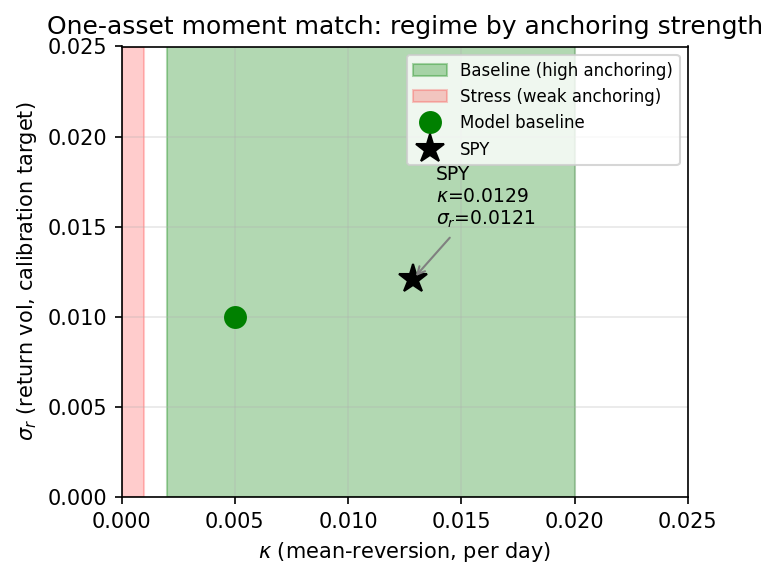
\includegraphics[width=0.48\textwidth]{../paper_artifacts/moment_match/fig_moment_match_regime.png}
  \caption{One-asset moment match: estimated $\kappa$ for SPY vs.\ baseline and stress regions (regime by anchoring strength). $\sigma_r$ shown as calibration target.}
  \label{fig:moment_match_regime}
\end{figure}


\subsection{Parameter regimes and stress diagnostics}
\label{sec:meaningful_regions}

\paragraph{Preview of findings.}
Two distinct notions matter in this model:
(i) \emph{level amplification}---large mispricing/volatility levels under weak anchoring and/or high noise trading; and
(ii) \emph{overconfidence (treatment) effects}---differences in outcomes when increasing perceived signal precision from $k=1$ to $k=3$.
Our simulations show substantial \emph{level amplification} under stress regimes (Table~\ref{tab:mispricing_stress}), while the incremental
$k$-effects on average mispricing are modest in both baseline and stress calibrations (Tables~\ref{tab:metrics}--\ref{tab:mispricing_persistence}).

\subsubsection{Stress regimes: when mispricing \emph{levels} become economically large}
\label{subsec:stress}
Table~\ref{tab:mispricing_stress} reports ``stress diagnostics'' in which anchoring is weakened ($\kappa$ reduced) and/or noise trading increases ($\phi$ increased).
Weak anchoring and high $\phi$ generate large mispricing and volatility \emph{levels} (e.g., $\E[|p-v|]$ exceeding $3$--$9$ in stress cases vs.\ $\approx 1.9$ in baseline).
\textbf{Importantly, these level shifts are primarily driven by $(\kappa,\phi)$: within each stress case, outcomes are nearly unchanged between $k=1$ and $k=3$.}
This demonstrates that level amplification comes from market microstructure parameters (anchoring strength, noise trading) rather than the overconfidence treatment.

\subsubsection{Baseline benchmark: \texorpdfstring{$k$}{k} primarily increases disagreement and trading intensity}
\label{subsec:baseline_benchmark}
We next report the baseline bull/bear scenarios under the benchmark calibration (Table~\ref{tab:params}).
In this parameterization, increasing overconfidence primarily increases cross-sectional disagreement and trading intensity
(e.g., $\Delta \E[\sigma_i(\hat v_i)] \approx +0.059$ and $\Delta \E[\sigma_i(x_i)] \approx +0.001$), while changes in mean absolute mispricing remain modest ($|\Delta \E[|p-v|]| \approx 0.004$).
Mispricing tail and persistence diagnostics (Table~\ref{tab:mispricing_persistence}) are essentially unchanged across $k$.
This baseline serves as a robustness check: it demonstrates that the model does not always amplify mispricing, and that overconfidence's primary channel is through belief dispersion and trading intensity rather than price levels.

\subsubsection{Targeted joint-move grid: \texorpdfstring{$k$}{k}-effects on mispricing are robustly small}
\label{subsec:joint_grid}
A natural concern is that one-at-a-time sweeps may miss interaction effects: overconfidence-induced amplification might require
\emph{simultaneous} changes in anchoring strength, price impact, and noise trading. To test this directly, we run a targeted
$3\times 3\times 3$ grid over $(\kappa,\lambda,\phi)$ in the bull regime using paired random seeds and compare
$k=3$ against $k=1$ within each cell.

Table~\ref{tab:joint_grid} reports cell-by-cell differences in key diagnostics, and
Figures~\ref{fig:joint_grid_mispricing}--\ref{fig:joint_grid_disagreement} visualize the resulting treatment effects.
We classify a cell as \emph{non-negligible} if (i) the 95\% confidence interval for $\Delta_k \E[|p-v|]$ excludes zero and
(ii) $|\Delta_k \E[|p-v|]|$ exceeds 5\% of the baseline $\E[|p-v|]$ in the same cell.

\textbf{Negative result (robust across the joint grid).}
Across the full joint grid, $k=3-1$ differences in $\E[|p-v|]$ are economically small: in Table~\ref{tab:joint_grid}, $\Delta_k\E[|p-v|]$ ranges from $0$ to about $-0.02$ and only $2$ out of $27$ cells meet our ``non-negligible'' flag threshold.
In several cells the 95\% confidence interval excludes zero, but the magnitude remains small relative to the baseline mispricing level (order $1$--$10$ depending on the regime),
including in cells where weak anchoring and high noise trading generate large \emph{levels} of mispricing.
By contrast, disagreement and trading-intensity proxies move systematically with $k$.
In this architecture, overconfidence primarily loads onto belief dispersion and trading intensity rather than price-level mispricing.
% Optional robustness: (i) Bear-regime repeat of the same grid; (ii) Report largest $|\Delta_k \E[|p-v|]|$ cell even if below 5\% threshold.

\begin{table}[t]
  \centering
  \scriptsize
  \setlength{\tabcolsep}{3pt}
  \resizebox{\columnwidth}{!}{\begin{tabular}{rrrcccccc}
\hline
$\phi$ & $\kappa$ & $\lambda$ & $\Delta\E[|p-v|]$ & $\Delta\E[\sigma_i(\hat v_i)]$ & $\Delta\E[|x_i|]$ & $\Delta\,\mathrm{std}(\sum_i x_i)$ & $\Delta\,\mathrm{std}(r)$ & Flag \\
\hline
0.25 & 0.001 & 0.10 & $-0.000\pm0.004$ & $0.059\pm0.000$ & $0.000\pm0.000$ & $0.038\pm0.055$ & $-0.000\pm0.000$ &  \\
0.25 & 0.001 & 0.20 & $-0.004\pm0.005$ & $0.059\pm0.000$ & $0.000\pm0.000$ & $0.049\pm0.084$ & $-0.000\pm0.000$ &  \\
0.25 & 0.001 & 0.50 & $-0.013\pm0.004$ & $0.059\pm0.000$ & $0.001\pm0.001$ & $0.150\pm0.125$ & $0.000\pm0.000$ &  \\
0.25 & 0.005 & 0.10 & $-0.006\pm0.005$ & $0.059\pm0.000$ & $0.001\pm0.001$ & $0.230\pm0.247$ & $-0.000\pm0.000$ &  \\
0.25 & 0.005 & 0.20 & $-0.012\pm0.004$ & $0.059\pm0.000$ & $0.002\pm0.001$ & $0.394\pm0.297$ & $0.000\pm0.000$ &  \\
0.25 & 0.005 & 0.50 & $-0.019\pm0.003$ & $0.059\pm0.000$ & $0.002\pm0.001$ & $0.507\pm0.173$ & $0.001\pm0.000$ & $\checkmark$ \\
0.25 & 0.020 & 0.10 & $-0.012\pm0.003$ & $0.059\pm0.000$ & $0.007\pm0.003$ & $1.209\pm0.650$ & $0.000\pm0.000$ &  \\
0.25 & 0.020 & 0.20 & $-0.017\pm0.003$ & $0.059\pm0.000$ & $0.007\pm0.002$ & $1.197\pm0.435$ & $0.000\pm0.000$ &  \\
0.25 & 0.020 & 0.50 & $-0.019\pm0.003$ & $0.059\pm0.000$ & $0.004\pm0.002$ & $0.739\pm0.373$ & $0.001\pm0.001$ & $\checkmark$ \\
0.50 & 0.001 & 0.10 & $-0.000\pm0.001$ & $0.059\pm0.000$ & $0.000\pm0.000$ & $0.005\pm0.009$ & $-0.000\pm0.000$ &  \\
0.50 & 0.001 & 0.20 & $-0.001\pm0.003$ & $0.059\pm0.000$ & $0.000\pm0.000$ & $0.006\pm0.027$ & $-0.000\pm0.000$ &  \\
0.50 & 0.001 & 0.50 & $-0.002\pm0.004$ & $0.059\pm0.000$ & $0.000\pm0.000$ & $0.002\pm0.016$ & $-0.000\pm0.000$ &  \\
0.50 & 0.005 & 0.10 & $-0.001\pm0.002$ & $0.059\pm0.000$ & $0.000\pm0.000$ & $0.016\pm0.051$ & $-0.000\pm0.000$ &  \\
0.50 & 0.005 & 0.20 & $-0.005\pm0.005$ & $0.059\pm0.000$ & $0.000\pm0.001$ & $0.042\pm0.116$ & $-0.000\pm0.000$ &  \\
0.50 & 0.005 & 0.50 & $-0.007\pm0.005$ & $0.059\pm0.000$ & $0.000\pm0.000$ & $0.027\pm0.064$ & $-0.000\pm0.000$ &  \\
0.50 & 0.020 & 0.10 & $-0.003\pm0.002$ & $0.059\pm0.000$ & $0.001\pm0.001$ & $0.132\pm0.181$ & $-0.000\pm0.000$ &  \\
0.50 & 0.020 & 0.20 & $-0.008\pm0.004$ & $0.059\pm0.000$ & $0.001\pm0.001$ & $0.295\pm0.320$ & $0.000\pm0.000$ &  \\
0.50 & 0.020 & 0.50 & $-0.009\pm0.004$ & $0.059\pm0.000$ & $0.001\pm0.001$ & $0.152\pm0.154$ & $0.000\pm0.000$ &  \\
1.50 & 0.001 & 0.10 & $-0.000\pm0.000$ & $0.059\pm0.000$ & $0.000\pm0.000$ & $0.000\pm0.001$ & $-0.000\pm0.000$ &  \\
1.50 & 0.001 & 0.20 & $-0.000\pm0.000$ & $0.059\pm0.000$ & $0.000\pm0.000$ & $0.000\pm0.001$ & $-0.000\pm0.000$ &  \\
1.50 & 0.001 & 0.50 & $-0.000\pm0.000$ & $0.059\pm0.000$ & $0.000\pm0.000$ & $0.000\pm0.001$ & $-0.000\pm0.000$ &  \\
1.50 & 0.005 & 0.10 & $-0.000\pm0.000$ & $0.059\pm0.000$ & $0.000\pm0.000$ & $0.000\pm0.004$ & $-0.000\pm0.000$ &  \\
1.50 & 0.005 & 0.20 & $-0.000\pm0.000$ & $0.059\pm0.000$ & $0.000\pm0.000$ & $0.000\pm0.004$ & $-0.000\pm0.000$ &  \\
1.50 & 0.005 & 0.50 & $-0.001\pm0.001$ & $0.059\pm0.000$ & $0.000\pm0.000$ & $-0.000\pm0.004$ & $-0.000\pm0.000$ &  \\
1.50 & 0.020 & 0.10 & $-0.000\pm0.000$ & $0.059\pm0.000$ & $0.000\pm0.000$ & $0.004\pm0.016$ & $-0.000\pm0.000$ &  \\
1.50 & 0.020 & 0.20 & $-0.001\pm0.001$ & $0.059\pm0.000$ & $0.000\pm0.000$ & $0.004\pm0.016$ & $-0.000\pm0.000$ &  \\
1.50 & 0.020 & 0.50 & $-0.001\pm0.001$ & $0.059\pm0.000$ & $0.000\pm0.000$ & $0.004\pm0.017$ & $-0.000\pm0.000$ &  \\
\hline
\end{tabular}
}
  \caption{Joint-grid treatment effects $\Delta_k$ across $(\kappa,\lambda,\phi)$ (Bull regime; $\Delta$ denotes $k=3$ minus $k=1$; mean $\pm$ 95\% CI across paired seeds; ``Flag'' per thresholds in text).}
  \label{tab:joint_grid}
\end{table}

\begin{figure}[t]
  \centering
  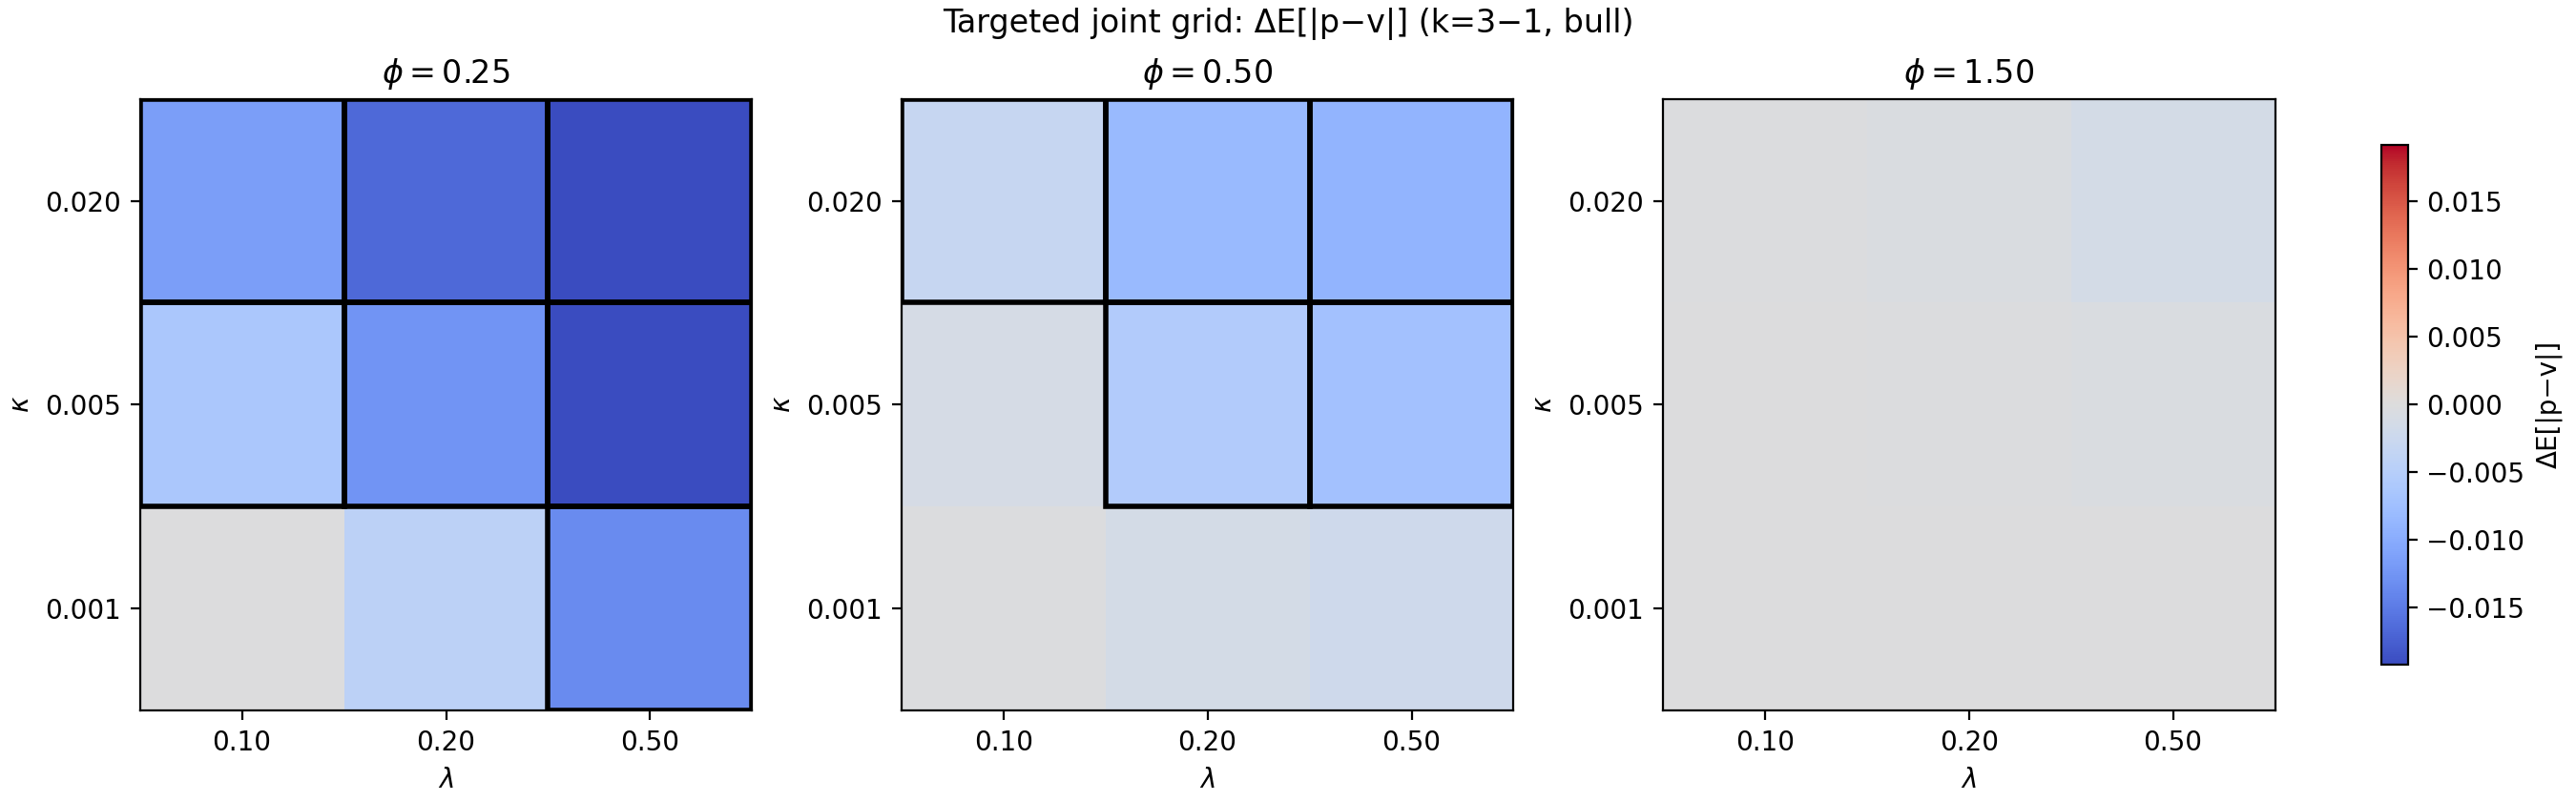
\includegraphics[width=0.95\linewidth]{../paper_artifacts/figures/fig_joint_move_grid_mispricing.png}
  \caption{Joint-grid treatment effects $\Delta_k \E[|p-v|]$ across $(\kappa,\lambda)$ for three $\phi$ slices.}
  \label{fig:joint_grid_mispricing}
\end{figure}

\begin{figure}[t]
  \centering
  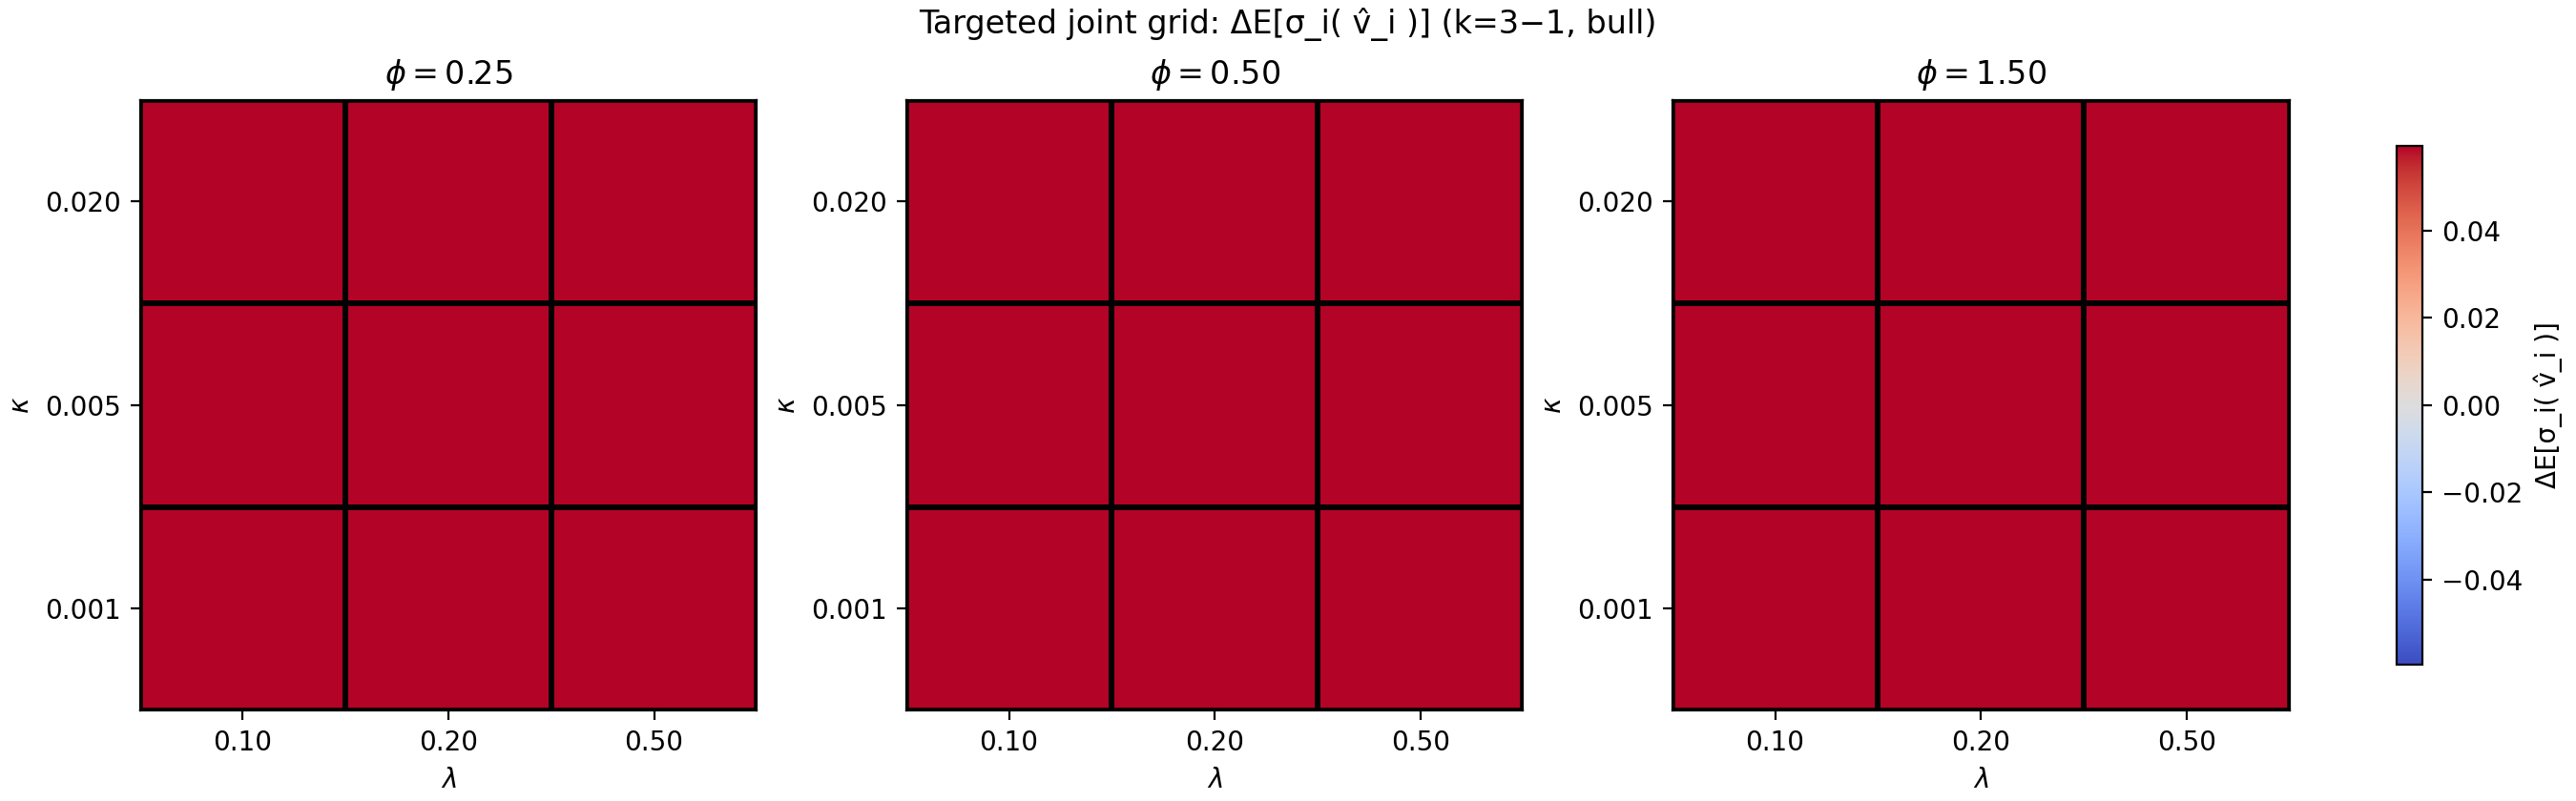
\includegraphics[width=0.95\linewidth]{../paper_artifacts/figures/fig_joint_move_grid_disagreement.png}
  \caption{Joint-grid treatment effects on disagreement $\Delta_k \E[\sigma_i(\hat v_i)]$ across $(\kappa,\lambda)$ for three $\phi$ slices.}
  \label{fig:joint_grid_disagreement}
\end{figure}

\subsubsection{One-at-a-time sweeps: why they rarely generate large \texorpdfstring{$k$}{k}-effects}
\label{subsec:sweeps}
The joint-grid above (Subsection~\ref{subsec:joint_grid}) establishes that we checked the obvious concern: simultaneous changes in $(\kappa,\lambda,\phi)$ do not reveal hidden $k$-driven mispricing amplification. We now report one-at-a-time sweeps over the key levers highlighted by the model: the impact-to-anchoring ratio $(\lambda/\kappa)$,
signal-to-noise in private information, anchoring strength $\kappa$, and regime drift magnitude $|\mu_v|$.

\textbf{Economic significance (Flag).}
The ``Flag'' column in Tables~\ref{tab:lambda_kappa_sweep}--\ref{tab:regime_strength_sweep} and in the joint grid (Table~\ref{tab:joint_grid}) marks cells where the $k=3{-}1$ effect is \emph{economically meaningful} by the following criteria.
\emph{Mispricing:} we flag if $|\Delta\E[|p-v|]| \ge \max(\theta_{\mathrm{abs}},\ \theta_{\mathrm{rel}}\times \text{baseline }\E[|p-v|])$.
For the one-at-a-time sweeps we use $\theta_{\mathrm{rel}}=10\%$ and $\theta_{\mathrm{abs}}=0.10$; for the joint grid we use $\theta_{\mathrm{rel}}=5\%$ and $\theta_{\mathrm{abs}}=0$ so that any cell with a nontrivial relative change in mispricing is flagged; the impaired-arbitrage extension (Table~\ref{tab:extension_state_dependent}) uses $\theta_{\mathrm{rel}}=5\%$ and $\theta_{\mathrm{abs}}=0.05$.
\emph{Return volatility:} we flag if $|\Delta\,\mathrm{std}(r)| \ge 20\%$ of the baseline $\mathrm{std}(r)$ in that cell.
These thresholds are chosen so that ``meaningful'' corresponds to a material relative change in mispricing (5--10\% of baseline) or a substantive change in return volatility (20\%); in our baseline, $\E[|p-v|]\approx 1.9$ (Table~\ref{tab:metrics}), so $\theta_{\mathrm{abs}}=0.10$ is about 5\% of baseline.
A sensitivity check using $\theta_{\mathrm{rel}}\in\{5\%,15\%\}$ for mispricing and 15\% or 25\% for return volatility leaves the set of flagged cells nearly unchanged in our sweeps; the conclusion that $k$-effects on mispricing are small is robust to these alternatives.

\textbf{Across one-at-a-time sweeps (Tables~\ref{tab:lambda_kappa_sweep}--\ref{tab:regime_strength_sweep}), $k$-effects on mispricing diagnostics remain small, consistent with the baseline's strong anchoring channel ($\kappa=0.005$) suppressing mispricing regardless of other parameters.}
Even when sweeping impact strength $\lambda$ up to $0.50$ (Table~\ref{tab:lambda_kappa_sweep}), the $k$-effect on mispricing remains small (often negative) because anchoring remains strong.
The sweeps therefore map where outcomes become fragile in \emph{levels} and clarify which parameters would need to be jointly re-estimated in a full calibration exercise targeting economically meaningful mispricing episodes.

\begin{table}[t]
  \centering
  \scriptsize
  \setlength{\tabcolsep}{3pt}
  \resizebox{\columnwidth}{!}{\begin{tabular}{rrcccccc}
\hline
$\lambda$ (impact) & $\lambda/\kappa$ & $\Delta\E[|p-v|]$ & $\Delta q_{0.95}(|p-v|)$ & $\Delta q_{0.99}(|p-v|)$ & $\Delta\,\mathrm{std}(r)$ & $\Delta\,\rho_1(|r|)$ & Flag \\
\hline
0.10 & 20.0 & $0.000\pm0.002$ & $-0.002\pm0.005$ & $-0.004\pm0.003$ & $-0.000\pm0.000$ & $-0.000\pm0.000$ &  \\
0.20 & 40.0 & $-0.000\pm0.005$ & $-0.012\pm0.012$ & $-0.009\pm0.015$ & $-0.000\pm0.000$ & $-0.000\pm0.000$ &  \\
0.30 & 60.0 & $0.000\pm0.005$ & $-0.002\pm0.012$ & $-0.008\pm0.010$ & $-0.000\pm0.000$ & $-0.000\pm0.000$ &  \\
0.40 & 80.0 & $-0.001\pm0.005$ & $-0.010\pm0.014$ & $-0.013\pm0.013$ & $-0.000\pm0.000$ & $-0.000\pm0.000$ &  \\
0.50 & 100.0 & $-0.001\pm0.006$ & $-0.009\pm0.012$ & $-0.013\pm0.018$ & $-0.000\pm0.000$ & $-0.000\pm0.000$ &  \\
0.75 & 150.0 & $-0.004\pm0.006$ & $-0.023\pm0.018$ & $-0.032\pm0.018$ & $-0.000\pm0.000$ & $0.000\pm0.001$ &  \\
1.00 & 200.0 & $-0.006\pm0.005$ & $-0.040\pm0.024$ & $-0.029\pm0.022$ & $0.000\pm0.000$ & $0.000\pm0.001$ &  \\
\hline
\end{tabular}
}
  \caption{Impact-to-anchoring sweep (Bull regime). $\Delta$ denotes $k=3$ minus $k=1$; ``Flag'' marks economically meaningful regions (see text for thresholds).}
  \label{tab:lambda_kappa_sweep}
\end{table}

\begin{figure}[t]
  \centering
  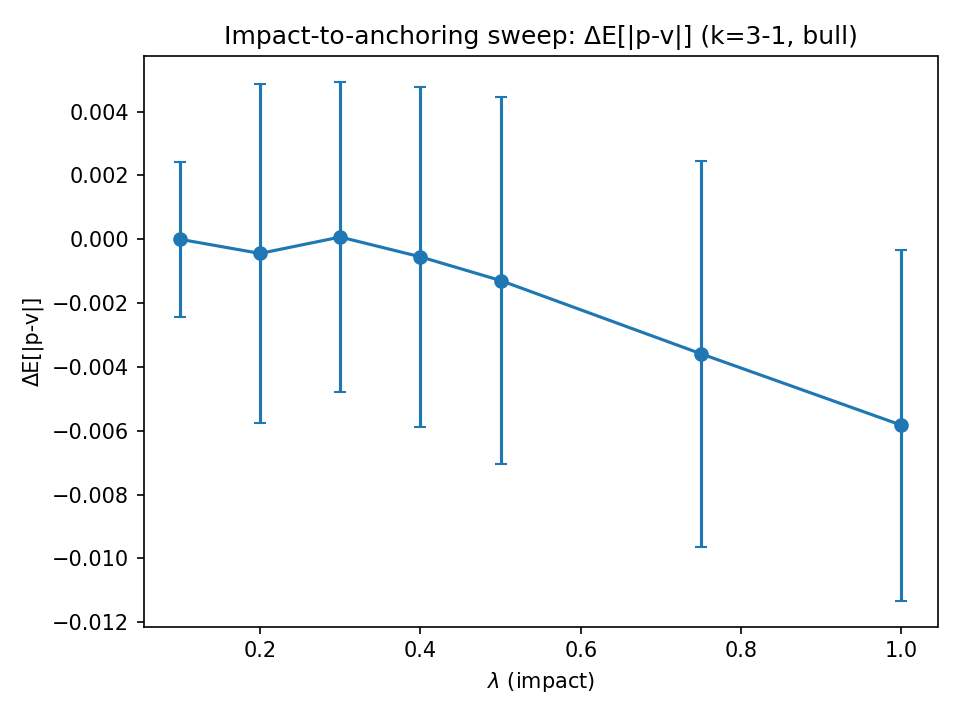
\includegraphics[width=0.48\textwidth]{../paper_artifacts/figures/fig_lambda_kappa_sweep_mispricing.png}
  \caption{Effect of $\lambda$ (impact) on $\Delta\E[|p-v|]$ (Bull regime; $\Delta$ denotes $k=3$ minus $k=1$).}
  \label{fig:lambda_kappa_sweep_mispricing}
\end{figure}

\begin{figure}[t]
  \centering
  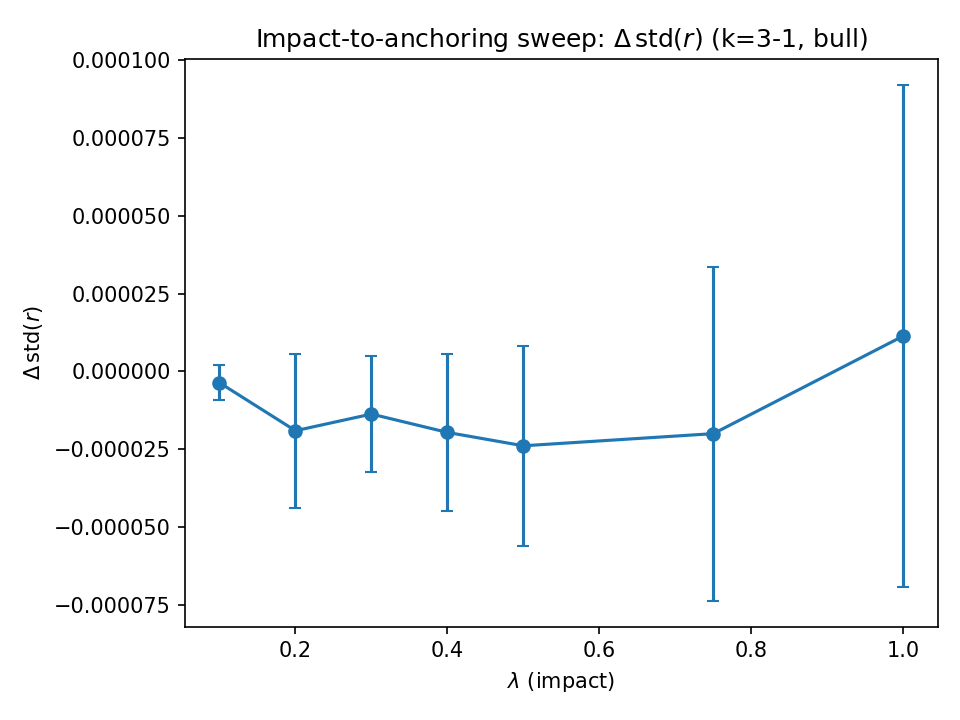
\includegraphics[width=0.48\textwidth]{../paper_artifacts/figures/fig_lambda_kappa_sweep_volatility.png}
  \caption{Effect of $\lambda$ (impact) on $\Delta\,\mathrm{std}(r)$ (Bull regime; $\Delta$ denotes $k=3$ minus $k=1$).}
  \label{fig:lambda_kappa_sweep_volatility}
\end{figure}

\begin{table}[t]
  \centering
  \scriptsize
  \setlength{\tabcolsep}{3pt}
  \resizebox{\columnwidth}{!}{\begin{tabular}{rrcccccccc}
\hline
$\sigma_\epsilon$ & $\sigma_v/\sigma_\epsilon$ & $\Delta\E[|p-v|]$ & $\Delta q_{0.95}(|p-v|)$ & $\Delta q_{0.99}(|p-v|)$ & $\Delta\,\mathrm{std}(r)$ & $\Delta\,\rho_1(|r|)$ & $\Delta\E[\sigma_i(\hat v_i)]$ & $\Delta\E[\sigma_i(x_i)]$ & Flag \\
\hline
0.40 & 0.250 & $-0.002\pm0.003$ & $-0.005\pm0.007$ & $-0.007\pm0.007$ & $-0.000\pm0.000$ & $-0.000\pm0.000$ & $0.037\pm0.000$ & $0.001\pm0.000$ &  \\
0.50 & 0.200 & $-0.003\pm0.003$ & $-0.008\pm0.009$ & $-0.007\pm0.007$ & $-0.000\pm0.000$ & $0.000\pm0.000$ & $0.044\pm0.000$ & $0.001\pm0.000$ &  \\
0.60 & 0.167 & $-0.003\pm0.004$ & $-0.009\pm0.011$ & $-0.007\pm0.009$ & $-0.000\pm0.000$ & $0.000\pm0.000$ & $0.050\pm0.000$ & $0.001\pm0.000$ &  \\
0.80 & 0.125 & $-0.004\pm0.006$ & $-0.009\pm0.013$ & $-0.007\pm0.012$ & $-0.000\pm0.000$ & $0.000\pm0.000$ & $0.060\pm0.000$ & $0.001\pm0.000$ &  \\
1.00 & 0.100 & $-0.005\pm0.007$ & $-0.009\pm0.013$ & $-0.009\pm0.014$ & $-0.000\pm0.000$ & $0.000\pm0.000$ & $0.068\pm0.000$ & $0.001\pm0.000$ &  \\
1.20 & 0.083 & $-0.005\pm0.008$ & $-0.007\pm0.015$ & $-0.010\pm0.016$ & $-0.000\pm0.000$ & $0.000\pm0.000$ & $0.075\pm0.000$ & $0.002\pm0.000$ &  \\
2.00 & 0.050 & $-0.007\pm0.012$ & $-0.021\pm0.022$ & $-0.021\pm0.017$ & $-0.000\pm0.000$ & $0.000\pm0.000$ & $0.100\pm0.000$ & $0.002\pm0.000$ &  \\
\hline
\end{tabular}
}
  \caption{Signal-to-noise sweep (Bull regime): varying $\sigma_\epsilon$ while holding $\sigma_v$ fixed. ``Flag'' marks economically meaningful regions (see text).}
  \label{tab:signal_to_noise_sweep}
\end{table}

\begin{figure}[t]
  \centering
  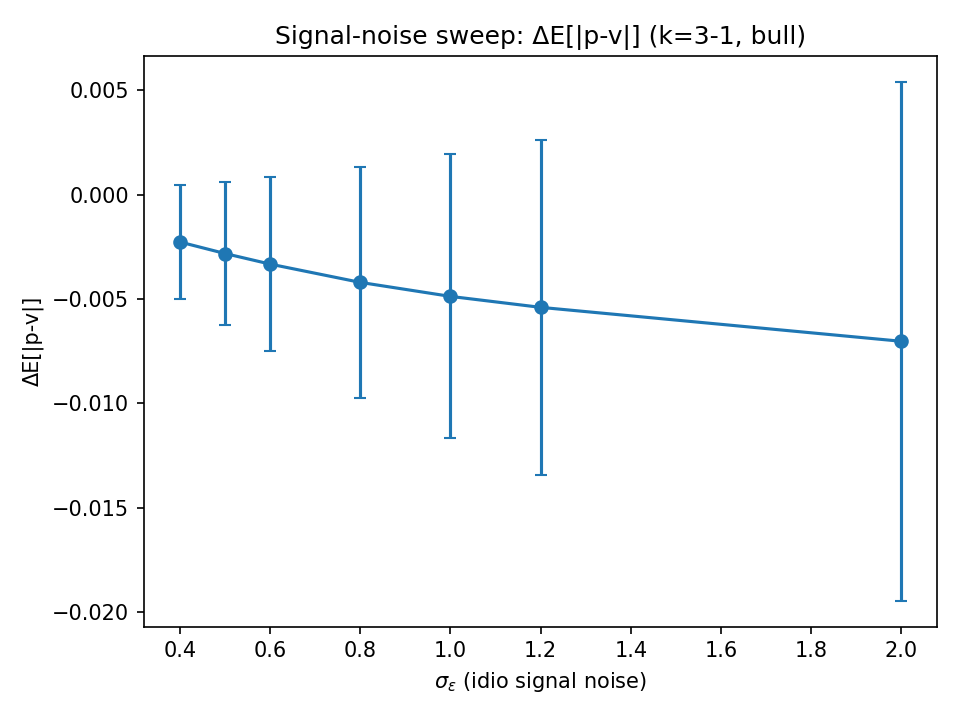
\includegraphics[width=0.48\textwidth]{../paper_artifacts/figures/fig_signal_to_noise_sweep_mispricing.png}
  \caption{Effect of $\sigma_\epsilon$ on $\Delta\E[|p-v|]$ (Bull regime; $\Delta$ denotes $k=3$ minus $k=1$).}
  \label{fig:signal_to_noise_sweep_mispricing}
\end{figure}

\begin{figure}[t]
  \centering
  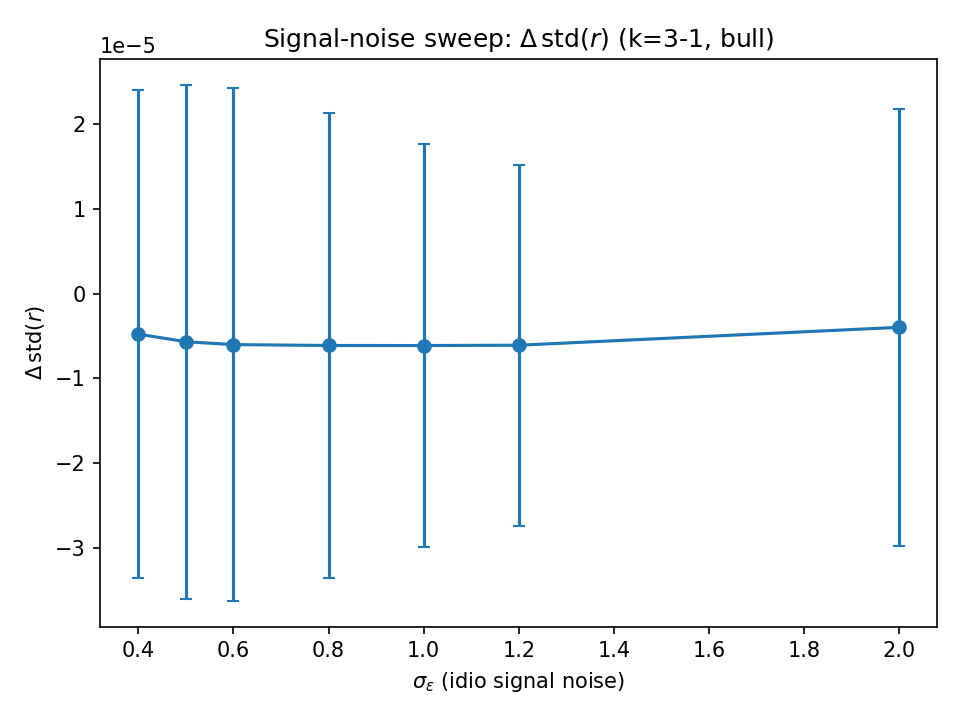
\includegraphics[width=0.48\textwidth]{../paper_artifacts/figures/fig_signal_to_noise_sweep_volatility.png}
  \caption{Effect of $\sigma_\epsilon$ on $\Delta\,\mathrm{std}(r)$ (Bull regime; $\Delta$ denotes $k=3$ minus $k=1$).}
  \label{fig:signal_to_noise_sweep_volatility}
\end{figure}

\begin{table}[t]
  \centering
  \scriptsize
  \setlength{\tabcolsep}{3pt}
  \resizebox{\columnwidth}{!}{\begin{tabular}{rrcccccc}
\hline
$\kappa$ & $\lambda/\kappa$ & $\Delta\E[|p-v|]$ & $\Delta q_{0.95}(|p-v|)$ & $\Delta q_{0.99}(|p-v|)$ & $\Delta\,\mathrm{std}(r)$ & $\Delta\,\rho_1(|r|)$ & Flag \\
\hline
0.001 & 200.0 & $0.001\pm0.003$ & $-0.003\pm0.005$ & $-0.002\pm0.006$ & $0.000\pm0.000$ & $0.000\pm0.000$ &  \\
0.002 & 100.0 & $0.000\pm0.004$ & $-0.000\pm0.007$ & $-0.004\pm0.007$ & $0.000\pm0.000$ & $0.000\pm0.000$ &  \\
0.003 & 66.7 & $-0.000\pm0.005$ & $-0.009\pm0.005$ & $-0.009\pm0.010$ & $0.000\pm0.000$ & $0.000\pm0.000$ &  \\
0.005 & 40.0 & $-0.002\pm0.004$ & $-0.010\pm0.011$ & $-0.015\pm0.010$ & $0.000\pm0.000$ & $0.000\pm0.000$ &  \\
0.010 & 20.0 & $-0.004\pm0.003$ & $-0.007\pm0.013$ & $-0.010\pm0.024$ & $0.000\pm0.000$ & $0.000\pm0.000$ &  \\
0.020 & 10.0 & $-0.004\pm0.003$ & $-0.011\pm0.014$ & $-0.017\pm0.025$ & $0.000\pm0.000$ & $-0.000\pm0.000$ &  \\
\hline
\end{tabular}
}
  \caption{Anchoring sweep (Bull regime): varying $\kappa$ at fixed $(\lambda,\phi)$. ``Flag'' marks economically meaningful regions (see text).}
  \label{tab:kappa_sweep}
\end{table}

\begin{table}[t]
  \centering
  \scriptsize
  \setlength{\tabcolsep}{3pt}
  \resizebox{\columnwidth}{!}{\begin{tabular}{lrcccccc}
\hline
Regime & $\mu_v$ & $\Delta\E[|p-v|]$ & $\Delta q_{0.95}(|p-v|)$ & $\Delta q_{0.99}(|p-v|)$ & $\Delta\,\mathrm{std}(r)$ & $\Delta\,\rho_1(|r|)$ & Flag \\
\hline
Bull & 0.010 & $-0.009\pm0.004$ & $-0.012\pm0.018$ & $-0.024\pm0.018$ & $-0.000\pm0.000$ & $-0.000\pm0.000$ &  \\
Bull & 0.020 & $-0.009\pm0.005$ & $-0.011\pm0.015$ & $-0.020\pm0.021$ & $-0.000\pm0.000$ & $-0.000\pm0.000$ &  \\
Bull & 0.030 & $-0.009\pm0.005$ & $-0.016\pm0.019$ & $-0.020\pm0.021$ & $-0.000\pm0.000$ & $-0.000\pm0.000$ &  \\
Bull & 0.050 & $-0.008\pm0.007$ & $-0.011\pm0.015$ & $-0.013\pm0.021$ & $-0.000\pm0.000$ & $-0.000\pm0.000$ &  \\
Bear & -0.010 & $-0.009\pm0.004$ & $-0.028\pm0.015$ & $-0.031\pm0.017$ & $-0.000\pm0.000$ & $-0.000\pm0.000$ &  \\
Bear & -0.020 & $-0.009\pm0.004$ & $-0.023\pm0.014$ & $-0.021\pm0.019$ & $-0.000\pm0.000$ & $-0.000\pm0.000$ &  \\
Bear & -0.030 & $-0.008\pm0.005$ & $-0.019\pm0.021$ & $-0.018\pm0.020$ & $-0.000\pm0.000$ & $-0.000\pm0.000$ &  \\
Bear & -0.050 & $-0.007\pm0.007$ & $-0.009\pm0.025$ & $-0.018\pm0.025$ & $-0.000\pm0.000$ & $-0.000\pm0.000$ &  \\
\hline
\end{tabular}
}
  \caption{Regime-strength sweep: varying $|\mu_v|$ in bull/bear regimes. ``Flag'' marks economically meaningful regions (see text).}
  \label{tab:regime_strength_sweep}
\end{table}

\begin{table}[t]
  \centering
  \scriptsize
  \setlength{\tabcolsep}{3pt}
  \resizebox{\columnwidth}{!}{\begin{tabular}{lrrcccccc}
\hline
Scenario & $\kappa$ & $\phi$ & \multicolumn{2}{c}{$\E[|p-v|]$} & \multicolumn{2}{c}{$q_{0.95}(|p-v|)$} & \multicolumn{2}{c}{$\mathrm{std}(r)$} \\
 &  &  & $k=1$ & $k=3$ & $k=1$ & $k=3$ & $k=1$ & $k=3$ \\
\hline
Baseline & 0.005 & 0.50 & $1.774\pm0.273$ & $1.767\pm0.276$ & $4.164\pm0.634$ & $4.155\pm0.633$ & $0.491\pm0.008$ & $0.491\pm0.008$ \\
Weak anchoring & 0.001 & 0.50 & $3.972\pm1.318$ & $3.969\pm1.320$ & $8.118\pm2.108$ & $8.113\pm2.112$ & $0.488\pm0.008$ & $0.488\pm0.008$ \\
High noise & 0.005 & 1.00 & $6.113\pm1.909$ & $6.112\pm1.910$ & $13.461\pm3.392$ & $13.460\pm3.393$ & $0.977\pm0.015$ & $0.977\pm0.015$ \\
Weak+high & 0.001 & 1.00 & $9.258\pm3.875$ & $9.258\pm3.875$ & $18.993\pm5.852$ & $18.993\pm5.851$ & $0.976\pm0.015$ & $0.976\pm0.015$ \\
Low noise & 0.005 & 0.25 & $0.614\pm0.049$ & $0.599\pm0.049$ & $1.514\pm0.145$ & $1.483\pm0.142$ & $0.249\pm0.004$ & $0.250\pm0.004$ \\
Mid-high noise & 0.005 & 0.75 & $4.377\pm1.290$ & $4.376\pm1.291$ & $9.706\pm2.366$ & $9.704\pm2.367$ & $0.733\pm0.012$ & $0.733\pm0.012$ \\
Very high noise & 0.005 & 1.50 & $9.308\pm2.886$ & $9.307\pm2.886$ & $20.516\pm5.137$ & $20.516\pm5.137$ & $1.465\pm0.023$ & $1.465\pm0.023$ \\
Extreme noise & 0.005 & 2.00 & $12.452\pm3.763$ & $12.452\pm3.763$ & $27.326\pm6.779$ & $27.326\pm6.779$ & $1.954\pm0.031$ & $1.954\pm0.031$ \\
Very weak anchoring & 0.001 & 0.50 & $4.999\pm1.827$ & $4.997\pm1.828$ & $9.910\pm2.868$ & $9.907\pm2.870$ & $0.488\pm0.008$ & $0.488\pm0.008$ \\
\hline
\end{tabular}
}
  \caption{Stress diagnostics: weakening anchoring ($\kappa$) and/or increasing noise trading ($\phi$) can generate large
mispricing and volatility \emph{levels}. Within each stress case, outcomes are nearly unchanged between $k=1$ and $k=3$,
indicating that level amplification is primarily driven by $(\kappa,\phi)$ rather than the overconfidence treatment.}
  \label{tab:mispricing_stress}
\end{table}

\begin{table}[t]
  \centering
  \scriptsize
  \setlength{\tabcolsep}{3pt}
  \resizebox{\columnwidth}{!}{\begin{tabular}{lccccc}
\hline
Case & $\E[|p-v|]$ & $q_{0.95}(|p-v|)$ & $q_{0.99}(|p-v|)$ & $\mathrm{std}(r)$ & $\mathrm{std}_{\mathrm{xs}}(k_i)$ \\
\hline
Fixed k=2.0 & $1.910\pm0.234$ & $4.475\pm0.546$ & $5.380\pm0.685$ & $0.504\pm0.011$ & $0.000\pm0.000$ \\
Uniform[1,3] (mean 2) & $1.658\pm0.183$ & $4.027\pm0.416$ & $5.007\pm0.549$ & $0.499\pm0.012$ & $0.563\pm0.009$ \\
Normal(2,0.5) clipped[1,3] & $1.658\pm0.183$ & $4.027\pm0.417$ & $5.007\pm0.549$ & $0.499\pm0.012$ & $0.469\pm0.015$ \\
\hline
\end{tabular}
}
  \caption{Heterogeneous $k$ at fixed mean $\E[k]=2$: comparing dispersion in confidence under the same market regime. Column $\mathrm{std}_{\mathrm{xs}}(k_i)$ is the cross-sectional standard deviation of $k_i$ across agents, time-averaged.}
  \label{tab:heterogeneous_k}
\end{table}

\subsection{Extensions and Validation Checks}
\label{subsec:extensions}

\subsubsection{Myopic vs.\ intertemporal policy}
The core qualitative decomposition is robust across equilibrium concepts: the main $k$-loading remains on disagreement and trading intensity; price-level mispricing is comparatively less sensitive to $k$ under both myopic and intertemporal LQG policies.
Comparisons use the same random seeds (paired shocks) and regime parameters; only the policy toggle and $k$ differ.
Table~\ref{tab:myopic_intertemporal} and Figures~\ref{fig:myopic_intertemporal_mispricing}--\ref{fig:myopic_intertemporal_decomposition} report the results.
The policy decomposition (Figure~\ref{fig:myopic_intertemporal_decomposition}) confirms the intertemporal hedging term is numerically active.
Mispricing is slightly lower under the intertemporal policy than under the myopic rule, and the $k$-treatment effect remains tiny under both; the modest negative $\Delta\E[|p-v|]$ when increasing $k$ is consistent with stronger perceived precision inducing faster corrective trading against mispricing under strong anchoring, so price levels do not blow out---what changes with $k$ is dispersion and trading intensity rather than the level of mispricing.

\begin{table}[t]
  \centering
  \scriptsize
  \setlength{\tabcolsep}{3pt}
  \resizebox{\columnwidth}{!}{\begin{tabular}{lcccc}
\hline
Policy & $k$ & $\mathbb{E}[|p-v|]$ & $q_{0.95}(|p-v|)$ & $\mathrm{std}(r)$ \\
\hline
Myopic & $1$ & $1.633\pm0.246$ & $3.622\pm0.583$ & $0.493\pm0.015$ \\
Myopic & $3$ & $1.632\pm0.246$ & $3.624\pm0.579$ & $0.493\pm0.016$ \\
Intertemporal & $1$ & $1.284\pm0.132$ & $2.868\pm0.313$ & $0.496\pm0.016$ \\
Intertemporal & $3$ & $1.290\pm0.134$ & $2.878\pm0.311$ & $0.496\pm0.016$ \\
$\Delta$ Myopic ($k=3-1$) & --- & $-0.001\pm0.002$ & $0.002\pm0.011$ & $0.000\pm0.000$ \\
$\Delta$ Intertemporal ($k=3-1$) & --- & $0.006\pm0.004$ & $0.010\pm0.012$ & $-0.000\pm0.000$ \\
\hline
\end{tabular}
}
  \caption{Myopic vs.\ intertemporal policy: $\E[|p-v|]$, $q_{0.95}(|p-v|)$, and $\mathrm{std}(r)$ by policy and $k$.}
  \label{tab:myopic_intertemporal}
\end{table}

\begin{figure}[t]
  \centering
  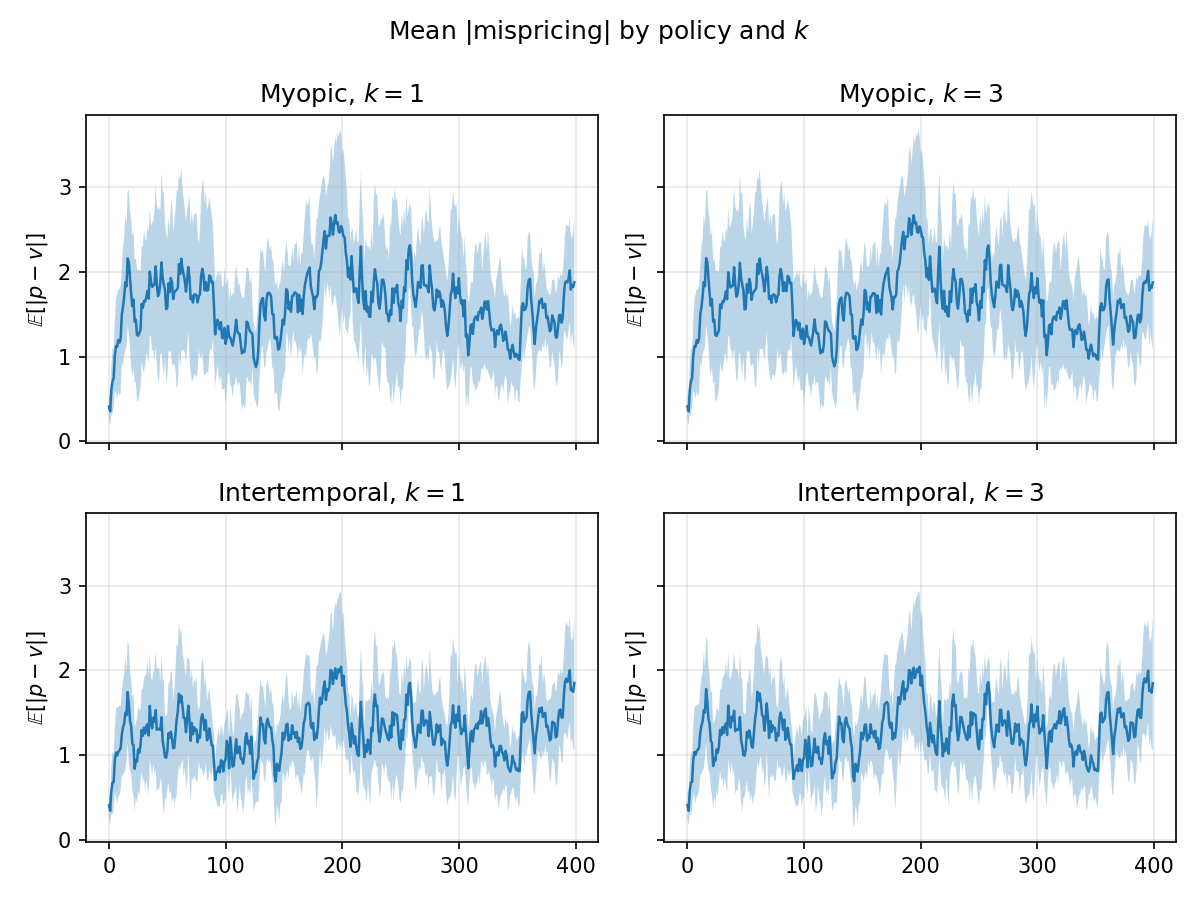
\includegraphics[width=0.95\linewidth]{../paper_artifacts/figures/fig_myopic_intertemporal_mispricing.png}
  \caption{Mean $|p-v|$ by policy (myopic/intertemporal) and $k$ (2$\times$2 grid; 95\% CI bands).}
  \label{fig:myopic_intertemporal_mispricing}
\end{figure}

\begin{figure}[t]
  \centering
  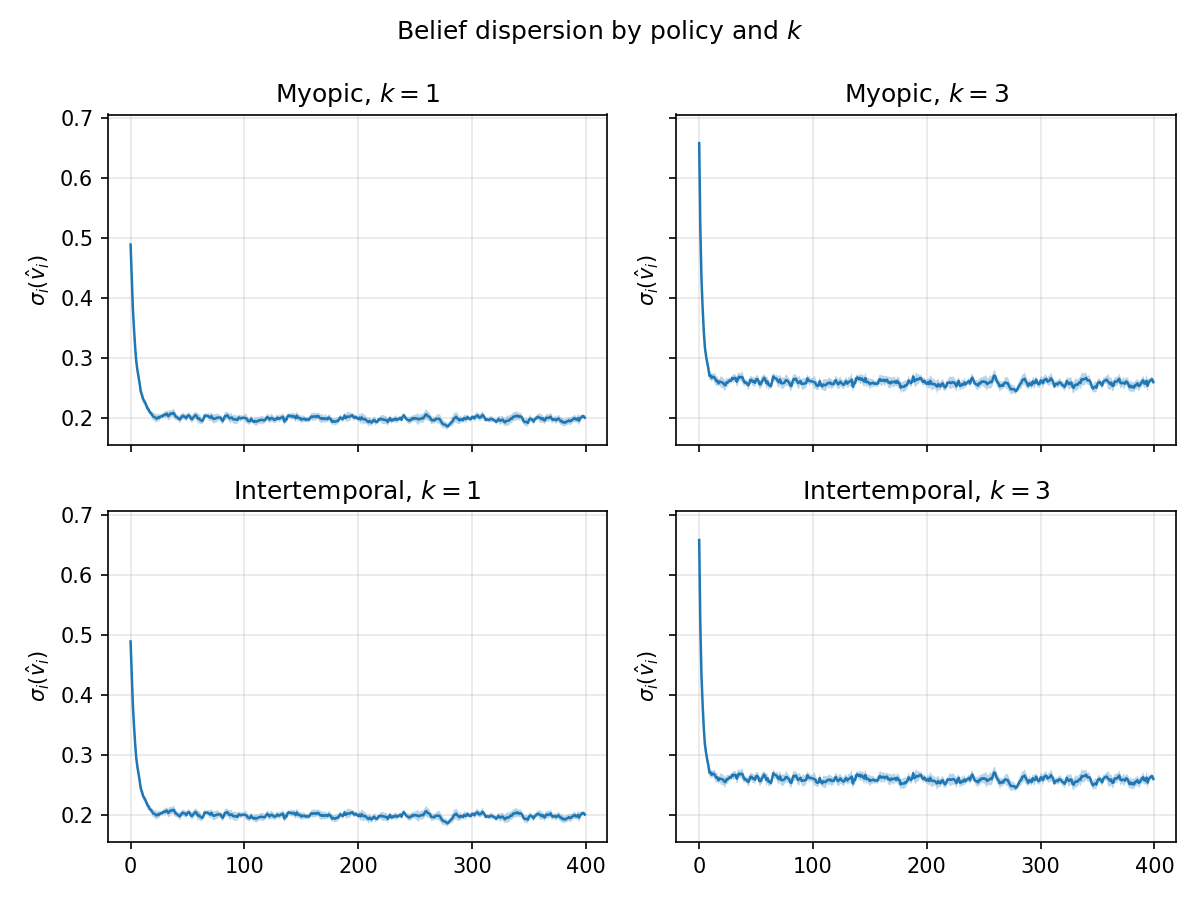
\includegraphics[width=0.95\linewidth]{../paper_artifacts/figures/fig_myopic_intertemporal_disagreement.png}
  \caption{Belief dispersion $\sigma_i(\hat v_i)$ by policy and $k$.}
  \label{fig:myopic_intertemporal_disagreement}
\end{figure}

\begin{figure}[t]
  \centering
  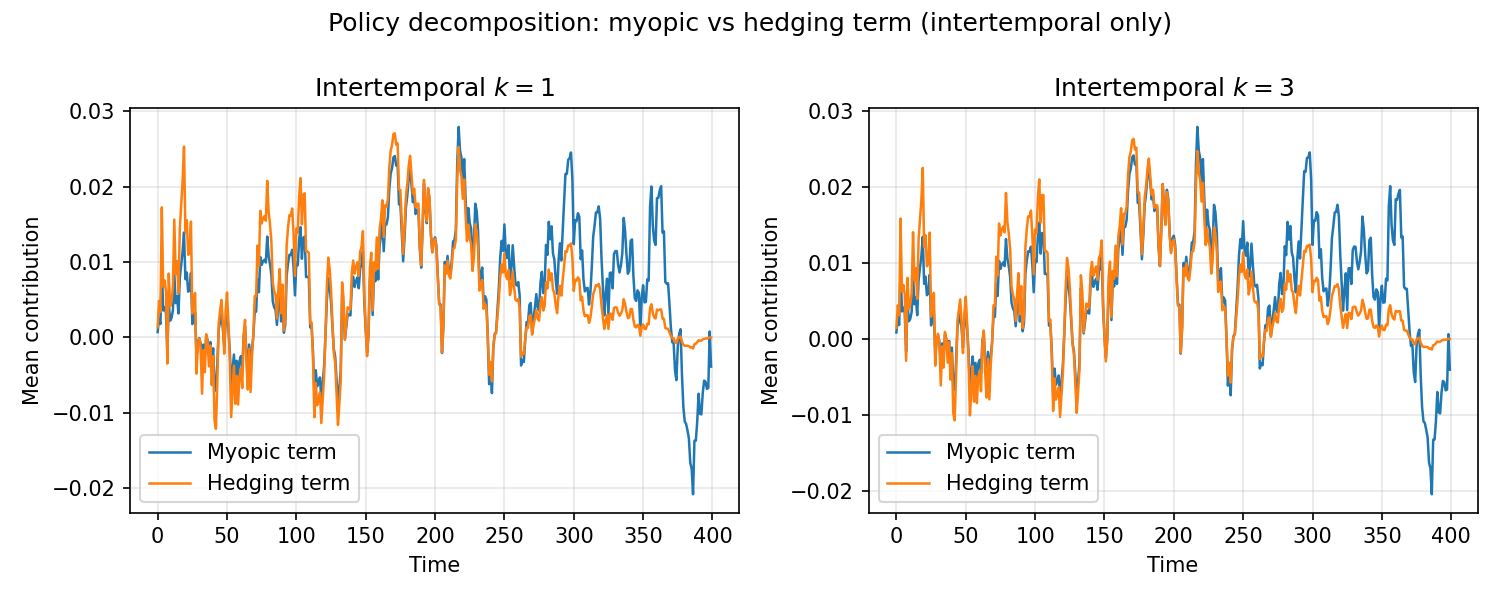
\includegraphics[width=0.95\linewidth]{../paper_artifacts/figures/fig_myopic_intertemporal_policy_decomposition.png}
  \caption{Policy decomposition: myopic vs.\ hedging term contribution (intertemporal runs).}
  \label{fig:myopic_intertemporal_decomposition}
\end{figure}

\subsubsection{Extension: when \texorpdfstring{$k$}{k} can move mispricing}
In the baseline anchored-impact microstructure (relevant for SPY-like regimes), $k$ does not materially move mispricing.
When arbitrage pressure is impaired---e.g., via state-dependent anchoring $\kappa(t)=\kappa_0\exp(-\alpha|p-v|)$ so that $\kappa$ weakens under large mispricing---$k$ can in principle transmit into price-level mispricing.
Table~\ref{tab:extension_state_dependent} and Figure~\ref{fig:extension_state_dependent} report the sensitivity to $\alpha$.
In the parameter range shown ($\alpha\in[0,0.2]$), $\Delta\E[|p-v|]$ ($k=3{-}1$) remains small (around $-0.004$ to $-0.005$); even under modest state-dependence, $k$-effects on mispricing stay small. Larger arbitrage impairment (e.g., higher $\alpha$, lower baseline $\kappa_0$, or higher $\phi$) would be required for $k$ to materially amplify mispricing. The negative result is not built into linearity; it is regime-specific: in the baseline (strong anchoring), $k$ loads onto disagreement/intensity; in sufficiently impaired-arbitrage regimes, $k$ can amplify mispricing.

\begin{table}[t]
  \centering
  \scriptsize
  \setlength{\tabcolsep}{3pt}
  \resizebox{\columnwidth}{!}{\begin{tabular}{rcccccc}
\hline
$\alpha$ & $\E[|p-v|]$ ($k=1$) & $\Delta\E[|p-v|]$ & $\Delta q_{0.5}$ & $\Delta q_{0.95}$ & Flag \\
\hline
0.00 & $1.655$ & $-0.003\pm0.005$ & $-0.000$ & $-0.011$ & $\checkmark$ \\
0.05 & $1.682$ & $-0.003\pm0.005$ & $-0.002$ & $-0.013$ & $\checkmark$ \\
0.10 & $1.707$ & $-0.003\pm0.005$ & $-0.003$ & $-0.010$ & $\checkmark$ \\
0.20 & $1.746$ & $-0.004\pm0.005$ & $0.006$ & $-0.010$ & $\checkmark$ \\
\hline
\end{tabular}
}
  \caption{Impaired-arbitrage extension: $\Delta\E[|p-v|]$ ($k=3{-}1$) vs.\ $\alpha$ (kappa decay rate). ``Flag'' per thresholds in text.}
  \label{tab:extension_state_dependent}
\end{table}

\begin{figure}[t]
  \centering
  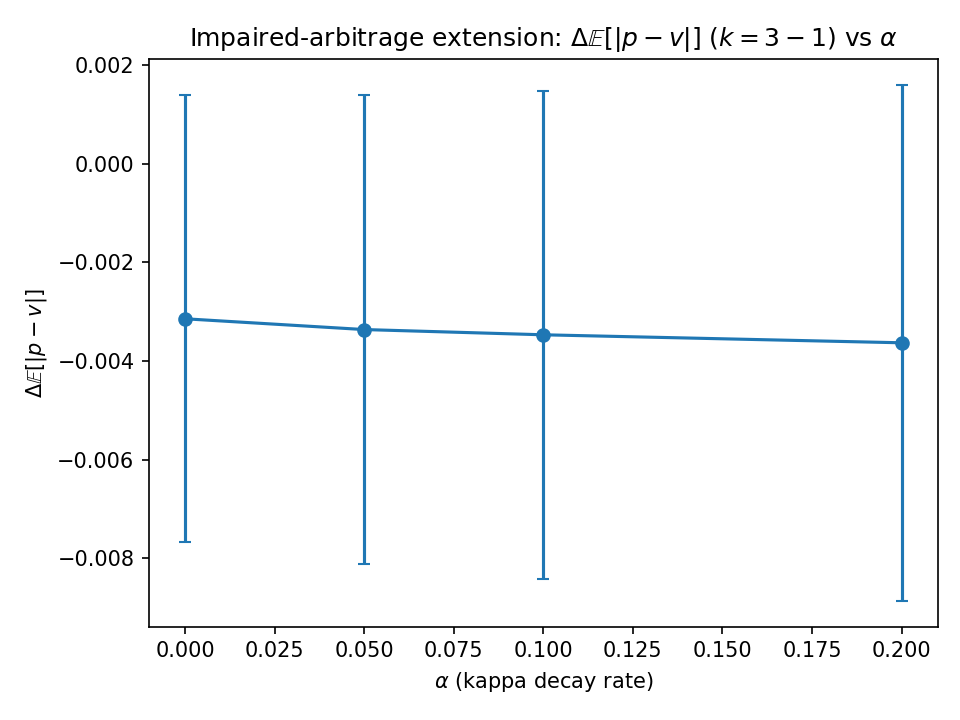
\includegraphics[width=0.48\textwidth]{../paper_artifacts/figures/fig_extension_state_dependent.png}
  \caption{Impaired-arbitrage extension: $\Delta\E[|p-v|]$ ($k=3-1$) vs.\ $\alpha$.}
  \label{fig:extension_state_dependent}
\end{figure}

\subsubsection{Empirical stylized fact: volume and realized return volatility co-movement}
We document a stylized fact consistent with the model's disagreement/intensity channel: volume (log volume) and realized return volatility (rolling standard deviation of daily log returns) co-move positively.
We cannot directly measure belief dispersion without survey/analyst microdata; we use uncertainty proxies as a reduced-form correlate.
This is a well-known generic relationship; we pitch it as external-face validity / sanity check for the model's intensity channel, not as an identification of ``disagreement.'' Analyst forecast dispersion, options-implied disagreement, or survey-based disagreement are natural next steps for tighter empirical tests.
Stress episodes are defined mechanically as the top decile of realized return volatility (no cherry-picking).

\begin{figure}[t]
  \centering
  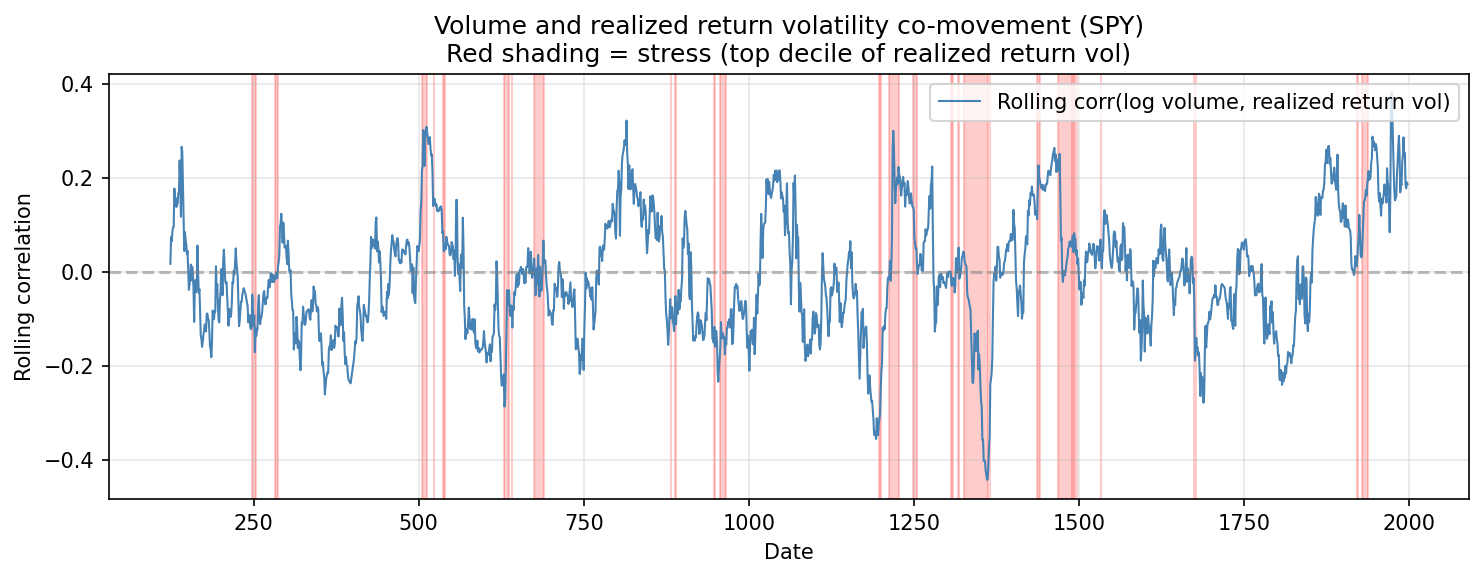
\includegraphics[width=0.95\linewidth]{../paper_artifacts/figures/fig_stylized_volume_volatility.png}
  \caption{Rolling correlation of log volume and realized return volatility (SPY). Red shading = stress (top decile of realized return vol).}
  \label{fig:stylized_volume_volatility}
\end{figure}

\begin{table}[t]
  \centering
  \scriptsize
  \setlength{\tabcolsep}{3pt}
  \resizebox{\columnwidth}{!}{\begin{tabular}{lccc}
\hline
Sample & Correlation & SE & $t$-stat \\
\hline
Full & $-0.018$ & $0.023$ & $-0.766$ \\
Stress (top decile realized vol) & $-0.053$ & $0.073$ & $-0.727$ \\
Non-stress & $-0.025$ & $0.024$ & $-1.009$ \\
\hline
\end{tabular}
}
  \caption{Volume--volatility correlation (log volume vs realized return volatility): full sample, stress, and non-stress (Newey--West $t$-stats).}
  \label{tab:stylized_volume_volatility}
\end{table}

Figure~\ref{fig:stylized_volume_volatility} plots the rolling correlation; Table~\ref{tab:stylized_volume_volatility} reports correlations in stress vs.\ non-stress with Newey--West $t$-statistics.
Our model provides a mechanism: overconfidence increases disagreement and trading intensity; when both are high, volume and belief dispersion move together.

\textbf{Baseline results (benchmark).} Figure~\ref{fig:price_path} reports the mean price path across baseline scenarios. Figure~\ref{fig:mispricing} reports mean absolute mispricing $\E[|p_t-v_t|]$ (computed from the simulated fundamental), and Figure~\ref{fig:volatility} reports a rolling volatility proxy based on realized returns.
Table~\ref{tab:metrics} complements the plots with seed-averaged moments and treatment effects ($k=3$ vs.\ $k=1$). 
\textbf{In this baseline parameterization, the $k$-effect on mispricing is weak ($|\Delta \E[|p-v|]| \approx 0.004$), and mispricing tail/persistence diagnostics (Table~\ref{tab:mispricing_persistence}) are essentially unchanged across $k$.}
Proposition~\ref{prop:mechanism_k} explains this analytically: the mean-field closure depends only on the mean belief $m_t-p_t$, so mispricing is driven by microstructure $(\kappa,\lambda,\phi)$ and the mean-belief error $e_t=m_t-v_t$; under the filter structure, $k$ raises disagreement (strictly in $k$) and trading intensity while affecting the mean belief only weakly, hence small price effects.
Increasing overconfidence primarily increases cross-sectional disagreement and trading intensity (e.g., $\Delta \E[\sigma_i(\hat v_i)] \approx +0.059$ and lower perceived $\E[\bar\Sigma]$), consistent with that mechanism.
The qualitative asymmetry remains visible in paths: bull regimes exhibit more persistent overvaluation episodes, while bear regimes exhibit noisier oscillations around fundamentals.

\begin{figure}[t]
  \centering
  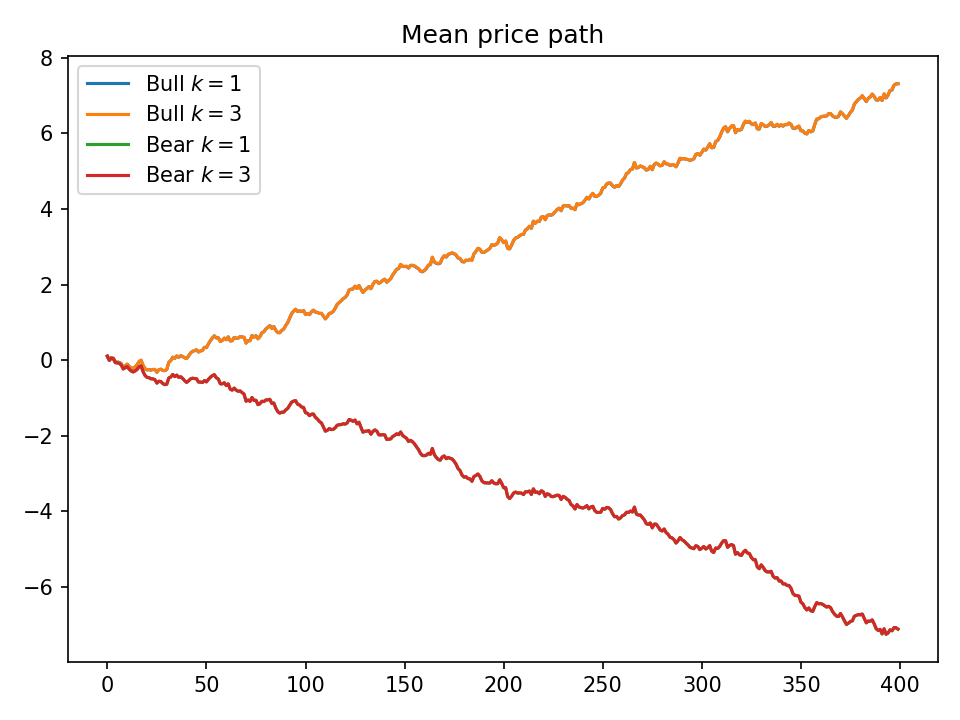
\includegraphics[width=0.48\textwidth]{../paper_artifacts/figures/fig_price_path.png}
  \caption{Mean price path across baseline scenarios (bull/bear regimes; $k\in\{1,3\}$).}
  \label{fig:price_path}
\end{figure}

\begin{figure}[t]
  \centering
  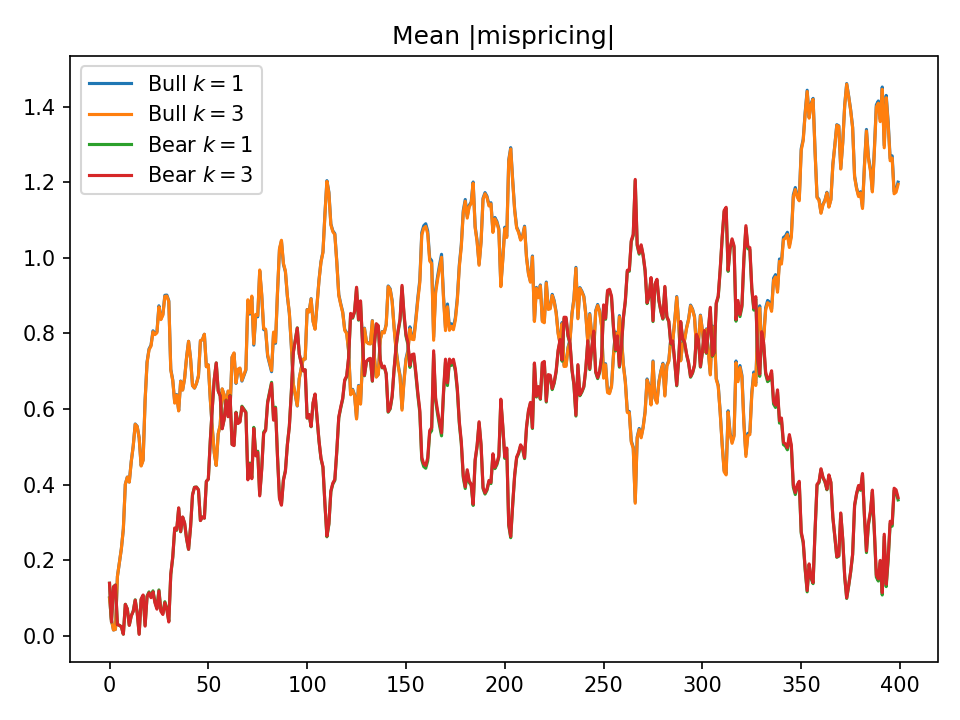
\includegraphics[width=0.48\textwidth]{../paper_artifacts/figures/fig_mispricing.png}
  \caption{Mean absolute mispricing $\E[|p_t-v_t|]$ across baseline scenarios.}
  \label{fig:mispricing}
\end{figure}

\begin{figure}[t]
  \centering
  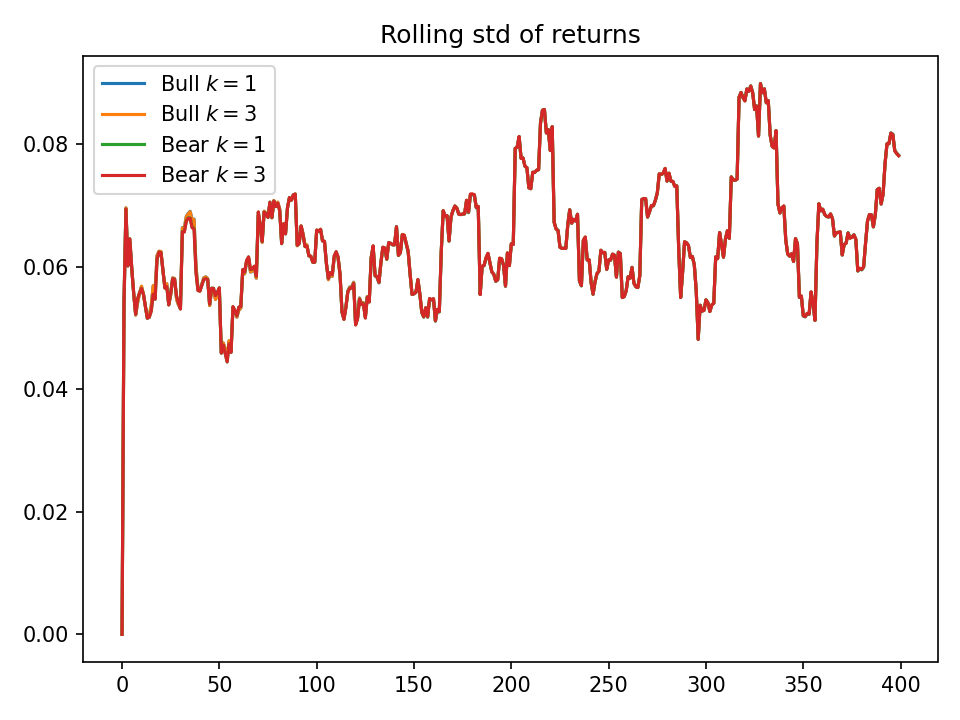
\includegraphics[width=0.48\textwidth]{../paper_artifacts/figures/fig_volatility.png}
  \caption{Rolling volatility proxy (standard deviation of returns) across baseline scenarios.}
  \label{fig:volatility}
\end{figure}

\textbf{Discussion.} The particle simulations are intended as computational evidence for the feedback mechanism highlighted by the model: misperceived signal precision affects belief dispersion and demand, which in turn impacts prices through \eqref{eq:anchored_impact}. A full numerical fixed-point verification for the common-noise mean-field limit (e.g., via conditional-law SPDE solvers) is left for future work.
As a robustness check for the informational simplification (filtering on $\xi_i$ only), the artifact script also produces a ``price-augmented'' filtering variant aligned with the Euler price update: it uses the realized increment $p_{t+1}-p_t$ to form an implicit noisy observation of $v_t$ (Appendix~A). The qualitative $k$-effects on perceived uncertainty and disagreement remain similar in that check (Table~\ref{tab:price_filter}).


\section{Conclusion}
\label{sec:conclusion}
% Section 7: Conclusion

This paper formulates a mean-field game framework for modeling financial markets with heterogeneous overconfident investors. The model couples Bayesian belief updating (with misperceived signal precision) to endogenous price formation through a stochastic anchored-impact price equation. Our main pipeline is a myopic mean-field consistent equilibrium: we derive a checkable \CARA best response under Gaussian price increments and obtain a per-step stock--flow closure linking mean inventory/trading rates to mean belief. Separately, we record continuous-time \CARA/\LQG\ benchmarks as constructive comparisons.

The simulations demonstrate a clean \emph{mechanism separation}: (i) \emph{mispricing levels} are governed primarily by the microstructure regime $(\kappa,\lambda,\phi)$---weak anchoring and high noise trading generate large mispricing and volatility levels; and (ii) \emph{overconfidence ($k$)} robustly loads onto disagreement and trading intensity, but does not materially move price-level mispricing across a broad joint grid (Subsection~\ref{subsec:joint_grid}), even when mispricing levels become large. This structural separation---$k$ shifts belief dispersion and intensity, whereas $(\kappa,\lambda,\phi)$ govern mispricing magnitudes---is the main empirical takeaway. The identification argument (Section~\ref{sec:param_identification}) makes the model empirically testable, clarifying which observable moments pin down the structural parameters.

Several limitations and open questions remain. First, our baseline equilibrium concept and main simulation grid use the myopic \CARA best response under conditionally Gaussian price increments. As a validation check, Subsection~6.4.1 implements an unconstrained finite-horizon \CARA/\LQG\ intertemporal policy and finds similar qualitative $k$-effects. A fully constrained intertemporal formulation and a complete optimal-control MFG verification with endogenous filtering on prices remain future work. Second, while Subsection~\ref{sec:param_identification} provides an identification argument showing which moments pin down $(\kappa,\lambda,\sigma_v,\sigma_\epsilon,\phi)$ in principle, a full empirical calibration targeting these moments from price and volume data would strengthen the quantitative predictions. Third, the single-population framework abstracts from strategic and institutional heterogeneity; multi-population extensions (e.g., retail vs.\ institutional) could produce richer belief distributions and feedback. Finally, Section~III establishes well-posedness of the discrete-time particle system under the per-step contraction/uniqueness condition $0\le B_t<\Delta t$ (Theorems~\ref{thm:contraction} and~\ref{thm:well_posed}). A complete verification of existence/uniqueness conditions for the full intertemporal optimal-control MFG equilibrium (with endogenous filtering on prices) would strengthen the theoretical foundation.


% Statements and Declarations (JEIC). Blind-safe: no institutions/funding in blind mode.

\section*{Statements and Declarations}

\subsection*{Competing interests}
\ifjeicblind
The author(s) declare that they have no known competing financial or non-financial interests.
\else
The authors declare that they have no competing financial or non-financial interests.
\fi

\subsection*{Funding}
\ifjeicblind
The author(s) declare that no specific funding was received for this work.
\else
This work was not supported by external funding.
\fi

\subsection*{Data and code availability}
\ifjeicblind
The author(s) declare that replication materials will be made available upon acceptance.
\else
Code and data used in this study are available from the corresponding author upon reasonable request. Replication package will be provided upon acceptance.
\fi

\subsection*{Author contributions}
\ifjeicblind
The author(s) declare that all contributions are as described in the manuscript.
\else
All authors contributed to the study conception, model development, and writing. Numerical work and drafting were led by the first author.
\fi

\subsection*{Ethics approval}
\ifjeicblind
The author(s) declare that ethics approval is not applicable to this study.
\else
Ethics approval is not applicable (N/A) to this study.
\fi


\appendix
% Appendix: Additional Derivations

\section{Kalman--Bucy Filter With Misperceived Signal Precision}

This appendix summarizes the Kalman--Bucy filter used for belief updating in Section~II.

\subsection{State and Observation Equations}

The (unobserved) fundamental evolves as a linear diffusion
\begin{equation}
dv_t = \mu_v\,dt + \sigma_v\,dW_t,
\end{equation}
and investor $i$ observes a private signal
\begin{equation}
d\xi_{i,t} = v_t\,dt + \sigma_c\,dU_t + \sigma_\epsilon\,dB_{i,t},
\end{equation}
where $W$, $U$, and $B_i$ are independent Brownian motions and $U$ is common across investors.

\subsection{Filter and Riccati Equation}

Let $\hat v_{i,t}$ and $\Sigma_{i,t}$ denote investor $i$'s Kalman--Bucy belief mean and posterior variance computed under the \emph{perceived} measurement-noise variance $R'_i(k_i)$ below.
When $k_i=1$, $\hat v_{i,t}$ coincides with the true conditional mean $\E[v_t\mid \mathcal F^i_t]$ and $\Sigma_{i,t}$ with the true conditional variance.
When $k_i\ne 1$ they are best interpreted as \emph{subjective} filter states under the investor's misspecified noise model.

\subsubsection{Belief-mean SDE and diffusion decomposition}
The belief state is $(\hat v_{i,t},\Sigma_{i,t})$. Only $\hat v_{i,t}$ is stochastic; $\Sigma_{i,t}$ follows a scalar Riccati ODE.
Starting from the Kalman--Bucy form
\begin{equation}\label{eq:kalman_continuous}
\begin{split}
d\hat v_{i,t}&=\mu_v\,dt+K_{i,t}\bigl(d\xi_{i,t}-\hat v_{i,t}\,dt\bigr),\\
K_{i,t}&=\frac{\Sigma_{i,t}}{R'_i},\quad R'_i=\sigma_c^2+\frac{\sigma_\epsilon^2}{k_i}.
\end{split}
\end{equation}
and using the signal SDE $d\xi_{i,t}=v_t\,dt+\sigma_c\,dU_t+\sigma_\epsilon\,dB_{i,t}$, we obtain the explicit diffusion decomposition
\begin{equation}\label{eq:vhat_diffusion_decomp}
d\hat v_{i,t}
=\bigl(\mu_v+K_{i,t}(v_t-\hat v_{i,t})\bigr)\,dt
+K_{i,t}\sigma_c\,dU_t
+K_{i,t}\sigma_\epsilon\,dB_{i,t}.
\end{equation}
Thus the belief-mean diffusion has (i) a \emph{common} component $K_{i,t}\sigma_c\,dU_t$ and (ii) an \emph{idiosyncratic} component $K_{i,t}\sigma_\epsilon\,dB_{i,t}$.
The perceived posterior variance satisfies the Riccati ODE
\begin{equation}\label{eq:riccati}
\dot\Sigma_{i,t}=\sigma_v^2-\frac{\Sigma_{i,t}^2}{R'_i},
\end{equation}
and carries no diffusion term.

Here $R'_i$ is the \emph{perceived} measurement-noise variance. Overconfidence corresponds to $k_i>1$, i.e., investors treat their signal as more precise than it truly is. The common component $\sigma_c\,dU_t$ prevents the law-of-large-numbers collapse of aggregate signal noise in the continuum limit and is the source of common-noise randomness in Section~III.

The scalar Riccati equation admits an explicit solution and converges exponentially to its steady state:
\begin{lemma}[Riccati convergence to steady state]
\label{lem:riccati_convergence}
Fix $R'_i>0$ and $\sigma_v>0$ and let $\Sigma_t$ solve \eqref{eq:riccati} with $\Sigma_0\ge 0$. Then $\Sigma_t\to \Sigma^*:=\sigma_v\sqrt{R'_i}$ as $t\to\infty$ and there exist constants $C,c>0$ (depending on $\Sigma_0,\sigma_v,R'_i$) such that
\begin{equation}
|\Sigma_t-\Sigma^*|\le C e^{-ct},\qquad c=\frac{2\sigma_v}{\sqrt{R'_i}}.
\end{equation}
Consequently, the gain $K_t=\Sigma_t/R'_i$ converges exponentially to $K^*=\sigma_v/\sqrt{R'_i}$.
\end{lemma}

\begin{proof}
Fix $R'_i>0$ and $\sigma_v>0$ and consider the scalar Riccati ODE \eqref{eq:riccati}:
\[
\frac{d\Sigma_t}{dt}=\sigma_v^2-\frac{\Sigma_t^2}{R'_i}.
\]
Let $\Sigma^*:=\sigma_v\sqrt{R'_i}$ (the positive equilibrium) and write $a:=\sigma_v/\sqrt{R'_i}$.
Set $u_t:=\Sigma_t/\Sigma^*$. Then $u_t$ solves
\[
\dot u_t = a(1-u_t^2),\qquad u_0=\Sigma_0/\Sigma^*.
\]
Define the ratio $\rho_t := \frac{1-u_t}{1+u_t}$ (well-defined since $u_t\ge 0$). Differentiating gives
\[
\dot\rho_t = -2a\,\rho_t,
\]
hence $\rho_t=\rho\,e^{-2at}$ with $\rho:=\rho_0=\frac{1-u_0}{1+u_0}=\frac{\Sigma^*-\Sigma_0}{\Sigma^*+\Sigma_0}$.
Solving for $u_t$ yields the explicit solution
\[
\Sigma_t=\Sigma^*\,\frac{1-\rho\,e^{-2at}}{1+\rho\,e^{-2at}}.
\]
In all cases with $\Sigma_0\ge 0$, the denominator satisfies $1+\rho e^{-2at}>0$ and $\Sigma_t\ge 0$ for all $t$, and
$\Sigma_t\to \Sigma^*$ as $t\to\infty$ since $e^{-2at}\to 0$.

Moreover,
\[
\Sigma_t-\Sigma^*=\Sigma^*\Big(\frac{1-\rho e^{-2at}}{1+\rho e^{-2at}}-1\Big)
= -\frac{2\Sigma^*\,\rho\,e^{-2at}}{1+\rho e^{-2at}},
\]
so the convergence is exponential with rate constant $c=2a=2\sigma_v/\sqrt{R'_i}$. For the prefactor, note:
if $\rho\ge 0$ (equivalently $\Sigma_0\le \Sigma^*$), then $1+\rho e^{-2at}\ge 1$ and
\[
|\Sigma_t-\Sigma^*|\le 2\Sigma^*|\rho|\,e^{-2at}.
\]
If $\rho<0$ (equivalently $\Sigma_0>\Sigma^*$), then $1+\rho e^{-2at}\ge 1+\rho = 1-|\rho|$ and
\[
|\Sigma_t-\Sigma^*|\le \frac{2\Sigma^*|\rho|}{1-|\rho|}\,e^{-2at}.
\]
Thus the claimed bound holds with, e.g., $C:=2\Sigma^*|\rho|$ when $\Sigma_0\le \Sigma^*$ and
$C:=\frac{2\Sigma^*|\rho|}{1-|\rho|}$ when $\Sigma_0>\Sigma^*$ (both depending only on $\Sigma_0,\sigma_v,R'_i$).
Since $K_t=\Sigma_t/R'_i$, it follows that
$K_t\to K^*=\Sigma^*/R'_i=\sigma_v/\sqrt{R'_i}$ at the same exponential rate.
\end{proof}

\subsection{Steady State}

In steady state, \eqref{eq:riccati} gives
\begin{equation}
\Sigma_i^* = \sigma_v\sqrt{R'_i} = \sigma_v\sqrt{\sigma_c^2+\frac{\sigma_\epsilon^2}{k_i}},
\end{equation}
and the corresponding steady-state gain is $K_i^* = \Sigma_i^*/R'_i = \sigma_v/\sqrt{R'_i}$.
Thus larger $k$ increases the Kalman gain and reduces perceived posterior variance, generating more aggressive belief updating and, through the trading rule, larger demand responses to perceived mispricing.

\subsection{Discrete-Time Recursion Used in Simulations}

Section~VI implements a discrete-time Kalman recursion consistent with the continuous-time signal model \eqref{eq:kalman_continuous}--\eqref{eq:vhat_diffusion_decomp}. On a grid with step size $\Delta t>0$, the simulated fundamental evolves as
\[
v_{t+1}=v_t+\mu_v\Delta t+\sigma_v\sqrt{\Delta t}\,\varepsilon_{t+1},\qquad \varepsilon_{t+1}\sim\mathcal N(0,1),
\]
 and investor $i$ observes a discrete-time signal obtained from the \emph{flow} observation $d\xi_{i,t}$ by taking increments and normalizing by $\Delta t$:
 \[
 z_{i,t}:=\frac{\xi_{i,t+\Delta t}-\xi_{i,t}}{\Delta t}
 =v_t+\frac{\sigma_c}{\sqrt{\Delta t}}\,\varepsilon^c_t+\frac{\sigma_\epsilon}{\sqrt{\Delta t}}\,\varepsilon^i_{i,t},
 \qquad \varepsilon^c_t,\varepsilon^i_{i,t}\sim\mathcal N(0,1),
 \]
 where $\varepsilon^c_t$ is common across investors and $\varepsilon^i_{i,t}$ is idiosyncratic. (With $\Delta t=1$, this reduces to $z_{i,t}=v_t+\sigma_c\varepsilon^c_t+\sigma_\epsilon\varepsilon^i_{i,t}$, matching the implementation.)
Thus $\Var(z_{i,t}\mid v_t)=(\sigma_c^2+\sigma_\epsilon^2)/\Delta t$; write $R(\Delta t):=(\sigma_c^2+\sigma_\epsilon^2)/\Delta t$ for the objective measurement variance.
Overconfidence scales only the idiosyncratic component, so the perceived measurement variance for $z_{i,t}$ is
 \[
 R'_i(\Delta t)=\frac{\sigma_c^2+\sigma_\epsilon^2/k_i}{\Delta t}.
 \]
 Let $(\hat v_{i,t},\Sigma_{i,t})$ denote the posterior mean/variance after processing $z_{i,t}$. The discrete-time Kalman recursion is:
  \begin{align*}
   \Sigma^-_{i,t} &= \Sigma_{i,t-1}+\sigma_v^2\Delta t,\\
  K_{i,t} &= \frac{\Sigma^-_{i,t}}{\Sigma^-_{i,t}+R'_i(\Delta t)},\\
   \hat v_{i,t} &= \hat v_{i,t-1}+\mu_v\Delta t+K_{i,t}\bigl(z_{i,t}-(\hat v_{i,t-1}+\mu_v\Delta t)\bigr),\\
   \Sigma_{i,t} &= (1-K_{i,t})\Sigma^-_{i,t}.
  \end{align*}
 
 Given the mean trading rate $\bar u_t$ (with $\bar u_t\Delta t=\Delta\bar x_t$ under the stock--flow timing), the discrete-time price update (Euler form of \eqref{eq:anchored_impact}) used in the code is
 \[
\begin{aligned}
 p_{t+1}
 &= p_t+\kappa(v_t-p_t)\Delta t+\lambda \bar u_t\Delta t + \phi \sqrt{\Delta t}\,\varepsilon^\eta_{t+1},\\
 \varepsilon^\eta_{t+1}&\sim\mathcal N(0,1).
\end{aligned}
 \]

\subsection{Price-Augmented Filtering (Robustness Variant)}
 
 Because prices are public and informative under \eqref{eq:anchored_impact}, a fully consistent informational equilibrium would incorporate $p$ into the observation set and solve a joint filtering/fixed-point problem. As a robustness check aligned with the implemented Euler update above, we construct an \emph{implicit} noisy observation of $v_t$ from the realized price increment:
 \[
 \tilde v^{(p)}_t
 := p_t+\frac{(p_{t+1}-p_t)-\lambda \bar u_t\Delta t}{\kappa\Delta t}
  = v_t+\frac{\phi}{\kappa\sqrt{\Delta t}}\,\varepsilon^\eta_{t+1}.
  \]
 Conditional on $\mathcal F_t$, this yields a Gaussian observation of $v_t$ with measurement variance
 $R_p=\phi^2/(\kappa^2\Delta t)$ (scaled by a factor $\sigma_{p,\mathrm{obs}}^2$ in the code to probe robustness). We then apply an additional Kalman update using $\tilde v^{(p)}_t$ as a measurement (after processing the private signal), holding the state prediction fixed. Table~\ref{tab:price_filter} summarizes the impact of this price-consistent augmentation on the reported $k$-effects.


\bibliographystyle{plainnat}
\bibliography{refs}

\end{document}
